\begin{chapter}{GZ-CMD: política de decisão e revisão assistida}\label{cap:estudo4}

O quarto objetivo específico é desenvolver e avaliar o GZ-CMD, política de decisão por \textit{expected loss} com custos assimétricos, calibração fora da amostra e revisão assistida por modelo de linguagem de grande porte. Aplica-se aos potenciais pares não aceitos pelo corte do OpenRecLink. Comparam-se vínculos recuperados, falsos positivos, encaminhamentos ao revisor humano, custo e carga de revisão com a referência operacional, com estratégias de corte único e de duas fronteiras e com as ordenações O1 a O4 abaixo do corte.\footnote{O1 ordena pelo escore do OpenRecLink; O2, pela nota do Comparador de Registros; O3, pela probabilidade calibrada do classificador na base inteira; O4, pela probabilidade recalibrada abaixo do corte.}

A tuberculose é a condição marcadora adotada para investigar a qualificação dos dados vinculados entre SIM e Sinan-TB (Seções~\ref{sec:tb-marcadora} e~\ref{sec:e3-discussao-impacto}). Os resultados deste capítulo avaliam a política e suas comparações na coorte estudada, não sustentam por si uma proposta de adoção ou ganho epidemiológico fora dela \cite{Jardim2026phdrepo}.

Persistem lacunas após os resultados dos Capítulos~\ref{cap:estudo2} e~\ref{cap:estudo3}. Custos assimétricos representam preferências sobre as consequências dos erros, não valores econômicos medidos: perder um vínculo pode manter sem correção o encerramento da notificação existente e gerar nova notificação do mesmo caso, enquanto um falso vínculo pode produzir investigação indevida ou encerramento incorreto de caso de pessoa viva. Na confirmação, a política atribui ao FP custo cinco vezes maior que ao FN. Essa preferência foi fixada pelo autor, não estimada com profissionais do serviço. A baixa portabilidade de limiares sob variação de prevalência e completude \cite{Shaw2022biases} soma-se ao trabalho de revisão dos potenciais pares não decididos \cite{Christen2012book,Coeli2021suboptimal}.

O GZ-CMD é uma política de decisão por \textit{expected loss} no \textit{linkage} probabilístico, também denominado relacionamento de registros (\textit{record linkage}). O nome \textit{Grey-Zone: Calibrated Mixture-of-experts + Conformal Deferral + Constrained Matching}, nome histórico cuja correspondência com os componentes implementados é discutida no Glossário, remete à região entre limiares de Fellegi e Sunter, a região não decidida pela regra automática (Seção~\ref{sec:area-cinza}). Nos resultados, área cinza da nota designa $[5,9)$ do CdR; região abaixo do corte designa onde o arranjo sequencial decide, preservando as aceitações do corte e aplicando a política abaixo dele. Sua aplicação depois do corte do OpenRecLink trata a revisão abaixo dele como problema de decisão. A referência operacional é esse corte, isolado ou seguido da revisão clerical de origem; os cortes da nota do Comparador de Registros (CdR) constituem cenários hipotéticos (Tabela~\ref{tab:cap8-referencia}). Integram-se classificação, calibração supervisionada fora da amostra, guardas (regras fixas) e revisão assistida por modelos de linguagem, com calibração por conjuntos âncora (pares de nota extrema usados para calibrar) avaliada como alternativa.

Na versão v3.1, o classificador é incorporado a uma política com quatro componentes: guardas nos extremos da nota do CdR; calibração isotônica fora da amostra, agrupada por REFREC; decisão por \textit{expected loss} entre vínculo, não vínculo, LLM e revisor humano; e revisão assistida a partir dos subescores efetivamente enviados, com inconclusivos ao humano. O ajuste sigmoide por momentos nas âncoras é alternativa distinta do \textit{Platt scaling} supervisionado da nota e de P-Platt, que calibra o logit da probabilidade bruta abaixo do corte e é tratado como sensibilidade (Seção~\ref{sec:e4-arranjo-metodo}). A regra histórica de homonímia combina nota, discordância de nascimento e ausência de evidência de endereço; não exige divergência de nome ou nome da mãe e não pertence à v3.1 (Seção~\ref{sec:e4-regras-guarda}). O GZ-CMD é biblioteca sem interface gráfica; a captura do CdR no Estudo~1 não representa uma interface da política.\footnote{v3.1 identifica a política de quatro ações, com revisão humana distinta da revisão LLM.}

\section{Método}\label{sec:e4-metodo}

O resultado principal é o arranjo sequencial com registro interno anterior à avaliação com os \textit{labels} (S3), avaliação precedida pela simulação sem API (S1) e pelas chamadas ao LLM (S2); trata-se de registro versionado no repositório, não registro público (Seções~\ref{sec:e4-arranjo-metodo} e~\ref{sec:e4-arranjo}). O corte aceita os 211 potenciais pares no corte ou acima dele, todos com PAR~=~1. A política v3.1, recalibrada abaixo do corte, decide os demais, que incluem os 36 vínculos com PAR~=~2. A referência de carga é o cenário condicional da Seção~\ref{sec:padrao-ouro}, não o teto de candidatos. A cascata sobre a base inteira fixou o revisor de referência (modelo de linguagem adotado para estimar as proporções de erro) e as proporções de erro usadas no desenvolvimento, permanecendo como comparação (Seção~\ref{sec:e4-cascata}) \cite{Jardim2026phdrepo}.\footnote{v3.1 identifica a política de quatro ações, com revisão humana distinta da revisão LLM.}

O GZ-CMD organiza a tomada de decisão a partir da probabilidade de vínculo, das regras de guarda, do \textit{expected loss engine} e da revisão assistida. Distinguem-se a versão v3, utilizada nos experimentos históricos, e a política v3.1 (Seção~\ref{sec:e4-politica-v31}), que emprega classificação supervisionada com calibração isotônica fora da amostra, agrupada por REFREC, e compara explicitamente decisões automáticas, revisão por modelo de linguagem de grande porte (LLM) e revisão humana.\footnote{v3 identifica a política histórica de três ações ou, nas instruções do LLM, a versão que solicita as saídas do motor.}

Na versão histórica v3, os limiares convencionais de nota 5 e 9 não constituíam duas guardas rígidas: o limiar da guarda de aceitação era 10,0, com exigências adicionais de consistência, e apenas quatro pares foram aceitos por essa guarda; a guarda inferior de nota era $<3$, não $<5$. O lote selecionado pelo motor incluiu 22 pares com nota final do CdR $\geq9$, sendo um com nota $\geq10$ e 21 em $[9,10)$. Na área cinza da nota, definida por $5\leq\text{nota}<9$, 2.821 pares foram rejeitados pela guarda temporal no artefato histórico. Esse descarte não pode ser atribuído integralmente a $EVR\leq0$, pois 202 desses pares tinham $EVR>0$. Esses resultados distinguem as decisões históricas dos critérios pretendidos; a política v3.1 corrige os cortes de nota e explicita a separação entre guardas e decisões automáticas por custo esperado.\footnote{EVR é o valor esperado da revisão.}

Os registros, o recorte temporal, a blocagem e a referência operacional são os descritos no Capítulo~\ref{cap:dados}, com 61.696 potenciais pares (247 vínculos, 61.449 não-pares); as limitações da referência operacional (Seções~\ref{sec:padrao-ouro} e~\ref{sec:concl-limitacoes}) são particularmente relevantes no GZ-CMD nas regiões de maior ambiguidade do escore, onde erros residuais de rotulagem podem persistir.

\subsection{Delineamento experimental}\label{sec:e4-delineamento}

O arranjo sequencial é o resultado principal, com registro interno \texttt{8c16a41}; sua análise de estabilidade tem registro próprio, \texttt{3ade1c7}, e não é confirmatória (Seção~\ref{sec:e4-arranjo-metodo}). As comparações de mesma carga, esforço, uso do LLM como filtro, subamostragem e cenários humanos são análises exploratórias \textit{post hoc}, descritas na Seção~\ref{sec:e4-exploratorias-metodo}.

Na ablação do GZ-CMD, foram realizadas cinco rodadas de particionamento em treinamento e teste na partição agrupada por COMPREC (registro do Sinan), distinta do agrupamento por REFREC adotado na v3.1, com fração de teste de 30\% e sementes de 42 a 46, conforme as tabelas da Seção~\ref{sec:apendice-ablacao}. Esse protocolo difere da validação cruzada em cinco partições e do QW1 $5 \times 5$ descritos na Seção~\ref{sec:analises-complementares}. As métricas são reportadas como média e desvio-padrão entre rodadas, com comparações exploratórias por teste t pareado ($\alpha=0{,}05$). As cinco partições de teste se sobrepõem; o teste t pareado supõe rodadas independentes e tende a produzir valores de $p$ otimistas. No experimento de revisão assistida, foram avaliados os 1.410 pares selecionados pelo motor v3 entre os 61.696 potenciais pares do extrato, com \textit{Platt scaling} ajustado nos próprios \textit{labels}; esse universo não representa revisão humana integral observada.\footnote{QW1 é a comparação complementar de classificadores tabulares.}

\subsection{Representação dos pares e engenharia de atributos}\label{sec:e4-representacao}

A representação dos potenciais pares baseia-se no vetor de 29 subescores do Comparador de Registros \cite{Jardim2025comparador,Lucena2013algoritmos}, cuja descrição técnica já foi apresentada na Seção \ref{sec:comparador-registros}. Neste capítulo, o foco recai sobre o efeito operacional da representação, sobretudo na área cinza da nota do CdR, definida por $[5,9)$, sem repetir a fundamentação apresentada no Capítulo~\ref{cap:estudo1}.\footnote{CdR designa o Comparador de Registros.}

As Medidas Contínuas de Diferença de Datas (MACD), denominação histórica, reúnem atributos derivados das datas de nascimento: diferença absoluta em dias convertida em anos e limitada a 20 anos; indicadores de coincidência de ano, mês e dia e sua proporção; proximidade de até 30 e até sete dias; e interações do nome idêntico com diferença de pelo menos cinco anos e com a diferença limitada a 20 anos (\path{gzcmd/loader.py}). Nome idêntico exige concordância dos fragmentos e proporção de fragmentos iguais de pelo menos 0,95. Não incluem diferença entre óbito e notificação e não são todas contínuas. O efeito da inclusão desse conjunto de atributos é analisado na Seção~\ref{sec:e4-exp1}, com os valores de ablação das tabelas da Seção~\ref{sec:apendice-ablacao}.

\subsection{Calibração por âncoras e faixas de confiança}
\label{sec:e4-calibracao}

Em contraste com o esquema clássico de Fellegi e Sunter \cite{Fellegi1969theory}, a proposta inicial adotou calibração discriminativa dos escores brutos. A função sigmoide
\[
p_{cal}(s)=\frac{1}{1+\exp\left(-\left(\alpha s+\beta\right)\right)}
\]
foi utilizada como estimativa de $P(y{=}1\mid s)$, a probabilidade de que o potencial par seja um vínculo verdadeiro dado o escore observado. A forma sigmoide é uma hipótese de modelagem. Seus parâmetros são ajustados a partir de conjuntos âncora, isto é, subconjuntos de pares com status presumido de alta confiança a partir de critérios empíricos de escore extremo: os conjuntos positivos ($A^+$, pares com escore elevado) e negativos ($A^-$, pares com escore muito baixo). O ajuste dispensa novos \textit{labels} em tempo de operação e preserva a ordenação dos escores. Sua interpretação probabilística exige validação com \textit{labels}, tendo a isotônica supervisionada como referência neste estudo; a dispensa de novos \textit{labels} na operação não demonstra calibração absoluta sem supervisão.

Os parâmetros $\alpha$ e $\beta$ são obtidos por restrições de média alvo sobre as âncoras,
\[
\mathbb{E}_{s\in A^+}[\sigma(\alpha s+\beta)] = r^+,
\qquad
\mathbb{E}_{s\in A^-}[\sigma(\alpha s+\beta)] = r^-.
\]
Os alvos satisfazem $0<r^-<r^+<1$, pois os valores 0 e 1 não são atingidos por uma sigmoide com parâmetros finitos. Essas restrições controlam apenas as duas médias nas âncoras, não garantindo calibração local na região intermediária ou estabilidade sob deriva. As limitações de identificabilidade, estabilidade numérica e contaminação são discutidas na Seção~\ref{sec:apendice-formalizacao}, em especial na Proposição \ref{prop:anchor-contamination-bias}, e requerem validação com dados rotulados independentes.

Na versão v3, a estimativa de probabilidade de vínculo $p_{cal}$ produzida pela sigmoide delimitava três regiões decisórias por dois limiares: $t_{high}$ (limiar superior de confiança) e $t_{low}$ (limiar inferior de confiança). Pares com $p_{cal}\geq t_{high}$ eram classificados como alta confiança de vínculo; pares com $p_{cal}\leq t_{low}$, como não-vínculo; e pares na faixa intermediária ($t_{low}<p_{cal}<t_{high}$) eram avaliados pelo \textit{expected loss engine}. Essas regiões de probabilidade não redefinem a área cinza da nota, que neste capítulo corresponde a notas finais do comparador em $[5,9)$, nem se confundem com as seis faixas operacionais dessa nota, utilizadas para calibração, perfil de erro do revisor e monitoramento.

\subsection{Classificador supervisionado e calibração fora da amostra}
\label{sec:e4-classificador-oof}

A transformação da nota final por \textit{Platt scaling} não acrescenta informação discriminativa ao comparador: por ser estritamente crescente, mantém a ordenação da nota, com correlação de Spearman praticamente 1 entre ambas as colunas de \texttt{data/pcal\_ml\_oof.csv}. Para utilizar conjuntamente as comparações de campos, ajustou-se um XGBoost com 300 árvores sobre 30 atributos do extrato, correspondentes aos 29 subescores e à nota final, sem identificadores, datas brutas ou a referência operacional entre os preditores; as MACD não integram esses 30 atributos, embora possam compor o dossiê do LLM. A probabilidade resultante, denominada \texttt{p\_cal\_ml}, foi produzida por validação cruzada aninhada, com cinco partições externas, cinco internas, semente 42 e agrupamento por registro de referência (REFREC) nos dois níveis, conforme a implementação e os metadados desse artefato e \texttt{gzcmd/M\_oof\_grupos\_pr7.md}. A família e os hiperparâmetros do XGBoost provêm do QW1, avaliado nesta mesma base; as métricas OOF não incorporam essa seleção \cite{Jardim2026phdrepo}.\footnote{MACD designa as Medidas Contínuas de Diferença de Datas, atributos derivados do nascimento; QW1 é a comparação complementar de classificadores tabulares.}

Em cada partição externa, as probabilidades fora da amostra (\textit{out-of-fold}, OOF) das cinco partições internas do treinamento alimentaram o ajuste isotônico. O classificador reajustado no treinamento externo produziu os escores do teste externo, aos quais se aplicou esse calibrador, sem acesso aos \textit{labels} do teste em qualquer dos dois ajustes. O particionamento agrupou os potenciais pares pelo registro de referência (REFREC, que identifica o registro do SIM), de modo que um mesmo registro não contribui para treino e teste da mesma partição; o lado comparado (COMPREC, que identifica o registro do Sinan-TB) não é agrupado simultaneamente, e o agrupamento por COMPREC foi examinado como análise de sensibilidade. Essa avaliação não equivale a validação externa.

Nos 21.620 potenciais pares da área cinza da nota, com 151 vínculos, a probabilidade isotônica OOF agrupada por REFREC apresentou área sob a curva ROC (AUC) de 0,995 e precisão média (AP) de 0,862; a mediana da probabilidade nos vínculos foi de 0,895, contra 0,026 com \textit{Platt scaling} da nota. O agrupamento reduziu o AP e a mediana nos vínculos em relação à partição por potencial par (AUC de 0,993, AP de 0,907 e mediana de 0,982), e o agrupamento por COMPREC, examinado como sensibilidade, produziu 0,994, 0,911 e 0,981. O comparador histórico apresentou AUC de 0,873 e AP de 0,216 nesse recorte, mas seu ajuste utilizou os próprios \textit{labels} avaliados e não constitui referência de calibração OOF. Os valores constam de \texttt{data/pcal\_ml\_oof\_grupos\_metricas.csv} e, para a nota, de \texttt{data/ancoras\_beta\_validacao.csv} \cite{Jardim2026phdrepo}.

A Tabela~\ref{tab:e4-desempenho-faixas-oof} desagrega esse estimador por faixa da nota final. O estimador usa apenas os 30 atributos descritos acima (29 subescores e a nota final), sem variáveis de óbito. Na área cinza da nota, com limiar 0,5, recupera 119 dos 151 vínculos (sensibilidade de 0,788) com 28 falsos positivos (precisão de 0,810); a precisão é de 0,632 na faixa de 5 a 6 e de 0,644 na faixa de 8 a 9, e abaixo de 5 nenhum dos três vínculos atinge 0,5. Cada faixa reúne poucas dezenas de vínculos (17 a 57 nas faixas da área cinza da nota), e a faixa de 8 a 9 tem 34 vínculos em 102 pares; a tabela apresenta intervalos de Wilson de 95\% para sensibilidade e precisão, descritivos e sem ajuste para dependência entre pares, e omite AUC e AP quando a classe minoritária tem menos de cinco casos. O limiar 0,5 é ilustrativo e foi fixado antes da análise: a política v3.1 decide por \textit{expected loss}, não por limiar fixo, de modo que a tabela caracteriza a discriminação do estimador por faixa, não o desempenho da política. Os valores constam de \texttt{data/desempenho\_faixas\_oof\_refrec.csv}, gerado por \texttt{scripts/desempenho\_faixas\_oof\_refrec.py} \cite{Jardim2026phdrepo}.

% Gerado por scripts/gerar_tabelas_nb03_faixas.py de data/desempenho_faixas_oof_refrec.csv
\begin{table}[!htbp]
\centering
\scriptsize
\setlength{\tabcolsep}{3pt}
\caption{Desempenho do estimador \texttt{p\_cal\_ml} (XGBoost com calibração isotônica) por faixa da nota final $v$ do Comparador de Registros (CdR), nos 61.696 potenciais pares e 247 pares verdadeiros do extrato. As probabilidades são estimativas fora da amostra agrupadas por REFREC; contagens e razões usam o limiar 0,5, fixado antes da análise e não otimizado. AUC e AP: área sob a curva ROC e precisão média; Brier: escore de Brier. n.d.: AUC e AP não exibidas quando a classe minoritária tem menos de cinco casos, ou razão não definida por denominador zero.}
\label{tab:e4-desempenho-faixas-oof}
\begin{tabular}{@{}lrrcccccccc@{}}
\toprule
Faixa & Pares & \shortstack{Pares\\verdadeiros} & AUC & AP & Brier & VP & FP & FN & Sensib. & VPP \\
\midrule
$<5$ & 39.981 & 3 & n.d. & n.d. & 0,0001 & 0 & 2 & 3 & \shortstack{0,000\\(0,000; 0,561)} & \shortstack{0,000\\(0,000; 0,658)} \\
5-6 & 14.263 & 17 & 1,000 & 0,721 & 0,0007 & 12 & 7 & 5 & \shortstack{0,706\\(0,469; 0,867)} & \shortstack{0,632\\(0,410; 0,809)} \\
6-7 & 6.175 & 57 & 0,984 & 0,855 & 0,0023 & 45 & 1 & 12 & \shortstack{0,789\\(0,667; 0,875)} & \shortstack{0,978\\(0,887; 0,996)} \\
7-8 & 1.080 & 43 & 0,995 & 0,922 & 0,0096 & 33 & 4 & 10 & \shortstack{0,767\\(0,623; 0,868)} & \shortstack{0,892\\(0,753; 0,957)} \\
8-9 & 102 & 34 & 0,913 & 0,873 & 0,1360 & 29 & 16 & 5 & \shortstack{0,853\\(0,699; 0,936)} & \shortstack{0,644\\(0,498; 0,768)} \\
$\geq9$ & 95 & 93 & n.d. & n.d. & 0,0373 & 89 & 2 & 4 & \shortstack{0,957\\(0,895; 0,983)} & \shortstack{0,978\\(0,923; 0,994)} \\
\midrule
Faixa intermediária & 21.620 & 151 & 0,995 & 0,862 & 0,0022 & 119 & 28 & 32 & \shortstack{0,788\\(0,716; 0,846)} & \shortstack{0,810\\(0,738; 0,865)} \\
Total & 61.696 & 247 & 0,996 & 0,911 & 0,0009 & 208 & 32 & 39 & \shortstack{0,842\\(0,791; 0,882)} & \shortstack{0,867\\(0,818; 0,904)} \\
\bottomrule
\end{tabular}

\vspace{2pt}
\par\footnotesize Nota: faixas fechadas à esquerda e abertas à direita. VP, FP e FN são verdadeiros positivos, falsos positivos e falsos negativos com \texttt{p\_cal\_ml} $\geq 0{,}5$. Faixa intermediária: $5\leq v<9$. Entre parênteses, IC de Wilson de 95\% para sensibilidade e VPP, descritivos e sem ajuste para dependência entre pares. Fonte: \texttt{data/desempenho\_faixas\_oof\_refrec.csv}.
\par\footnotesize REFREC identifica o registro do SIM. OOF: probabilidades produzidas fora da amostra de treinamento. CdR: Comparador de Registros; $v$: sua nota final.
\end{table}


O ajuste por âncoras sobre a margem OOF do XGBoost preservou sua capacidade de ordenação, mas não forneceu probabilidades absolutas comparáveis às da isotônica supervisionada. Essa distinção, examinada também na extensão Beta por momentos da Seção~\ref{sec:e4-calibracao-beta}, impede interpretar a mediana dos vínculos (0,895) como demonstração de calibração sem gabarito. A política v3.1 utiliza a isotônica supervisionada; as alternativas por âncoras permanecem avaliações de supervisão agregada, com alcance delimitado pelas Seções~\ref{sec:e4-validacao-ancoras} e~\ref{sec:e4-calibracao-beta}.

\subsection{Validação empírica dos conjuntos âncora}
\label{sec:e4-validacao-ancoras}

A Tabela \ref{tab:cap8-ancoras} confronta os conjuntos âncora com a referência operacional no extrato pseudonimizado ($N=61.696$ potenciais pares, 247 vínculos). Os limiares da nota do CdR que definem as âncoras ($\geq9$ e $<5$) não são as guardas executadas pela v3. O conjunto $A^+$ contém 95 pares, com proporção de vínculos de 97,9\%; $A^-$ contém 39.981, dos quais três são vínculos. Os alvos medidos são $r^+=0{,}979$ e $r^-=0{,}00008$, este último igual a $3/39.981$ arredondado a cinco casas no \textit{script}, escolhido após inspeção dos \textit{labels}, não independentemente deles (\path{scripts/validar_ancoras.py}).\footnote{CdR designa o Comparador de Registros.}

% Gerado por scripts/validar_ancoras.py sobre data/COMPARADORSEMIDENT.csv
\begin{table}[!ht]
\centering
\caption{Validação dos conjuntos âncora contra a referência operacional (extrato pseudonimizado, $N = 61.696$ pares, 247 pares verdadeiros).}
\label{tab:cap8-ancoras}
\begin{tabular}{|l|c|r|r|r|c|}
\hline
Conjunto & Critério & $N$ & Acertos & Erros & Pureza (\%) \\
\hline
$A^+$ (âncoras positivas) & $s\geq 9{,}0$ & 95 & 93 & 2 & 97,89 \\
\hline
$A^-$ (âncoras negativas) & $s<5{,}0$ & 39.981 & 39.978 & 3 & 99,99 \\
\hline
\end{tabular}
\par\footnotesize Conjuntos âncora: potenciais pares de nota extrema usados para calibrar. CdR: Comparador de Registros.
\end{table}


A validação da calibração exige comparação com \textit{labels}, e os alvos $r^+$ e $r^-$ dependem de como são fixados. Distinguem-se três cenários: \textit{Platt scaling} supervisionado sobre a nota, com os 247 vínculos; alvos medidos nas âncoras ($r^+=0{,}979$, $r^-=0{,}00008$), com uso dos \textit{labels} para fixar duas constantes; e alvos a priori $r^+=0{,}99$ e $r^-=0{,}001$, sem medir essas prevalências. Estes últimos são os valores da análise de sensibilidade, não o par $0{,}98/0{,}001$ da configuração histórica. A proporção observada nas faixas $[5,6)$, $[6,7)$, $[7,8)$ e $[8,9)$ foi de 0,1\%, 0,9\%, 4,0\% e 33,3\%. A calibração supervisionada estimou 0,1\%, 0,8\%, 5,3\% e 34,3\% (Brier de 0,0062); com prevalências medidas, 0,2\%, 1,7\%, 13,0\% e 63,3\% (Brier de 0,0072); com alvos a priori, 1,5\%, 9,2\%, 37,8\% e 83,6\% (Brier de 0,0165). Com $r^-=0{,}0001$, variante a priori distinta do alvo medido, e $r^+=0{,}99$, o Brier cai para 0,0090. Os valores constam de \path{data/ancoras_calibracao_faixas.csv} e \path{scripts/validar_ancoras.py}. As âncoras superestimam a probabilidade nas faixas $[7,9)$, mais ainda com alvos a priori. A superestimação nas faixas superiores não sustenta substituir a calibração supervisionada. Os pesos extremos do modelo de origem, $-12{,}85$ e $+16{,}11$, são cálculos da tese com os parâmetros $m$ e $u$, em base 2, não valores transcritos da monografia (\path{data/ancoras_beta_ajustes.json}, \texttt{unit\_audit}; Seção~\ref{sec:padrao-ouro}).

O escore de Brier na área cinza da nota é dominado pela baixa prevalência (151 vínculos em 21.620 pares), de modo que um preditor constante obteria cerca de 0,0069. Como toda sigmoide é transformação monótona da nota final, as três calibrações têm discriminação idêntica (área sob a curva ROC de 0,873 na área cinza da nota); a calibração altera a escala de probabilidade utilizada na decisão por custo esperado. Os conjuntos âncora situam-se fora da área cinza da nota ($v\geq 9$ e $v<5$), enquanto a avaliação se dá dentro dela: os \textit{labels} entram na calibração por âncoras apenas como duas prevalências de regiões disjuntas da região avaliada, ao passo que a calibração supervisionada utiliza os \textit{labels} da própria área cinza da nota.

A Tabela~\ref{tab:cap8-ancoras-decisao} avalia, por isso, o efeito da calibração sobre a decisão, executando o próprio motor de decisão do \textit{framework} (política histórica v3 da Seção~\ref{sec:e4-motor-politica}) sobre a área cinza da nota, sem regras de guarda nem restrições de consistência, com os custos, tetos, orçamento e proporções de erro do revisor da configuração histórica; o ajuste por âncoras é o do pacote publicado \cite{Jardim2026gzcmd}. No modo vigilância, a calibração por âncoras com prevalências medidas produziu menos falsos negativos automáticos que a supervisionada (55 contra 69), nenhum falso positivo automático e menor perda realizada (3.250 contra 3.848 com revisor perfeito; 4.505 contra 4.817 com as proporções de erro configuradas), ao custo de maior volume de revisão (2.000, no teto do orçamento, contra 1.590). O viés de superestimação é, nesse modo, conservador: desloca pares para a revisão em vez de descartá-los. No modo confirmação, o mesmo viés amplia a revisão (647 contra 210) e, com revisor imperfeito e custo elevado de falso positivo, eleva a perda (4.276 contra 2.777), de modo que a calibração por âncoras não é recomendada nesse modo sem validação com \textit{labels}. Os alvos a priori confirmam que $r^-$ é o parâmetro crítico: com $r^- = 0{,}001$, a vigilância incorre em 172 falsos positivos automáticos; com $r^- = 0{,}0001$, em 14.

% Gerado por scripts/validar_ancoras.py (simulação simplificada da política de decisão na área cinza)
\begin{table}[!ht]
\centering
\caption{Efeito da calibração sobre a decisão por custo esperado na área cinza da nota do CdR ($5\leq v<9$; 21.620 pares, 151 vínculos), por modo operacional. Executado pelo motor de decisão do \textit{framework}, sem regras de guarda nem restrições de consistência; custos, tetos, orçamento e proporções de erro do revisor conforme a configuração. Perda realizada com revisor perfeito e com as proporções de erro configuradas.}
\label{tab:cap8-ancoras-decisao}
\scriptsize
\setlength{\tabcolsep}{3pt}
\begin{tabular}{|l|l|r|r|r|r|r|}
\hline
Modo & Calibração & Revisão & FN auto & FP auto & Perda (rev.\ perfeito) & Perda (rev.\ config.) \\
\hline
Vigilância & Supervisionada (\textit{Platt scaling}, 247 \textit{labels}) & 1.590 & 69 & 0 & 3.848 & 4.817 \\
Vigilância & Âncoras, prevalências medidas & 2.000 & 55 & 0 & 3.250 & 4.505 \\
Vigilância & Âncoras a priori ($0{,}99$ / $0{,}001$) & 2.000 & 54 & 172 & 4.920 & 6.134 \\
Vigilância & Âncoras a priori ($0{,}99$ / $0{,}0001$) & 2.000 & 55 & 14 & 3.390 & 4.617 \\
\hline
Confirmação & Supervisionada (\textit{Platt scaling}, 247 \textit{labels}) & 210 & 107 & 0 & 2.192 & 2.777 \\
Confirmação & Âncoras, prevalências medidas & 647 & 91 & 0 & 1.982 & 4.276 \\
Confirmação & Âncoras a priori ($0{,}99$ / $0{,}001$) & 1.000 & 77 & 0 & 1.790 & 5.463 \\
Confirmação & Âncoras a priori ($0{,}99$ / $0{,}0001$) & 1.000 & 76 & 0 & 1.770 & 5.440 \\
\hline
\end{tabular}
\par\footnotesize Conjuntos âncora: potenciais pares de nota extrema usados para calibrar. CdR: Comparador de Registros; $v$: sua nota final. A área cinza da nota não é a região abaixo do corte do OpenRecLink.
\end{table}


A calibração por âncoras com prevalências medidas utiliza supervisão restrita às âncoras, incluindo a escolha a posteriori de $r^-=0{,}00008$. Os resultados operacionais na vigilância não demonstram calibração local, e a confirmação requer validação supervisionada. Os valores foram gerados por \path{scripts/validar_ancoras.py} \cite{Jardim2026phdrepo}.

\clearpage
\subsection{Calibração Beta por momentos}
\label{sec:e4-calibracao-beta}

Na margem OOF do XGBoost, com partição agrupada por REFREC nos níveis externo e interno, o ajuste sigmoide por momentos nas âncoras apresentou ECE de $0{,}002537$, contra $0{,}001125$ da isotônica supervisionada aninhada, prevendo $0{,}995$ onde se observou $0{,}847$ em $p\geq0{,}9$. O ajuste global por momentos sobre essas margens não constitui calibração inteiramente aninhada, ao contrário da referência isotônica. A justificativa gaussiana de Platt, com variâncias iguais, pode ser inadequada às margens saturadas de árvores; duas médias extremas tampouco identificam a forma intermediária. Adaptou-se a família Beta de \citeonline{Kull2017beta} ao ajuste por momentos:
\begin{equation}
p_{\mathrm{B}}(s)=\sigma\!\left(a\ln s-b\ln(1-s)+c\right),
\qquad a,b\geq0,
\label{eq:cap8-beta-momentos}
\end{equation}
com $s=\sigma(z)$, sendo $z$ a margem fora da amostra do XGBoost e $s$ truncada em $[10^{-6},1-10^{-6}]$.

As médias alvo foram medidas em $A^- = \{v<5\}$, $A^+_1=\{9\leq v<9{,}5\}$ e $A^+_2=\{v\geq9{,}5\}$, com 3/39.981, 18/18 e 75/77 vínculos, respectivamente; $v$ designa a nota do comparador, distinta do escore do \textit{linkage}. Beta+ acrescentou $\sum_{5\leq v<9}p_{\mathrm{B}}=\widehat{E}_{\mathrm{cinza}}$, soma de posteriores de Fellegi e Sunter obtidos do peso disponível, com prevalência estimada por EM sem \textit{labels}. Minimizaram-se resíduos das médias ponderados pelo inverso da variância binomial estimada, com múltiplas inicializações e semente 42. A Tabela~\ref{tab:cap8-ancoras-beta} avalia os 21.620 potenciais pares da área cinza definida pela nota.

% Gerado por scripts/validar_ancoras_beta.py
\begin{table}[!ht]
\centering
\footnotesize
\caption{Calibração na área cinza definida pela nota do comparador ($5\leq v<9$; 21.620 potenciais pares, 151 vínculos). As duas últimas colunas referem-se a $p\geq0{,}9$.}
\label{tab:cap8-ancoras-beta}
\begin{tabular}{lrrrr}
\toprule
Calibração & Brier & ECE & Prevista & Observada \\
\midrule
\textit{Platt scaling} (nota, supervisionado) & 0,006150 & 0,000742 & n.a. & n.a. \\
Sigmoide por momentos nas âncoras (ML) & 0,002654 & 0,002537 & 0,994557 & 0,846774 \\
Beta por âncoras & 0,002869 & 0,002884 & 0,996232 & 0,828125 \\
Beta + restrição cinza & 0,002936 & 0,002920 & 0,997720 & 0,840000 \\
Isotônica supervisionada & 0,002206 & 0,001125 & 0,988457 & 0,973333 \\
\bottomrule
\end{tabular}
\par\smallskip
\parbox{\linewidth}{\footnotesize Beta+ usa posteriores de Fellegi e Sunter, com prevalência estimada sem \textit{labels}. Platt da nota é histórico; margens OOF e isotônica supervisionada usam partição aninhada agrupada por REFREC. Os ajustes globais por momentos não constituem calibração inteiramente aninhada. n.a.: ausência de previsões no intervalo superior.}
\end{table}


Nenhuma variante Beta satisfez simultaneamente o limite de ECE e a tolerância de $0{,}02$ em $p\geq0{,}9$. O estimador forneceu $\widehat{E}_{\mathrm{cinza}}=99{,}92$, subestimando os 151 vínculos observados em $51{,}08$; impor esse total exatamente exigiria ECE de pelo menos $0{,}002363$, pela desigualdade triangular, acima do critério $1{,}2\times\mathrm{ECE}_{\mathrm{iso}}=0{,}001350$. O ajuste ponderado admite compromisso, mas flexibilidade paramétrica não elimina viés do alvo interno nem fraca identificabilidade das âncoras saturadas. A isotônica supervisionada permanece referência empírica, não solução sem gabarito.

\subsection{Regras de guarda determinísticas da versão v3}
\label{sec:e4-regras-guarda}

Na versão v3, as regras de guarda incorporavam conhecimento epidemiológico e restrições de consistência que se sobrepunham ao classificador probabilístico em casos críticos.\footnote{Os limiares numéricos das regras de guarda (intervalo temporal, notas de corte para vínculo e não-vínculo automáticos, nota mínima e diferença de anos para o filtro de homonímia) são parâmetros configuráveis via arquivo YAML, permitindo adaptação a diferentes contextos epidemiológicos sem alteração do código-fonte.} Essas regras históricas não descrevem as guardas de nota e probabilidade da v3.1, apresentadas na Seção~\ref{sec:e4-politica-v31}.

\begin{itemize}
\item \textbf{Filtro de homonímia}: na v3, nota final pelo menos 7, subescores disponíveis de nascimento todos nulos, diferença conhecida entre anos de nascimento maior que 5 e subescores disponíveis de endereço todos nulos determinam encaminhamento obrigatório à revisão, não exclusão; a implementação usa os indicadores \texttt{dtnasc\_all\_zero} e \texttt{endereco\_zero} quando presentes e, na sua ausência, trata valores faltantes como zero nos subescores disponíveis, exigindo ao menos uma coluna em cada grupo. A regra não se aplica quando uma guarda anterior já decidiu o par (\path{gzcmd/guardrails.py})
\item \textbf{Filtro temporal}: pares com data de óbito precedendo a data de diagnóstico em mais de 180 dias eram forçados para não-vínculo; no recorte municipal (Sinan-TB de 2013 a 2022, SIM de 2019 a 2022), essa regra não removeu PAR~=~1 ou 2. Como a manutenção de pares com notificação posterior ao óbito no processo de origem não está documentada (Seção~\ref{sec:fontes-dados}), a ausência de remoção não avalia a segurança da regra. Notificações Sinan-TB registradas após o óbito poderiam ser indevidamente excluídas, possibilidade não examinada nos dados deste estudo
\end{itemize}

A cardinalidade N:1 e o encaminhamento de candidatos concorrentes por margem de probabilidade foram previstos, mas não implementados. O parâmetro \texttt{conflict\_margin\_delta}, de 0,03 no YAML histórico, não é consumido pelo motor; não se executou a regra de $\Delta p<0{,}05$ descrita no desenho. Dos 21 FP de P na vigilância, um compartilha REFREC com um PAR~=~1 aceito acima do corte e nenhum compartilha COMPREC; os outros 20 não compartilham nenhum desses identificadores com essa referência. Nenhum dos quatro FP da confirmação compartilha esses identificadores com os PAR~=~1 aceitos. Essa contagem não avalia conflitos entre novas aceitações nem demonstra que uma restrição N:1 eliminaria os FP (\path{data/fp_cardinalidade.json}).\footnote{P é o arranjo principal com calibração isotônica abaixo do corte.}

\subsection{\textit{Expected loss engine} da versão v3}
\label{sec:e4-motor-politica}

Na versão v3, o motor decisório substituía limiares fixos por minimização da \textit{expected loss}, que quantifica o custo médio de cada ação possível dada a incerteza sobre o verdadeiro status do par. Três ações eram consideradas: classificar como vínculo ($a_M$), classificar como não-vínculo ($a_N$) ou encaminhar para revisão ($a_R$). Os parâmetros de custo, estritamente positivos, eram: $C_{FP}$ (custo de um falso positivo), $C_{FN}$ (custo de um falso negativo) e $C_{LLM}$ (custo unitário da revisão de um par pelo modelo de linguagem). As proporções condicionais de erro do módulo de revisão eram $e_{FP}\in[0,1]$ (probabilidade de aceitar um não-par) e $e_{FN}\in[0,1]$ (probabilidade de rejeitar um vínculo). Para $p\in[0,1]$, as perdas de cada ação eram estimadas por:
\[
\mathcal{L}(a_M\mid p)=(1-p)\,C_{FP},
\quad
\mathcal{L}(a_N\mid p)=p\,C_{FN},
\]
\[
\mathcal{L}(a_R\mid p)=C_{LLM}+(1-p)e_{FP}C_{FP}+pe_{FN}C_{FN}.
\]

A Tabela \ref{tab:cap8-custos} resume os valores históricos dos parâmetros de custo adotados nos dois modos operacionais. Os valores de $C_{FP}$ e $C_{FN}$ representavam a assimetria de consequências. No modo de vigilância, atribuía-se à perda de um vínculo ($C_{FN}=50$) custo cinco vezes maior que ao falso vínculo ($C_{FP}=10$), que pode encerrar como óbito a notificação de outra pessoa e fazer parecer notificado um óbito sem notificação. No modo de confirmação, o custo de um falso positivo ($C_{FP}=100$) superava o do falso negativo ($C_{FN}=20$). Esses valores expressavam preferências de decisão, não custos econômicos medidos.

\begin{table}[!ht]
\centering
\caption{Parâmetros históricos da versão v3 do GZ-CMD (política de três ações: vínculo, não vínculo e revisão por modelo de linguagem). Os intervalos de erro indicados abrangem as faixas de nota inferior a 9; a política v3.1 (quatro ações, com revisão humana distinta da revisão por modelo de linguagem) é descrita na Seção~\ref{sec:e4-politica-v31}.}
\label{tab:cap8-custos}
\begin{tabular}{|l|c|c|c|c|c|}
\hline
Modo & $C_{FP}$ & $C_{FN}$ & $C_{LLM}$ & $e_{FP}$ (faixa) & $e_{FN}$ (faixa) \\
\hline
Vigilância & 10 & 50 & 0,25 & 0,02 a 0,10 & 0,06 a 0,15 \\
\hline
Confirmação & 100 & 20 & 0,25 & 0,02 a 0,10 & 0,06 a 0,15 \\
\hline
\end{tabular}
\end{table}

As proporções de erro residual do revisor ($e_{FP}$, $e_{FN}$) eram hipóteses de configuração fixadas por faixa da nota final do CdR, em vez de estimativas do revisor utilizado nos experimentos. A indexação seguia essa nota, sem utilizar o escore do OpenRecLink (ORL) ou diretamente $p_{cal}$. Com proporções constantes dentro de cada faixa, $\mathcal{L}(a_R\mid p)$ é afim por partes. A concavidade do EVR (Proposição \ref{prop:evr-concavity}) vale dentro de cada faixa com proporções fixas, não garantindo continuidade nas fronteiras ou conexidade global da região de revisão.\footnote{CdR designa o Comparador de Registros; EVR é o valor esperado da revisão.}

A dependência de $\mathcal{L}(a_R\mid p)$ em relação a $p$ sob proporções constantes de um revisor imperfeito é formalizada na Seção~\ref{sec:apendice-formalizacao}, Proposição \ref{prop:review-loss-affine}. A regra de menor perda estimada na versão v3 era
\[
\delta^*(p)=\arg\min_{a\in\{a_M,a_N,a_R\}}\mathcal{L}(a\mid p).
\]

Definia-se ainda o Valor Esperado da Revisão,
\[
EVR(p)=\min\{\mathcal{L}(a_M\mid p),\mathcal{L}(a_N\mid p)\}-\mathcal{L}(a_R\mid p),
\]
e $EVR(p)>0$ indicava candidato à revisão, sujeito ao orçamento disponível. Na execução, pares com decisão de base MATCH e $p$ abaixo de 0,85 (0,95 na confirmação), ou NONMATCH e $p$ acima de 0,15 (0,10), e os de risco de homonímia também eram encaminhados. A seleção priorizava a homonímia, depois esses limites e, por último, $EVR>0$, com ordenação por EVR dentro de cada prioridade (\path{gzcmd/gzcmd_v3_policy_engine.py} e \path{gzcmd/gzcmd_v3_config.yaml}). Nos empates de perda, preferia-se a melhor ação automática; entre vínculo e não-vínculo, declarava-se vínculo. A concavidade de $EVR$ e a conexidade de sua região positiva, quando não vazia, são estabelecidas na Proposição \ref{prop:evr-concavity}, na Seção~\ref{sec:apendice-formalizacao}, sob custos e proporções de erro constantes em todo o domínio. Com proporções por faixa, essas propriedades são apenas locais a cada faixa, sem garantia global. Essa formulação histórica não inclui a revisão humana como quarta ação, introduzida na v3.1.

\subsection{Política v3.1: quatro ações e orçamento de revisão}
\label{sec:e4-politica-v31}

As contagens de guardas e as proporções do revisor apresentadas nesta subseção descrevem o desenvolvimento sobre a base inteira. No arranjo, a mesma política é restrita aos potenciais pares abaixo do corte, com recalibração e proporções por validação cruzada descritas na Seção~\ref{sec:e4-arranjo-metodo}.

Na política v3.1, as guardas são aplicadas antes da comparação de custos: nota final do CdR $<5$ implica \texttt{ALWAYS\_NONMATCH}, e nota $\geq9$ conjuntamente com $p=\texttt{p\_cal\_ml}\geq0{,}9$ implica \texttt{ALWAYS\_MATCH}. A guarda superior aceitou 63 dos 95 pares com nota $\geq9$, sem falso positivo observado; a inferior abrangeu 39.981 pares, incluindo três vínculos. Não se exige concordância exata de nascimento ou município na guarda superior, nem se aplicam os filtros temporais e de homonímia históricos a essa política. As contagens de \texttt{data/funil\_gzcmd\_relatorio.md} descrevem este extrato, não validam a segurança das guardas em outras bases \cite{Jardim2026phdrepo}.\footnote{CdR designa o Comparador de Registros.}

Fora das guardas, comparam-se quatro ações: vínculo ($M$), não-vínculo ($N$), revisão por modelo de linguagem ($L$) e revisão humana ($H$). Denotando por $u$ a probabilidade de resposta inconclusiva do LLM e por $e_{FP,h}$ e $e_{FN,h}$ as proporções hipotéticas de erro humano, as funções utilizadas são
\begin{align}
\mathcal{L}_M(p)&=(1-p)C_{FP}, \label{eq:cap8-v31-match}\\
\mathcal{L}_N(p)&=pC_{FN},\\
\mathcal{L}_H(p)&=C_H+p\,e_{FN,h}C_{FN}+(1-p)e_{FP,h}C_{FP},\\
\mathcal{L}_L(p)&=C_{LLM}+p\,e_{FN}C_{FN}+(1-p)e_{FP}C_{FP}+u\,\mathcal{L}_H(p).
\label{eq:cap8-v31-llm}
\end{align}
O último termo da Equação~\ref{eq:cap8-v31-llm} inclui $uC_H$ e o erro humano esperado após a resposta inconclusiva, sem tratar esse encaminhamento como acerto. Emprega-se a probabilidade marginal de inconclusivo na faixa e o mesmo $p$ para aproximar essa parcela, sem estimar uma probabilidade específica condicionada ao inconclusivo. A decisão nominal é
\[
\delta_{3.1}(p)=\arg\min_{a\in\{M,N,L,H\}}\mathcal{L}_a(p),
\]
com preferência, nos empates, por vínculo, não-vínculo, revisão humana e, por último, LLM.

A unidade de custo é uma revisão humana equivalente, com $C_H=1$ e $C_{LLM}=0{,}005$. O custo relativo do LLM usa a razão proposta entre 5 segundos e 20 minutos por par, $1/240\simeq0{,}00417$, arredondada para 0,005. Os 5 segundos são referência inferior, não latência do revisor adotado: a mediana histórica de Claude Haiku 5.5, de 17,5 segundos, corresponde a $17{,}5/1.200\simeq0{,}0146$ (cálculo da tese sobre \path{data/exp2_latencias_revisores.csv}). A varredura da Seção~\ref{sec:e4-varredura-custos} refere-se à base inteira, não ao arranjo, e cobre $C_{LLM}$ de 0,005 a 0,25. Usar $1/240$ em vez de 0,005 não altera decisões no ponto aprovado (\path{data/varredura_vs_cascata.csv}). Mantiveram-se $C_{FP}/C_{FN}=10/50$ na vigilância e $100/20$ na confirmação, preferências fixadas pelo autor, sem estimação econômica ou varredura dessa razão. Adotou-se $e_{FP,h}=e_{FN,h}=0{,}05$ como hipótese, sem concordância humana medida. O perfil documental de P está em \path{gzcmd/gzcmd_v31_p_config.yaml} e \path{gzcmd/M_review2_recalculos.md}; o YAML v3 preserva o contrato histórico e não descreve sozinho P, nem o perfil documental posterior reproduz autonomamente a S1 \cite{Jardim2026phdrepo}.\footnote{P é o arranjo principal com calibração isotônica abaixo do corte; S1 é a simulação sem chamadas à API.}

As proporções $e_{FP}$, $e_{FN}$ e $u$ do LLM são específicas por modo e faixa da nota, estimadas no módulo de avaliação do revisor (M3). As seis faixas do motor são \texttt{low}, abaixo de 5; \texttt{grey\_low}, $[5,6)$; \texttt{grey\_mid}, $[6,7)$; \texttt{grey\_high}, $[7,8)$; \texttt{near\_high}, $[8,9)$; e \texttt{high}, a partir de 9. Os intervalos diferentes do arquivo de instruções v3 não foram enviados pelo carregador e não definem essas faixas (Apêndice~\ref{sec:apendice-prompts}). Utilizou-se exclusivamente o bloco de Claude Haiku 5.5, com instruções v4 e dossiê sem as saídas do motor, em \path{gzcmd/error_rates_by_band_v4.yaml}. Faixas com menos de dez observações retornam às proporções fixas da configuração, assim como denominadores de classe vazios. Na vigilância, \texttt{grey\_low} reuniu 95 pares, com 7 FP entre 93 não vínculos (7,5\%), 2 FN entre 2 vínculos e 7 inconclusivos (7,4\%); o denominador de dois vínculos impede tratar a proporção de FN como precisa. Na confirmação, essa faixa não teve observações e mantém proporções fixas, não medidas (\path{data/funil_gzcmd_refrec_final_relatorio.md}). A estimação no lote histórico não é validação OOF do revisor; sua transferência é hipótese operacional, distinta da avaliação aninhada do classificador.\footnote{v4 identifica as instruções do LLM sem solicitação das saídas do motor.}

O orçamento é aplicado por janela, com controle do consumo entre lotes. Os limites LLM configurados são de 2.000 pares na vigilância e 1.000 na confirmação, não de chamadas individuais de API; o orçamento humano direto é configurável e ilimitado no cenário-base. A alocação prioriza LLMs que vencem a comparação nominal, pelo ganho sobre a melhor alternativa não LLM; entre os demais pares, priorizam-se os ganhos da revisão humana sobre a melhor ação ainda disponível. Se a capacidade humana se esgota, utiliza-se LLM quando há capacidade e ganho sobre a decisão automática; caso contrário, aplica-se a melhor ação automática. Trata-se de prioridade gulosa determinística, não de otimização global conjunta. O limite humano cobre apenas encaminhamentos diretos, sem reservar vagas para futuros inconclusivos do LLM, cuja carga é contabilizada separadamente. Em P, os lotes de 344 e 41 pares ficaram abaixo desses limites, e a capacidade humana direta era ilimitada: a avaliação principal não exercitou a alocação sob escassez (\path{data/arranjo_corte_metricas.csv}).

As saídas distinguem \texttt{AUTO\_MATCH} e \texttt{AUTO\_NONMATCH}, resultantes da comparação de custos, de \texttt{ALWAYS\_MATCH} e \texttt{ALWAYS\_NONMATCH}, impostas pelas guardas. A ação \texttt{LLM} seleciona revisão assistida; a ação humana é persistida como \texttt{DEFERRED}, identificada como \texttt{HUMANO\_DIRETO} no funil, e não constitui descarte. A representação de \texttt{data/funil\_gzcmd\_final.csv} é hierárquica: faixas de nota particionam o universo, decisões particionam cada faixa e respostas do LLM particionam seu próprio ramo. O subtotal humano reúne encaminhamentos diretos e inconclusivos, sem ser somado novamente aos ramos que o compõem. Esse aninhamento não pressupõe que todo par revisado tenha nota em $[5,9)$: pares altos não aceitos pela guarda também podem requerer revisão.

\subsection{Varredura de custos e capacidade de revisão na base inteira}
\label{sec:e4-varredura-custos}

A dependência das decisões em relação ao custo e à disponibilidade de revisão foi examinada em 60 cenários por modo, combinando $C_{LLM}\in\{0{,}005;0{,}05;0{,}25\}$, erro humano simétrico em $\{0;0{,}02;0{,}05;0{,}10\}$ e orçamento humano direto em $\{25;50;100;200;\infty\}$. Mantiveram-se as probabilidades OOF, as guardas, as proporções do revisor de referência e os limites LLM. A Figura~\ref{fig:cap8-varredura-custos} apresenta projeções condicionais a esses parâmetros, geradas a partir de \path{data/varredura_custos_vigilancia.csv} e \path{data/varredura_custos_confirmacao.csv}, não resultados de novas execuções de revisão \cite{Jardim2026phdrepo}.

\begin{figure}[!htbp]
\centering
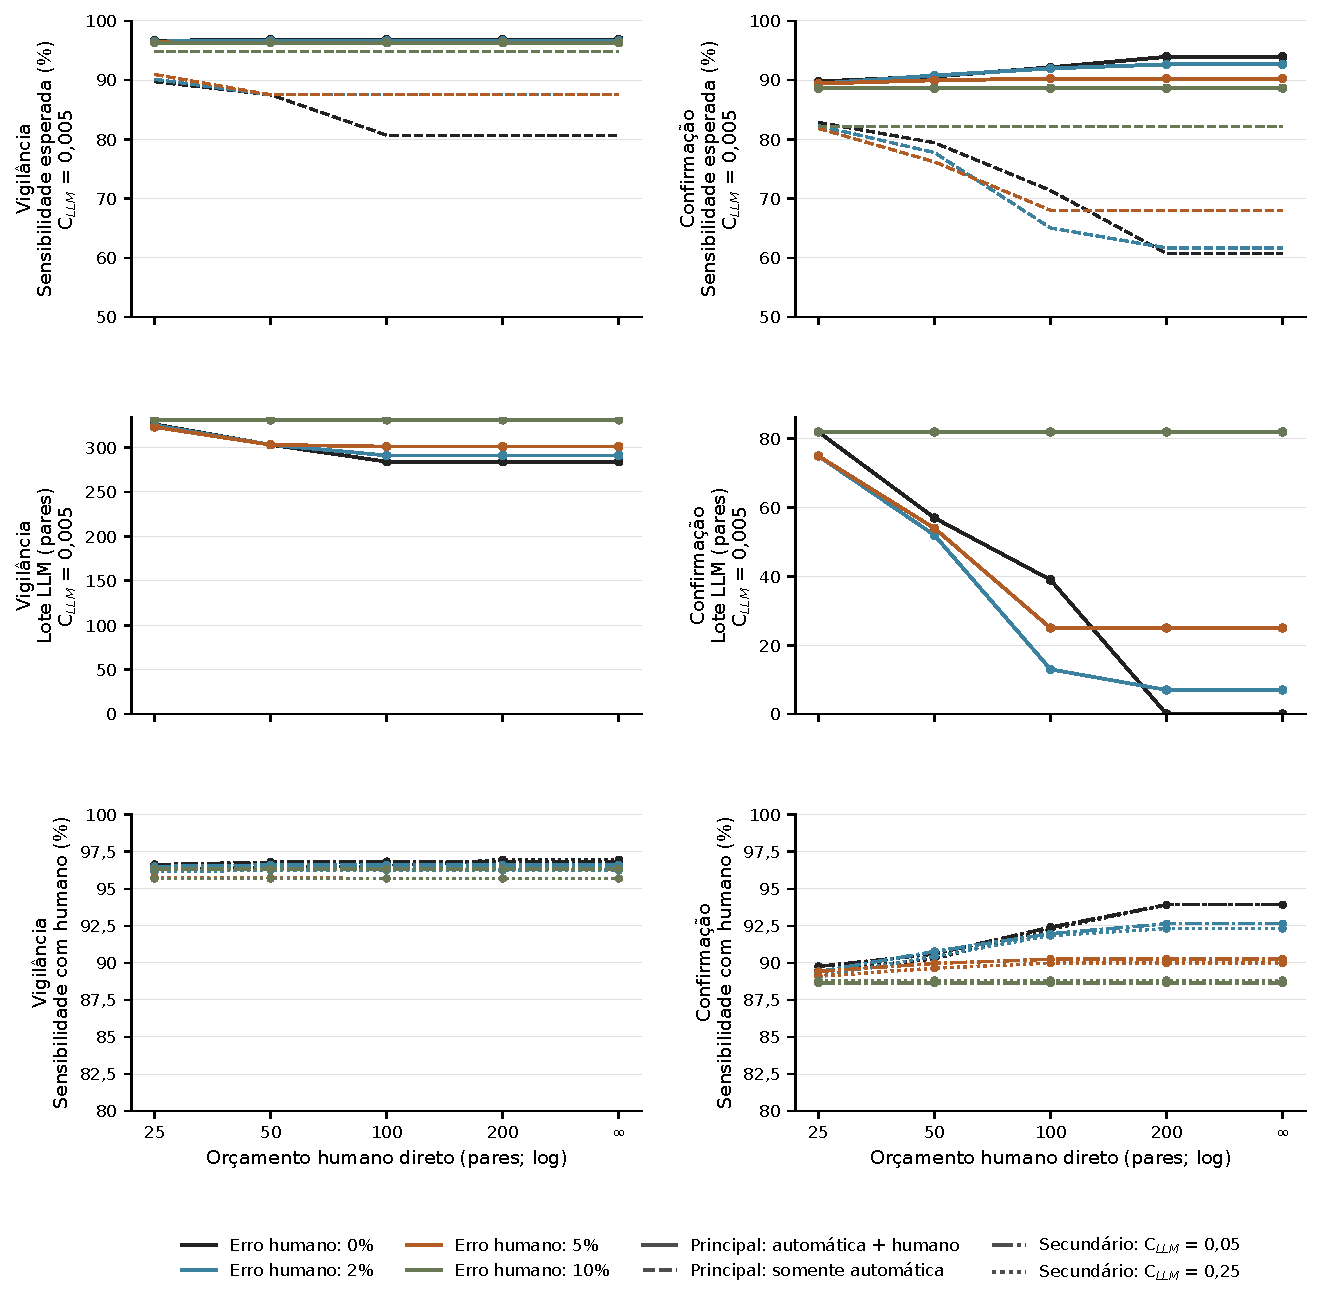
\includegraphics[width=\textwidth,height=0.67\textheight,keepaspectratio]{figures/fig_cap8_varredura_custos.pdf}
\caption{Sensibilidade esperada e volume de revisão segundo orçamento humano direto, custo relativo do LLM e hipótese de erro humano, nos modos vigilância (esquerda) e confirmação (direita). Os painéis superiores distinguem sensibilidade automática e após revisão humana para $C_{LLM}=0{,}005$; os intermediários mostram o lote LLM; os inferiores comparam custos relativos alternativos. As cores representam hipóteses de erro humano, não proporções medidas. Os limites finitos do eixo horizontal estão em escala logarítmica; $\infty$ é categoria de orçamento ilimitado, sem representar um limite de 400 pares. A carga humana adicional de inconclusivos não está incluída no limite direto.}
\label{fig:cap8-varredura-custos}
\end{figure}

Com humanos ilimitados, a comparação de $C_{LLM}=0{,}25$ e erro humano nulo com $C_{LLM}=0{,}005$ e erro humano de 5,0\% alterou, na vigilância, o lote LLM de 212 para 347 pares e a carga humana total esperada de 218,5 para 98,8; a sensibilidade esperada após revisão humana passou de 96,3\% para 95,1\%. Na confirmação, o lote LLM passou de zero para 44 pares, a carga humana esperada de 229,0 para 124,3 e a sensibilidade esperada com revisão humana de 92,3\% para 87,7\%. A perda total esperada passou de 1.208,20 para 1.291,42 na vigilância e de 731,87 para 1.121,49 na confirmação, em revisões humanas equivalentes. Essa comparação, registrada em \texttt{data/varredura\_custos\_antes\_depois.csv}, modifica simultaneamente custo LLM e hipótese de erro humano, não isola o efeito de nenhum deles e não compara as versões históricas completas do motor.

\subsection{Confirmação por restrição de falsos vínculos na base inteira}
\label{sec:e4-np-confirmacao}

A minimização de custo não garante um limite predefinido de falsos vínculos automáticos. Avaliou-se, por isso, uma alternativa denominada NP na implementação, que ordena os candidatos a vínculo por $p$ decrescente e escolhe o prefixo com maior número esperado de vínculos, sujeito a
\[
\sum_{i\in\mathcal{M}}(1-p_i)\leq\alpha\,|\mathcal{M}|,
\]
em que $\mathcal{M}$ inclui obrigatoriamente os vínculos das guardas e os demais vínculos automáticos. A restrição controla a fração esperada de falsos vínculos entre decisões de vínculo, e não $P(\texttt{MATCH}\mid\text{não-vínculo})$ do teste clássico de Neyman e Pearson. A denominação NP identifica a política por restrição, sem implicar garantia frequentista para a proporção de falsos positivos.

Para não-vínculo automático fora das guardas, exigiu-se $p\leq0{,}02$; o restante foi encaminhado ao LLM apenas quando sua perda era inferior à humana e havia orçamento, ou ao revisor humano nos demais casos. Não se permitiu decisão automática fora dos conjuntos admitidos pela restrição. Capacidade humana insuficiente torna o cenário inviável, assim como uma restrição incompatível com as guardas, sem atribuição de métricas iguais a zero aos cenários sem solução.

Os alvos de 0,1\% e 0,2\% foram inviáveis com as guardas mantidas. Embora seus 63 vínculos não tenham apresentado falsos positivos observados, a soma de $1-p$ nesse conjunto foi de 0,67 falso positivo esperado. Mesmo acrescentando os 47 candidatos mais favoráveis, com $p=1$, o limite mínimo foi de 0,61\%, entre 110 vínculos automáticos. A Figura~\ref{fig:cap8-np-confirmacao} distingue essa região inviável dos pontos avaliáveis. O risco esperado não pode ser substituído pela ausência de erro observado no extrato, e seu controle depende da calibração absoluta: a sobreconfiança examinada nas Seções~\ref{sec:e4-classificador-oof} e~\ref{sec:e4-calibracao-beta} pode subestimar $1-p$.

\begin{figure}[!htbp]
\centering
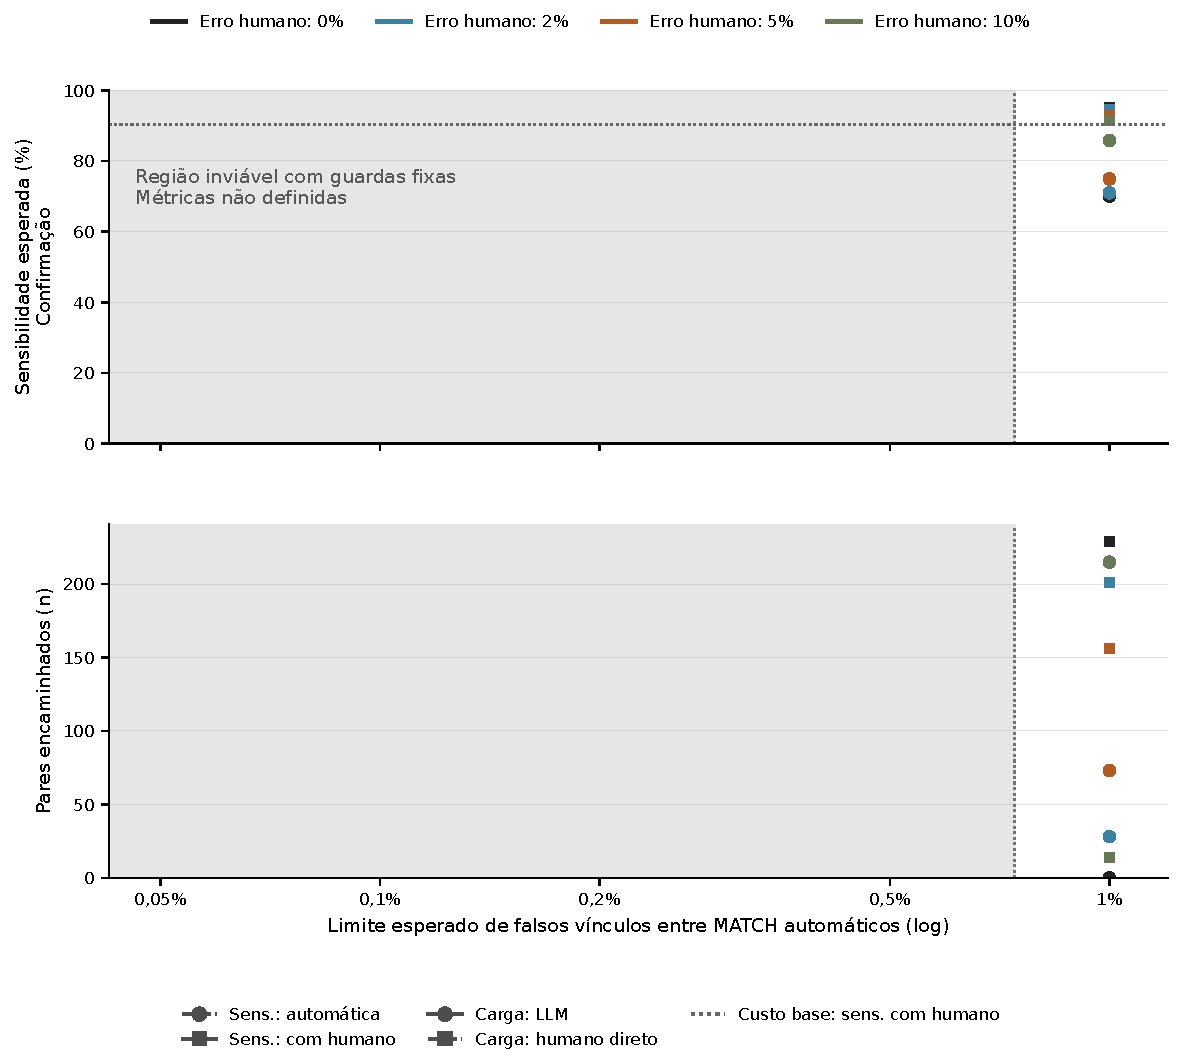
\includegraphics[width=\textwidth,height=0.60\textheight,keepaspectratio]{figures/fig_cap8_np_confirmacao.pdf}
\caption{Política por restrição na confirmação: sensibilidade esperada (painel superior) e encaminhamentos a LLM e revisor humano direto (inferior), segundo o limite da fração esperada de falsos vínculos entre vínculos automáticos, incluindo guardas. As cores representam hipóteses de erro humano; a linha pontilhada indica a sensibilidade com humano da política por custo no cenário-base. O sombreado identifica limites inviáveis com as guardas fixas, sem interpolação de métricas nessa região. As projeções dependem das probabilidades OOF e das proporções do revisor de referência, não constituindo resultados observados de revisão.}
\label{fig:cap8-np-confirmacao}
\end{figure}

O limite de 1,0\% foi viável com orçamento humano ilimitado, mas exigiu mais revisão e maior \textit{expected loss} que a política por custo (Tabela~\ref{tab:cap8-np-confirmacao}). A sensibilidade esperada com revisão humana aumentou de 87,7\% para 90,1\%, enquanto a carga humana total esperada passou de 124,3 para 247,0 pares. O limite incide apenas sobre vínculos automáticos do motor, não sobre falsos positivos de toda a cadeia: estes incluem erros do LLM e do revisor humano. Os valores foram extraídos de \texttt{data/comparacao\_np\_confirmacao.csv} e \texttt{data/np\_confirmacao\_relatorio.md} \cite{Jardim2026phdrepo}.

\begin{table}[!htbp]
\centering
\caption{Confirmação por custo e por restrição NP (limite da fração esperada de falsos vínculos entre os automáticos) de 1,0\%, com $C_{LLM}=0{,}005$, erro humano hipotético de 5,0\% e orçamento humano ilimitado. Sensibilidades, carga adicional após LLM, falsos positivos e perdas são expectativas, não resultados observados da cadeia.}
\label{tab:cap8-np-confirmacao}
\begin{tabular}{lrr}
\hline
Indicador & Custo & NP 1,0\% \\
\hline
Pares selecionados para LLM & 44 & 108 \\
Encaminhamentos humanos diretos & 121 & 241 \\
Carga humana total esperada & 124,3 & 247,0 \\
Sensibilidade automática esperada (\%) & 55,7 & 62,7 \\
Sensibilidade esperada com humano (\%) & 87,7 & 90,1 \\
FP esperados nos vínculos automáticos, com guardas & 0,83 & 1,29 \\
FP esperados na cadeia completa & 2,88 & 10,96 \\
Perda esperada (revisões humanas equivalentes) & 1.121,49 & 1.859,28 \\
\hline
\end{tabular}
\end{table}

\subsection{Fluxo operacional da versão v3}
\label{sec:e4-fluxo}

O fluxo histórico da versão v3 do GZ-CMD, formalizado como desenho avaliado no Algoritmo \ref{alg:gzcmd-pipeline} (Apêndice \ref{apendice:gzcmd}), era composto pelas etapas abaixo; a política v3.1 consta do Algoritmo~\ref{alg:gzcmd-v31}. A classificação OOF e as quatro ações da v3.1 substituem os ajustes e a triagem históricos conforme as Seções~\ref{sec:e4-classificador-oof} e~\ref{sec:e4-politica-v31}.

\begin{enumerate}
\item \textbf{Representação}: cada potencial par era codificado como vetor de 29 subescores do Comparador de Registros, opcionalmente acrescido das medidas contínuas MACD.
\item \textbf{Classificação}: o desenho previa modelo supervisionado (XGBoost ou Random Forest) para produzir escore bruto $s$; a probabilidade efetivamente usada no funil histórico foi a transformação da nota por \textit{Platt scaling}, não a probabilidade multivariada OOF da v3.1.
\item \textbf{Calibração}: os conjuntos $A^+$ e $A^-$ definiam a alternativa de ajuste sigmoide por âncoras, cuja calibração absoluta não estava garantida; essa alternativa distingue-se do \textit{Platt scaling} supervisionado da nota empregado na execução histórica.
\item \textbf{Atribuição de faixa}: a nota final do CdR, distinta do escore do ORL, posicionava o par em uma das seis faixas operacionais (\texttt{low}, \texttt{grey\_low}, \texttt{grey\_mid}, \texttt{grey\_high}, \texttt{near\_high} e \texttt{high}), distintas das três regiões decisórias de $p_{cal}$ (Seção \ref{sec:e4-calibracao}).
\item \textbf{Regras de guarda}: restrições determinísticas podiam forçar decisão ou revisão, independentemente de $p_{cal}$, com as particularidades da execução v3 descritas no início da Seção~\ref{sec:e4-metodo}.
\item \textbf{Triagem por \textit{expected loss}}: calculava-se $EVR(p)$ e a decisão automática de base; a seleção até o limite $L_{max}$ priorizava a revisão forçada por homonímia, depois os limites automáticos de probabilidade e, por último, $EVR>0$, com $EVR$ decrescente dentro de cada prioridade. Guardas determinísticas de aceitação e rejeição não eram candidatas à revisão.
\item \textbf{Revisão assistida}: pares selecionados eram convertidos em dossiê, isto é, um documento estruturado e pseudonimizado contendo os subescores disponíveis do comparador, a probabilidade calibrada, a faixa de confiança atribuída e os códigos das regras de guarda aplicadas. O dossiê era então submetido ao protocolo dual-agente com arbitragem (Seção \ref{sec:e4-revisao-assistida}).
\item \textbf{Decisão final}: a saída era um \textit{label} (\texttt{MATCH}, \texttt{NONMATCH} ou \texttt{UNSURE}) com registro de agente, protocolo e códigos de razão, sem avaliação independente da qualidade dessas justificativas.
\end{enumerate}

\subsection{Revisão clerical assistida}\label{sec:e4-revisao-assistida}

A revisão assistida foi concebida como módulo de apoio, não como substituição do julgamento epidemiológico. O protocolo, descrito a seguir, converte cada par do lote selecionado pelo motor em dossiê estruturado e o submete a dois agentes, com arbitragem por um terceiro em caso de discordância.

\subsection{Protocolo de revisão por modelo de linguagem}\label{sec:e4-protocolo-llm}

O GZ-CMD incorpora revisão assistida por modelo de linguagem para potenciais pares selecionados pelo motor, sem restringir necessariamente o lote à área cinza $[5,9)$ da nota. No estudo-piloto, 517 potenciais pares selecionados pela v3 foram submetidos ao mesmo protocolo, para estimar sensibilidade e especificidade do LLM com \textit{labels} conhecidos, separadamente da decisão da cadeia.

O protocolo adota dois agentes com árbitro. O dossiê JSON contém 14 dos 29 subescores do extrato: três de nome, três de nome da mãe, um de nascimento, seis de endereço e um municipal, este serializado como \texttt{municipality} (Tabela~\ref{tab:dossie-campos}). Não inclui a penalidade por nome comum da mãe, as inversões de data nem os subescores de UF. Reúne também nota final, compostos, indicadores e MACD de nascimento, quando presentes (\path{gzcmd/llm_dossier.py}). A instrução v4 solicita inversão de dia e mês, sexo, UF e datas de evento sem correspondência integral no dossiê; \texttt{PNOME}, \texttt{UNOME} e \texttt{NMAE} não são suas chaves literais. Não se avaliou o efeito dessa incompatibilidade. A execução histórica incluía pseudônimo, probabilidade calibrada, faixa, decisão de base, EVR e guardas, retirando-se as saídas decisórias nas execuções v4. Cada agente emite MATCH, NONMATCH ou UNSURE e confiança autodeclarada, não validada; o consenso é adotado e, na discordância, intervém o árbitro. Não se enviaram campos nominais brutos; os dados permanecem pseudonimizados e sujeitos à Seção~\ref{sec:dados-acesso-etica}. Na v3, o carregador omitiu a política por faixa posterior à separadora do arquivo-base, embora a mensagem de usuário a solicitasse (Apêndice~\ref{sec:apendice-prompts}).\footnote{MACD designa as Medidas Contínuas de Diferença de Datas, atributos derivados do nascimento; EVR é o valor esperado da revisão.}

% Gerada por scripts/dossie_campos_enviados.py; não editar.
\begin{table}[htbp]
\centering\scriptsize
\caption{Subescores do extrato e inclusão no dossiê histórico: 14 de 29.}
\label{tab:dossie-campos}
\begin{tabular}{lll}
\toprule
Campo & Categoria & Enviado \\
\midrule
NOME prim frag igual & nome & sim \\
NOME ult frag igual & nome & sim \\
NOME qtd frag iguais & nome & sim \\
NOME qtd frag raros & nome & não \\
NOME qtd frag comuns & nome & não \\
NOME qtd frag muito parec & nome & não \\
NOME qtd frag abrev & nome & não \\
NOMEMAE prim frag igual & nome da mãe & sim \\
NOMEMAE ult frag igual & nome da mãe & sim \\
NOMEMAE qtd frag iguais & nome da mãe & sim \\
NOMEMAE qtd frag raros & nome da mãe & não \\
NOMEMAE qtd frag comuns & nome da mãe & não \\
NOMEMAE qtd frag muito parec & nome da mãe & não \\
NOMEMAE qtd frag abrev & nome da mãe & não \\
DTNASC dt iguais & nascimento & sim \\
DTNASC dt ap 1digi & nascimento & não \\
DTNASC dt inv dia & nascimento & não \\
DTNASC dt inv mes & nascimento & não \\
DTNASC dt inv ano & nascimento & não \\
CODMUNRES uf igual & município & não \\
CODMUNRES uf prox & município & não \\
CODMUNRES local igual & município & sim \\
CODMUNRES local prox & município & não \\
ENDERECO via igual & endereço & sim \\
ENDERECO via prox & endereço & sim \\
ENDERECO numero igual & endereço & sim \\
ENDERECO compl prox & endereço & sim \\
ENDERECO texto prox & endereço & sim \\
ENDERECO tokens jacc & endereço & sim \\
\bottomrule
\end{tabular}
\par\smallskip\parbox{\linewidth}{\footnotesize Fonte: \path{data/dossie_campos_enviados.csv}, cabeçalho do extrato e auditorias históricas v4 dos dois modos. O escore municipal é enviado como \texttt{municipality}. Compostos, indicadores e nota final não integram os 29 subescores deste quadro.}
\par\footnotesize Dossiê: documento estruturado com os subescores disponíveis para a revisão por modelo de linguagem. CdR: Comparador de Registros.
\end{table}


O modelo utilizado foi o Kimi K2.5 \cite{KimiK2_5_2025}, acessado por meio da API Fireworks AI, na execução de fevereiro de 2026, com temperatura zero e semente fixa (seed=43); o provedor não foi utilizado nas execuções posteriores. Esses parâmetros não garantem repetibilidade integral; os parâmetros e a variabilidade dos revisores posteriores são descritos na Seção~\ref{sec:e4-selecao-llm}. Duas configurações operacionais foram avaliadas: o modo de vigilância, que prioriza a sensibilidade na identificação de vínculos, e o modo de confirmação, que prioriza a precisão das decisões positivas. Os resultados dessa avaliação são apresentados na Seção~\ref{sec:e4-llm-inicial}.

\subsection{Seleção do modelo de linguagem}\label{sec:e4-selecao-llm}

A escolha do modelo considerou concordância com a referência operacional, precisão, sensibilidade, F$_1$, latência média por par e proporção de inconclusivos. O piloto avaliou 517 pares do lote selecionado pelo motor, selecionados para revisão por LLM pela sequência operacional (\textit{pipeline}) v3 (Tabela~\ref{tab:cap8-llm-piloto}). As faixas do piloto, designadas A a D para não se confundirem com as seis faixas operacionais do motor (cujos intervalos são outros), referem-se à nota final do CdR, não ao escore do ORL: faixa A (nota $\geq 3$ e $< 5$; $n=341$), faixa B ($\geq 5$ e $< 7$; $n=133$), faixa C ($\geq 7$ e $< 9$; $n=35$) e faixa D ($\geq 9$; $n=8$). Assim, 341 dos 517 pares (66,0\%) situam-se abaixo da nota 5, fora da área cinza da nota $[5,9)$, que reúne 168 pares (32,5\%); o piloto, portanto, não representa a área cinza da nota, e essa estratificação não a redefine nem altera as faixas do motor nas demais análises. Cinco modelos de linguagem de grande porte foram testados no piloto com \texttt{temperature}=0, \texttt{max\_tokens}=4096, \texttt{top\_p}=1, \texttt{top\_k}=40 e penalidades nulas: Kimi~K2.5 (Moonshot AI), GPT-4o (OpenAI), DeepSeek~V3.2 (DeepSeek; arquitetura \textit{Mixture-of-Experts}), Qwen3-VL-30B (Alibaba; 30 bilhões de parâmetros) e GLM-5 (Zhipu AI). Kimi, DeepSeek, Qwen e GLM foram acessados pela Fireworks AI; GPT-4o, pela API da OpenAI, conforme \path{scripts/pilot_c2_517.py}. Esses fornecedores receberam os dossiês pseudonimizados, não campos nominais brutos, sob as condições da Seção~\ref{sec:dados-acesso-etica}.\footnote{CdR designa o Comparador de Registros.}

{\sloppy Esses parâmetros descrevem o piloto, não todos os revisores posteriores. Na replicação, DeepSeek V4.1 Flash utilizou \texttt{temperature}=0, \texttt{top\_p}=1, \texttt{top\_k}=1 e \texttt{max\_tokens}=800 por chamada, com raciocínio desligado (\path{thinking.type=disabled} e \path{reasoning_effort=none}); Kimi K3 utilizou os mesmos parâmetros de amostragem, \texttt{max\_tokens}=2500 e \path{reasoning_effort=low}. Claude Haiku 5.5 utilizou \texttt{max\_tokens}=2500 por chamada, na configuração padrão do modelo, sem configuração explícita de raciocínio (a API aplica raciocínio adaptativo por padrão; os registros não discriminam tokens de raciocínio) e sem envio de \texttt{temperature}, parâmetro não aceito pelo modelo. Sua geração é estocástica: na ablação do dossiê, a concordância entre controle e execução original foi de 72,2\% (13/18 pares; Seção~\ref{sec:e4-ablacao-dossie}). Mesmo quando aceita, a temperatura zero não garante reprodutibilidade integral entre execuções ou versões do provedor. Os JSONs históricos em \path{data/sprint3b/} registram modelo, execução e resultados, mas não preservam todos os parâmetros de geração; os valores acima estão documentados nos \textit{scripts} \path{run_exp2_opencode_go.py} e \path{run_exp2_anthropic.py} \cite{Jardim2026phdrepo}.\par}

\begin{table}[!ht]
\centering
\caption{Avaliação comparativa de modelos para revisão assistida ($n=517$ pares do lote selecionado pelo motor; intervalos de Wilson, 95\%).}
\label{tab:cap8-llm-piloto}
\resizebox{\textwidth}{!}{%
\begin{tabular}{|l|c|c|c|c|c|c|c|}
\hline
Modelo & Válidos$^a$ & Concordância (\%) & Precisão & Sensibilidade & F$_1$ & Inconcl.\,(\%) & Latência (s/par) \\
\hline
Kimi K2.5      & 499 & 97,8\,[96,1;\,98,8] & 0,909 & 0,789 & \textbf{0,845} & 3,5  & 7,3 \\
\hline
GPT-4o         & 508 & 95,5\,[93,3;\,97,0] & 1,000 & 0,343 & 0,511          & 1,7  & 6,3 \\
\hline
DeepSeek V3.2  & 232 & 93,5\,[89,6;\,96,0] & 0,615 & 0,762 & 0,681          & 55,1 & 54,0 \\
\hline
Qwen3-VL-30B   & 509 & 94,9\,[92,6;\,96,5] & 1,000 & 0,333 & 0,500          & 1,6  & 7,5 \\
\hline
GLM-5           & 212 & 95,3\,[91,5;\,97,4] & 0,769 & 0,833 & 0,800          & 59,0 & 57,6 \\
\hline
\multicolumn{8}{l}{\footnotesize $^a$\,Pares com decisão \texttt{MATCH}/\texttt{NONMATCH}; excluídos os \texttt{UNSURE}.} \\
\end{tabular}%
}
\end{table}

O piloto reuniu $n=517$ pares, mas a concordância exclui inconclusivos e tem denominadores de 212 a 509, conforme a Tabela~\ref{tab:cap8-llm-piloto}. A abstenção seletiva favorece a concordância entre os resolvidos; esses denominadores não são intercambiáveis com os 517 usados como referência no cálculo de poder. Para discriminar com poder de 80\% (nível de significância de 5\%, teste bilateral, aproximação normal para duas proporções independentes, sem correção de continuidade) a concordância de 97,8\%, do Kimi K2.5, de 94,3\%, diferença de 3,5 pontos percentuais, seriam necessários 485 pares por modelo; para uma diferença de 1,5 ponto percentual (97,8\% contra 96,3\%), 1.997 pares por modelo. Como os modelos avaliam os mesmos pares, o cálculo para amostras independentes é conservador, mas não corrige a seleção por abstenção. Os valores foram gerados por \path{scripts/poder_amostral_piloto.py}, com saída em \path{data/poder_amostral_piloto.csv}.

Quatro dos cinco modelos dividiram-se em dois perfis. GPT-4o e Qwen3-VL-30B tiveram precisão de 1,000 e sensibilidade baixa ($\approx$0,34), com omissão de vínculos. DeepSeek~V3.2 e GLM-5 apresentaram proporções de inconclusivos acima de 55\% e latência superior a 54~s/par. Kimi K2.5 \cite{KimiK2_5_2025} teve o maior F$_1$ pontual (0,845), com 3,5\% de inconclusivos e latência de 7,3~s/par, sem superioridade demonstrada em concordância global. Não foi avaliada a correspondência entre códigos de razão, evidência disponível e justificativa produzida; sua emissão no formato solicitado não demonstra qualidade explicativa.

A análise da matriz de confusão por modelo explicita implicações operacionais distintas. O Kimi~K2.5 apresentou 30 verdadeiros positivos, 3 falsos positivos, 8 falsos negativos e 458 verdadeiros negativos entre os 499 pares com decisão válida, configurando equilíbrio entre erros de omissão e comissão compatível com o cenário de vigilância. GPT-4o e Qwen3-VL-30B não produziram falsos positivos, mas omitiram, respectivamente, 23 e 26 dos 41 vínculos presentes na amostra; em contexto de vigilância epidemiológica, esse padrão tenderia a subestimar sistematicamente a mortalidade por tuberculose. DeepSeek~V3.2 e GLM-5 alcançaram distribuição mais equilibrada entre tipos de erro (sensibilidade de 76,2\% e 83,3\%, respectivamente), porém a proporção elevada de inconclusivos reduz o denominador efetivo de avaliação a menos da metade da amostra original e compromete a representatividade das métricas reportadas.

A frequência de arbitragem é indicador complementar. O Kimi~K2.5 teve consenso direto entre os agentes~A e B em 503 dos 517 pares (97,3\%), com uso do árbitro em 14 casos (2,7\%), o que é compatível com sua latência de 7,3~s/par. GPT-4o e Qwen3-VL-30B tiveram 6 arbitragens cada (1,2\%), com concordância entre agentes concentrada na classificação \texttt{NONMATCH}. DeepSeek~V3.2 e GLM-5 acionaram arbitragem em 213 (41,2\%) e 155 (30,0\%) pares, respectivamente, o que indica discordância frequente entre agentes e acompanha latências superiores a 54~s/par. A indução de cadeias de raciocínio (\textit{chain-of-thought}) foi proposta como técnica de elaboração de respostas por etapas \cite{Wei2022chainofthought}. Uma hipótese, não testada no piloto, é que a cadeia de raciocínio estendida tenha levado esses modelos a sinalizar incerteza com mais frequência nesta tarefa; o piloto não isola esse efeito, e a latência maior não veio acompanhada de concordância maior que a do Kimi~K2.5.

Do ponto de vista da validade estatística, os intervalos de Wilson para concordância sobrepõem-se entre os cinco modelos, o que impede rejeitar igualdade ao nível de 95\% de confiança. Ainda assim, o F$_1$ varia de 0,500 (Qwen3-VL-30B) a 0,845 (Kimi~K2.5), diferença de 0,345 que expressa capacidades distintas de identificação de vínculos. Essa aparente contradição, com concordância estatisticamente indistinguível e F$_1$ substancialmente diferente, decorre do forte desbalanceamento da amostra (476 não-pares contra 41 pares). A concordância global é dominada pelos verdadeiros negativos, nos quais todos os modelos exibem desempenho alto, enquanto o F$_1$ pondera explicitamente a detecção da classe minoritária. Essa assimetria reforça a importância de reportar métricas desagregadas por classe em cenários de forte desbalanceamento.

\subsection{Arranjo sequencial com registro interno}\label{sec:e4-arranjo-metodo}

O Algoritmo~\ref{alg:gzcmd-arranjo} descreve a preservação das aceitações do corte e o processamento dos potenciais pares abaixo dele.

O corte do OpenRecLink é específico por passo e separa os vínculos PAR~=~1 dos demais (Seção~\ref{sec:padrao-ouro}). A região abaixo dele contém 61.485 candidatos, dos quais 36 são vínculos PAR~=~2; candidatos não são revisões observadas. A avaliação distingue simulação sem API (S1), chamadas ao LLM (S2) e avaliação com os \textit{labels} (S3). O braço \textit{a posteriori} preserva o corte e aplica a cascata publicada abaixo dele, sem recalibração. Houve registro interno versionado antes da S3, com intervalo de aproximadamente 49 minutos, mas o resultado desse braço já era conhecido e o código originalmente registrado está ausente do histórico do git. Esse registro delimita as escolhas declaradas, sem transformar a avaliação em confirmatória.\footnote{Registro \texttt{8c16a41}, em 5 de novembro de 2026, às 01:22:17 UTC; S3 às 02:11:52 UTC, conforme \path{data/arranjo_corte_metadata.json} na versão \texttt{16d5876}, não no JSON atual. Esse último \textit{commit} consta no histórico às 02:17:13 UTC. O código incorporado posteriormente não corresponde aos bytes inicialmente registrados; a reprodução da S1 requer a versão documentada nos desvios.} O conhecimento prévio do resultado do braço \textit{a posteriori} impede tratar a escolha do enquadramento sequencial como protegida pelo registro \cite{Jardim2026phdrepo}.

No braço principal P, o XGBoost mantém os 30 atributos, hiperparâmetros e semente 42 do classificador da base inteira, com cinco partições externas e cinco internas agrupadas por REFREC (Seção~\ref{sec:e4-classificador-oof}). O classificador é ajustado em toda a parcela de treinamento. A regressão isotônica é reajustada somente nas probabilidades internas fora da amostra dos potenciais pares de treinamento abaixo do corte, sem acesso aos \textit{labels} da partição externa. O ajuste restrito estima a probabilidade de vínculo entre os candidatos que o corte não aceitou. Mantêm-se guardas, custos e orçamentos da v3.1, aplicando a guarda superior à probabilidade recalibrada. Nenhuma partição teve menos de dez vínculos PAR~=~2 no ajuste da calibração; a substituição prevista por sigmoide não foi acionada (\path{data/arranjo_corte_s1_metadata.json}).

As proporções de erro e de inconclusivos do revisor foram estimadas por validação cruzada nas partições externas, por modo e faixa, usando as três coortes de Claude Haiku 5.5 com instruções v4 e dossiê sem as saídas do motor: lote histórico, complemento por linha e complemento por REFREC (Seção~\ref{sec:e4-reruns}). Foram congeladas antes das chamadas novas, em \path{data/arranjo_corte_taxas_crossfit.csv}, sem realimentação pelas respostas posteriores. As decisões do LLM em P reutilizam majoritariamente as respostas dessas mesmas coortes, que também estimaram as proporções do revisor. Apenas dez potenciais pares pendentes na vigilância e 14 na confirmação, na união $P\cup B1$ (P, arranjo principal recalibrado abaixo do corte; B1, ponte que mantém a probabilidade original e troca apenas as proporções do revisor), receberam chamadas novas, conforme \path{data/arranjo_corte_s1_metadata.json}. Esses números não descrevem P isoladamente. A validação cruzada reduz a dependência, mas não a elimina; a avaliação não é prospectiva. A reutilização exige coincidência de modo, potencial par, modelo, instruções e dossiê; os demais seguem o mesmo protocolo de dois agentes e árbitro.

Os braços de comparação com registro interno anterior à S3 são o corte isolado, o corte seguido de revisão humana integral abaixo dele (cenário) e a cascata v3.1 sobre a base inteira. A ponte B1 mantém a base inteira e a probabilidade original, alterando apenas as proporções do revisor para as estimadas por validação cruzada. Seu contraste com a cascata publicada examina a transferência dessas proporções; não isola o efeito da recalibração abaixo do corte. No registro \texttt{8c16a41}, P-Platt, com \textit{Platt scaling} sobre o logit da probabilidade bruta, constava entre os braços, ao lado de P e B1, e as sensibilidades registradas eram duas: A3, que restringe também o ajuste do classificador ao treinamento abaixo do corte, e P-PAR2-grey, que estima $e_{FN}$ somente com PAR~=~2 e agrupa as quatro faixas da área cinza da nota $[5,9)$. Esta última examina se proporções estimadas nos vínculos não aceitos pelo corte alteram a decisão, sem usar os PAR~=~1, mais fáceis, como referência de erro nessa região. A terceira emenda, às 02:01:57 UTC de 5 de novembro de 2026, cerca de dez minutos antes da S3, autorizou as respostas do suplemento e descreveu P-Platt e A3 como braços de sensibilidade registrados (\path{gzcmd/prereg_arranjo_corte.yaml}, emenda 3). Essa reclassificação de P-Platt é desvio do registro inicial, documentado em \path{gzcmd/M_arranjo_corte_desvios.md}; o tratamento de P-Platt como sensibilidade que não substitui P decorre dela, não do registro \texttt{8c16a41}.

A primeira emenda introduziu os alvos suavizados de \citeonline{Platt1999} e otimização com controle de passo, pois o método de Newton saturou na primeira partição. A segunda explicitou as \textit{threads} (número de processos paralelos) necessárias para reproduzir as probabilidades originais fora da amostra. O suplemento autorizou respostas adicionais para P-Platt e A3, sem alterar braços ou custos, mas desviou da proibição inicial de chamadas de sensibilidade. A regra de parada previa mais de 500 potenciais pares pendentes em $P\cup B1$ ou custo novo superior a US\$~2. Foram 24 potenciais pares; US\$~0,076 era a estimativa usada na regra de parada (\path{data/arranjo_corte_s1_metadata.json}), não consumo observado. O consumo tarifado observado foi de US\$~0,063, somando US\$~0,0281 na vigilância e US\$~0,0348 na confirmação. Com US\$~0,1819 dos 69 potenciais pares do suplemento, em 147 chamadas, sendo US\$~0,1754 na vigilância e US\$~0,0066 na confirmação (\path{data/sprint3b/anthropic_sem_mo_v4_arranjo_corte_supl/execucao.json}), o total foi de US\$~0,2448, soma desse valor com os US\$~0,063 das respostas novas (\path{data/arranjo_corte_metadata.json}, campo \texttt{cost\_sources}). A regra de parada não foi acionada \cite{Jardim2026phdrepo}.

O desfecho primário particiona os 36 vínculos PAR~=~2 em aceitos, encaminhados ao humano e perdidos por não-vínculo, com intervalos de Wilson de 95\%. Por modo, contabilizam-se aceitação automática, falsos positivos (FP), encaminhamentos humanos, lote LLM e custo, na base inteira e na área cinza da nota. A sensibilidade após revisão humana, $(V_A+0{,}95V_H)/247$, soma os vínculos aceitos aos encaminhados ponderados pela sensibilidade humana hipotética e divide pelo total de vínculos; é um cenário projetado. Os intervalos são descritivos, sem corrigir dependência entre potenciais pares ou vieses da referência operacional, e as decisões humanas permanecem sem observação. O registro listou esses desfechos sem hipótese direcional nem critério de sucesso (\path{gzcmd/prereg_arranjo_corte.yaml}, campo \texttt{primary\_outcomes\_S3\_only}). A referência do processo de \textit{linkage} de origem recupera os 36 PAR~=~2 por definição do \textit{label}, de modo que ler as perdas de P frente a ela como resultado negativo é interpretação posterior à S3, não teste previsto no registro.

A análise de estabilidade teve registro interno próprio\footnote{Registro versionado em \texttt{3ade1c7}, \path{gzcmd/prereg_robustez_arranjo.yaml}.} e é análise não confirmatória. Esse registro, de 5 de novembro de 2026 às 06:19:04 UTC, é posterior à S3: o critério de dominância de Pareto, com o limiar de 18/20 descrito a seguir, foi fixado quando a dominância de P-Platt na avaliação original já era conhecida. O bloco numérico mantém as partições e varia a semente do XGBoost e o número de processos paralelos; o bloco de partição varia as partições, mantendo semente do classificador e número de processos paralelos. Cada bloco contém 20 réplicas. As proporções do revisor são estimadas nas coortes congeladas, e respostas novas não as realimentam. A dominância de P-Platt exige não piorar vínculos aceitos, FP abaixo do corte, perdidos e encaminhamentos ao humano e ao LLM, com ao menos uma melhora. O critério registrado de estabilidade exige pelo menos 18/20 em ambos os blocos e dominância inversa em no máximo 1/20. Menos de 10/20 em ambos os blocos, ou dominância inversa em pelo menos 10,0\% em algum bloco, classifica a dominância como não sustentada. As respostas do LLM são compartilhadas entre réplicas. Mede-se estabilidade nos mesmos dados, não generalização nem variabilidade amostral \cite{Jardim2026phdrepo}.

\subsection{Análises exploratórias posteriores ao registro}\label{sec:e4-exploratorias-metodo}

{\sloppy
As análises desta subseção são exploratórias e \textit{post hoc}, não substituem o braço P nem corrigem os vieses da referência. A comparação na mesma carga preserva o corte e ordena os candidatos abaixo dele pelo escore do OpenRecLink (O1), pela nota do CdR (O2), pela probabilidade isotônica OOF da base inteira (O3) ou pela probabilidade recalibrada de P (O4). Para os primeiros $k$ candidatos de cada fila, calcula-se a recuperação com revisor humano perfeito e, separadamente, sob omissão humana de 5\%; os artefatos são \path{data/comparador_mesma_carga.csv}, \path{data/comparador_mesma_carga_curva.csv} e \path{data/comparador_mesma_carga_erro05.csv}. A variante de P com decisões \texttt{MATCH} do LLM encaminhadas ao humano contabiliza a carga adicional sem imputar aceitação independente ao LLM (\path{data/comparador_p_match_humano.csv}). A conversão de esforço usa 20 minutos por par e o cenário de 2.156 revisões, não tempos ou carga observados no serviço (\path{data/esforco_arranjo.csv}). A comparação de custos em revisões humanas equivalentes combina carga humana, pares LLM e FP nas unidades da política, mantendo o caráter exploratório e o revisor perfeito (\path{scripts/banca_c_agregados.py}, \path{data/custos_equivalentes_exploratorios.csv}).\footnote{P é o arranjo principal com calibração isotônica abaixo do corte; CdR designa o Comparador de Registros.}

\par}

Os cenários de sensibilidade humana aplicam $s=0{,}95$, $0{,}99$ e $1{,}00$ aos vínculos encaminhados, com especificidade perfeita e sem decisões humanas observadas (\path{data/cenarios_sensibilidade_humana.csv}). O filtro LLM descarta somente \texttt{NONMATCH} e encaminha \texttt{MATCH} e \texttt{UNSURE} ao humano. Seu protocolo interno foi fixado antes dos desfechos, em \path{gzcmd/protocolo_filtro_llm.yaml} (\texttt{488af95}), com emenda \texttt{c931703} autorizando 83 pares novos para completar a cobertura até $k=125$ nos dois modos. A mistura de respostas antigas e novas de modelo estocástico, sem realimentar as proporções do revisor ou outros braços, não constitui validação prospectiva independente (\path{data/filtro_llm_metadata.json}). Avaliam-se somente os orçamentos com cobertura completa; o topo de 440 pares não teve todas as respostas e não fundamenta recuperação projetada.

A subamostragem reduz apenas os negativos do treinamento, mantendo a prevalência original na avaliação e na calibração isotônica (\path{gzcmd/subamostragem.py}, \path{data/subamostragem_treino_resumo.csv}). A correção analítica de prevalência segue a equação (9) de \citeonline{DalPozzolo2015calibrating}; sua aplicação à isotônica já ajustada à prevalência original é diagnóstico de dupla correção, não ajuste recomendado. As análises de carga abaixo do corte, VPP do LLM e mecanismos de perda também foram produzidas após a avaliação com os \textit{labels}, conforme \path{gzcmd/M_arranjo_corte_desvios.md}; sua descrição não altera os números registrados \cite{Jardim2026phdrepo}.

\section{Resultados}\label{sec:e4-resultados}

\subsection{Experimento 1: ablação e impacto das medidas contínuas}
\label{sec:e4-exp1}

A Tabela \ref{tab:cap8-ablacao} apresenta os resultados de ablação com e sem MACD, com os valores das tabelas da Seção~\ref{sec:apendice-ablacao}, organizados por modo operacional.\footnote{MACD designa as Medidas Contínuas de Diferença de Datas, atributos derivados do nascimento.}

\begin{table}[!ht]
\centering
\caption{Ablação restrita aos subescores e à nota final (média $\pm$ desvio-padrão, cinco divisões por COMPREC, registro do Sinan). MACD ON e OFF indicam as Medidas Contínuas de Diferença de Datas de nascimento ativadas ou desativadas. Revisões são contagens absolutas por partição de teste. As métricas são esperadas com proporções de erro do revisor fixadas na configuração v3 (política histórica de três ações: vínculo, não vínculo e revisão por modelo de linguagem), não estimadas de respostas de modelo de linguagem.}
\label{tab:cap8-ablacao}
\resizebox{\textwidth}{!}{%
\begin{tabular}{|l|l|c|c|c|c|c|c|}
\hline
Modo & Configuração & Precisão & Sensibilidade & F$_1$ & F$_{0{,}5}$ & F$_2$ & Revisões \\
\hline
Confirmação & MACD OFF & $0,901\pm0,033$ & $0,910\pm0,012$ & $0,905\pm0,013$ & $0,902\pm0,025$ & n.a. & $215,4\pm30,2$ \\
\hline
Confirmação & MACD ON & $0,951\pm0,004$ & $0,885\pm0,030$ & $0,916\pm0,014$ & $0,937\pm0,004$ & n.a. & $140,6\pm10,0$ \\
\hline
Vigilância & MACD OFF & $0,857\pm0,052$ & $0,936\pm0,008$ & $0,894\pm0,030$ & n.a. & $0,919\pm0,015$ & $244,2\pm43,9$ \\
\hline
Vigilância & MACD ON & $0,945\pm0,006$ & $0,938\pm0,020$ & $0,941\pm0,008$ & n.a. & $0,939\pm0,015$ & $110,0\pm7,1$ \\
\hline
\end{tabular}%
}
\par\footnotesize Fonte: \path{data/ablation_comprec_macd_allowlist_summary.csv} e \path{data/ablation_comprec_nomacd_allowlist_summary.csv}; rodadas na Seção~\ref{sec:apendice-ablacao}.
\end{table}

O experimento saneado utilizou Random Forest com 200 árvores, profundidade máxima 10 e pesos balanceados, calibrado por sigmoide em validação cruzada interna de cinco partições e ajustado somente no treinamento por COMPREC, com 30\% para teste e sementes de divisão de 42 a 46. A semente do classificador permaneceu 42. Os atributos foram restritos aos 29 subescores e à nota final, acrescidos das nove MACD no braço ativado. Mantiveram-se a política v3 e as proporções de erro do revisor fixadas por faixa na configuração, não estimadas; o F$_1$ é esperado, sem chamada a modelo de linguagem. O procedimento, os parâmetros e a lista de atributos estão em \path{data/ablation_comprec_allowlist_metadata.json}; as rodadas, em \path{data/ablation_comprec_macd_allowlist.csv} e \path{data/ablation_comprec_nomacd_allowlist.csv}.\footnote{v3 identifica a política histórica de três ações ou, nas instruções do LLM, a versão que solicita as saídas do motor.}

Com MACD, o F$_1$ esperado foi de 0,941 na vigilância e de 0,916 na confirmação, contra 0,894 e 0,905 sem MACD. As revisões diminuíram 55,0\% e 34,7\%, respectivamente, calculadas como $100(1-\bar n_{ON}/\bar n_{OFF})$, ou 134,2 e 74,8 por partição. Nos testes t pareados, a diferença de F$_1$ apresentou $t(4)=3{,}68$, $p=0{,}021$ na vigilância e $t(4)=0{,}99$, $p=0{,}377$ na confirmação; os testes de Welch, apenas para comparação, deram $t=3{,}41$, $p=0{,}022$ e $t=1{,}32$, $p=0{,}223$. Para revisões, os valores pareados foram $p=0{,}0016$ e $p=0{,}0031$; para precisão, $p=0{,}016$ e $p=0{,}019$; para sensibilidade, $p=0{,}776$ e $p=0{,}056$. São oito comparações exploratórias, sem ajuste de multiplicidade, produzidas por \path{scripts/exp1_testes_t.py} em \path{data/exp1_testes_t_allowlist.csv}. As cinco partições de teste se sobrepõem; o teste t pareado supõe rodadas independentes e tende a produzir valores de $p$ otimistas, que não sustentam inferência de cinco amostras independentes.

A versão anterior selecionava todas as colunas numéricas do extrato não excluídas por nome, inclusive o escore do OpenRecLink, que define PAR~=~1 pelo corte de cada passo, a situação de encerramento e identificadores. O F$_1$ esperado de 0,954 na vigilância e as reduções de revisões de 14,5\% e 17,6\%, na vigilância e na confirmação, são resultados desse caminho histórico contaminado, preservados em \path{data/ablation_comprec_macd.csv} e \path{data/ablation_comprec_nomacd.csv}, não os resultados saneados. A comparação consta de \path{data/exp1_vazamento_comparacao.csv}. A mudança não pode ser atribuída somente ao escore do OpenRecLink: a restrição retirou conjuntamente campos brutos, identificadores, atributos duplicados e outros derivados. A seleção saneada tampouco demonstra ausência universal de vazamento, pois a nota e os subescores permanecem relacionados à construção da referência. Esta ablação mantém a v3; não foi refeita com a política v3.1 nem com o dossiê sem as saídas do motor. Com a mesma política v3, mas com Claude Haiku 5.5, instruções v4 e dossiê sem as saídas do motor, a cascata sobre a base inteira perdeu 91 vínculos por decisão de não vínculo (\texttt{NONMATCH}) na vigilância, com sensibilidade automática de 58,3\% (Tabela~\ref{tab:cap8-referencia}).\footnote{v3.1 identifica a política de quatro ações, com revisão humana distinta da revisão LLM; v4 identifica as instruções do LLM sem solicitação das saídas do motor.}

\subsection{Experimento 2: desempenho da revisão assistida}
\label{sec:e4-exp2}

O resultado histórico do Experimento 2 corresponde à execução de fevereiro de 2026 com Kimi K2.5, instruções v3 e dossiê completo, incluindo as saídas decisórias do motor. O lote de 1.410 potenciais pares foi selecionado pela política v3, não corresponde à totalidade da área cinza da nota e inclui 22 pares com nota final do CdR $v\geq9$. A Tabela~\ref{tab:cap8-revisao-desempenho} apresenta a matriz reconstruída contra a referência operacional, separando esse estrato dos pares com $v<9$, para não atribuir à região de maior ambiguidade a sensibilidade obtida entre os pares de nota elevada \cite{Jardim2026phdrepo}.\footnote{CdR designa o Comparador de Registros.}

\begin{table}[!ht]
\centering
\caption{Resultado histórico observado do Kimi K2.5 no Experimento 2 (Exp2, revisão assistida), por nota final $v$ do Comparador de Registros (CdR), com dossiê completo (incluindo as saídas decisórias do motor) e instruções v3 (versão histórica que solicita essas saídas), em fevereiro de 2026.}
\label{tab:cap8-revisao-desempenho}
\begin{tabular}{lrrrrrrr}
\hline
Nota & $N$ & VP & FP & FN & VN & Inconcl. & Vínculos inconcl. \\
\hline
$v<9$ & 1.388 & 57 & 6 & 19 & 1.265 & 41 & 6 \\
$v\geq9$ & 22 & 22 & 0 & 0 & 0 & 0 & 0 \\
Total & 1.410 & 79 & 6 & 19 & 1.265 & 41 & 6 \\
\hline
\end{tabular}%
\par\smallskip
\parbox{\linewidth}{\footnotesize VP: verdadeiros positivos; FP: falsos positivos; FN: falsos negativos; VN: verdadeiros negativos. Os inconclusivos são apresentados separadamente, sem integrar a matriz dos resolvidos. Fonte: \texttt{data/exp2\_gabarito\_reconstruido.csv} e \texttt{data/exp2\_reruns\_por\_banda.csv} \cite{Jardim2026phdrepo}.}
\end{table}

Os valores foram reconstruídos pelo \textit{script} \path{scripts/reconstruir_gabarito_exp2.py}, mediante cruzamento com a referência operacional por \texttt{pair\_id}, pseudônimo determinístico calculado pelo SHA-256 da concatenação de \texttt{COMPREC}, \texttt{REFREC} e \texttt{PASSO}, sem sal e truncado nos primeiros 16 caracteres hexadecimais. Quem dispõe dos identificadores internos pode recalculá-lo, de modo que o procedimento não garante anonimização irreversível. As classificações por potencial par depositadas no Zenodo (Seção~\ref{sec:concl-contribuicoes}) e o \texttt{pair\_id} permanecem pseudonimizados para o laboratório, que dispõe da informação adicional necessária à associação com registros nominais. O depósito tem acesso restrito, mediante solicitação e acordo de uso, sob as condições éticas da Seção~\ref{sec:dados-acesso-etica}; somente agregados são públicos. Seu inventário histórico reúne resultados da cascata sobre a base inteira e da v3.1, não os resultados atuais do arranjo. A versão 3.0.1 corrige documentação e metadados sem alterar os resultados experimentais da versão 3.0.0, inclui o frame individual de equidade no conteúdo restrito e distingue medidas de k-anonimidade de uma garantia de anonimização (Seção~\ref{sec:ambiente-computacional}) \cite{Jardim2026zenodoGzcmd,Jardim2026zenodoGzcmd301}. Entre os 1.369 pares resolvidos, a sensibilidade observada foi de 80,6\% e a precisão de 92,9\%; no estrato $v<9$, a sensibilidade foi de 75,0\%, contra 100,0\% nos 22 vínculos com $v\geq9$. Dos 104 vínculos do lote, 19 receberam decisão de não-vínculo e 6 permaneceram entre os 41 inconclusivos. A presença das saídas do motor no dossiê condiciona a interpretação desse resultado histórico: a ancoragem nessas informações foi examinada na Seção~\ref{sec:e4-ablacao-dossie}, sem pressupor independência entre revisão e triagem \cite{Jardim2026phdrepo}.

A exportação restrita com identificador por HMAC-SHA256, descrita na Seção~\ref{sec:export-restrita}, destina-se a novas exportações e não modifica os identificadores nem os resultados históricos apresentados acima.

\subsection{Revisão assistida por modelo de linguagem: execução inicial}\label{sec:e4-llm-inicial}

A cascata de filtragem descrita neste capítulo reduz o universo de potenciais pares a um subconjunto residual de decisão ambígua. Na versão v3 do GZ-CMD, o lote de 1.410 pares da vigilância foi selecionado pelo valor esperado da revisão (EVR), pelos limites automáticos de probabilidade e pela regra de homonímia, com as prioridades descritas na Seção~\ref{sec:e4-motor-politica}, e não por um critério de consenso entre classificadores.
Nesse estrato, a inclusão de um modelo de linguagem de grande escala (\textit{Large Language Model}, LLM) como revisor complementar permite avaliar dossiês estruturados dos potenciais pares.

O protocolo experimental, incluindo o modelo utilizado, a estrutura do dossiê e o mecanismo de duplo agente com árbitro, é descrito na Seção~\ref{sec:e4-protocolo-llm}.
A proporção de consenso entre os dois agentes primários alcançou 97{,}2\% no modo vigilância e 94{,}7\% no modo confirmação, o que mede concordância entre agentes, não acerto frente à referência operacional.

% Gerada por scripts/banca_c_agregados.py; não editar manualmente.
\begin{table}[htbp]
\centering
\small
\caption{Matrizes de confusão da execução anterior de Kimi K2.5, por modo de operação (15 de fevereiro de 2026).}
\label{tab:qw2-confusion}
\begin{tabular}{llrrrl}
\toprule
Modo & Classe real & MATCH & NONMATCH & Total & Protocolo \\
\midrule
Vigil\^ancia & Par verdadeiro & 72 & 32 & 104 & consenso: 1.371; \'arbitro: 39 \\
Vigil\^ancia & N\~ao par & 6 & 1.300 & 1.306 & -- \\ \midrule
Confirma\c{c}\~ao & Par verdadeiro & 91 & 10 & 101 & consenso: 412; \'arbitro: 23 \\
Confirma\c{c}\~ao & N\~ao par & 3 & 331 & 334 & -- \\
\bottomrule
\end{tabular}
\par\smallskip\parbox{\linewidth}{\footnotesize Fonte: \path{data/qw2_kimi_agregado.csv}, gerado de JSONs privados por \path{scripts/banca_c_agregados.py}, com hash de cada fonte e sem dados por par. A vigilância é execução anterior, distinta da matriz reconstruída da Tabela~\ref{tab:cap8-revisao-desempenho}. Comparações entre revisores: Tabela~\ref{tab:cap8-reruns}.}
\end{table}


Os resultados indicam desempenho assimétrico entre os dois modos operacionais (Tabela~\ref{tab:qw2-confusion}).
No modo vigilância, Kimi K2.5 revisou 1.410 pares e obteve precisão de 0{,}923 com sensibilidade de 0{,}692, resultando em $F_1 = 0{,}791$, em execução anterior do mesmo protocolo, de 15 de fevereiro de 2026, registrada no arquivo privado \path{data/qw2/qw2_vigilancia_kimi.json}, com síntese versionada em \path{data/qw2_kimi_agregado.csv}. Essa execução apresentou 72 verdadeiros positivos, 6 falsos positivos, 32 falsos negativos e 1.300 verdadeiros negativos. O agregado foi gerado por \path{scripts/banca_c_agregados.py}, preservando os hashes das fontes e as contagens por modo, sem \texttt{pair\_id}, respostas individuais ou texto livre. Distingue-se da matriz reconstruída a partir de \path{data/sprint3b/exp2_llm_sync_vigilancia.json}, com 79 verdadeiros positivos, 6 falsos positivos, 19 falsos negativos, 1.265 verdadeiros negativos e 41 inconclusivos, apresentada na Tabela~\ref{tab:cap8-revisao-desempenho}. A Tabela~\ref{tab:cap8-reruns} constitui a referência para comparação entre revisores e reavaliações neste capítulo.
A especificidade elevada ($0{,}995$) indica que o modelo raramente classifica pares verdadeiramente negativos como correspondências, comportamento desejável quando o custo de falsos positivos é alto.
Contudo, 32 vínculos foram classificados como não correspondentes, o que representa perda de 30{,}8\% dos positivos nesse estrato residual.
As rejeições devem ser interpretadas à luz da ancoragem nas saídas do motor examinada na Seção~\ref{sec:e4-ablacao-dossie}, em vez de serem atribuídas exclusivamente à ausência de campos textuais brutos.

No modo confirmação, o desempenho difere: sobre 435 pares, a precisão atinge 0{,}968 e a sensibilidade sobe para 0{,}901, elevando o $F_1$ para 0{,}933.
A prevalência de vínculos nesse modo (23{,}2\%) é substancialmente maior do que no modo vigilância (7{,}4\%); a precisão depende dessa prevalência, e os pares de cada modo diferem em composição, o que impede atribuir a diferença entre modos apenas ao revisor.

% Gerada por scripts/banca_c_agregados.py; não editar manualmente.
\begin{table}[htbp]
\centering
\small
\caption{Desempenho de Kimi K2.5 na execução anterior da revisão assistida de pares residuais, por modo de operação.}
\label{tab:qw2-llm-comparison}
\begin{tabular}{lrrrrrr}
\toprule
Modo & $n$ & Precis\~ao & Sensibilidade & $F_1$ & Especif. & Acur\'acia \\
\midrule
Vigil\^ancia & 1.410 & 0,923 & 0,692 & 0,791 & 0,995 & 0,973 \\
Confirma\c{c}\~ao & 435 & 0,968 & 0,901 & 0,933 & 0,991 & 0,970 \\
\bottomrule
\end{tabular}
\par\smallskip\parbox{\linewidth}{\footnotesize Fonte: \path{data/qw2_kimi_agregado.csv}, gerado de JSONs privados por \path{scripts/banca_c_agregados.py}, com hash de cada fonte e sem dados por par. A vigilância é execução anterior, distinta da matriz reconstruída da Tabela~\ref{tab:cap8-revisao-desempenho}. Comparações entre revisores: Tabela~\ref{tab:cap8-reruns}.}
\end{table}


A Tabela~\ref{tab:qw2-llm-comparison} sintetiza as métricas de desempenho nos dois modos.
A diferença de sensibilidade entre os modos ($0{,}692$ \textit{versus} $0{,}901$) descreve lotes de composição distinta e dossiês com saídas do motor (Seção~\ref{sec:e4-ablacao-dossie}). As chamadas são individuais, sem informar a prevalência do lote ao modelo; não se pode atribuir a diferença a uma resposta do revisor à proporção de vínculos.
Esses achados, obtidos com dossiê que incluía as saídas do motor, sugeriram adequação da revisão por LLM à confirmação. Não se mantiveram na cascata sobre a base inteira (Seção~\ref{sec:e4-cascata}), na qual o LLM recebeu poucos potenciais pares da confirmação e a revisão humana concentrou o esforço.
Para o modo vigilância, a perda de sensibilidade demanda cautela e aponta para a necessidade de estratégias complementares, como o encaminhamento ao revisor humano previsto na quarta ação da política v3.1 (Seção~\ref{sec:e4-politica-v31}) ou a inclusão de campos textuais no dossiê.

\subsection{Replicação da revisão assistida com revisores independentes}
\label{sec:e4-revisores}

A replicação com dossiê completo e instruções v3 utilizou DeepSeek V4.1 Flash, via OpenCode Go, com raciocínio desligado e temperatura zero, e Claude Haiku 5.5, via API da Anthropic, sem parâmetro de temperatura. No modo confirmação, Kimi K3, com esforço de raciocínio baixo, completou apenas 343 dos 435 pares, em razão do esgotamento de cota. Esses modelos receberam o mesmo lote e o protocolo de dois agentes com árbitro; a denominação de revisores independentes refere-se às instâncias e aos fornecedores, embora o dossiê contivesse informação decisória prévia. A Tabela~\ref{tab:cap8-revisores} reestratifica os resultados por nota $v<9$ e $v\geq9$. O resultado de Kimi K2.5 na confirmação provém da fonte alternativa QW2 (registro das execuções de revisão por modelo de linguagem) e é identificado separadamente na Tabela~\ref{tab:cap8-reruns}; a equivalência de protocolo com a execução histórica de vigilância permanece por verificar \cite{Jardim2026phdrepo}.

% Fonte: data/exp2_reruns_por_banda.csv, estrato limiar_9, dossiê completo/v3.
\begin{table}[!htbp]
\centering
\caption{Resultados observados dos revisores com dossiê completo e instruções v3, estratificados pela nota final do Comparador de Registros (CdR), $v$.}
\label{tab:cap8-revisores}
\footnotesize
\resizebox{\linewidth}{!}{%
\begin{tabular}{llrrrrrrr}
\hline
Revisor & Nota & $N$ & VP & FP & FN & VN & Inconcl. (pares verdadeiros) & Sens. (\%) \\
\hline
\multicolumn{9}{l}{\textbf{Vigilância}} \\
Kimi K2.5 & $v<9$ & 1.388 & 57 & 6 & 19 & 1.265 & 41 (6) & 75,0 \\
 & $v\geq9$ & 22 & 22 & 0 & 0 & 0 & 0 (0) & 100,0 \\
DeepSeek V4.1 Flash & $v<9$ & 1.388 & 27 & 3 & 42 & 1.256 & 60 (13) & 39,1 \\
 & $v\geq9$ & 22 & 22 & 0 & 0 & 0 & 0 (0) & 100,0 \\
Claude Haiku 5.5 & $v<9$ & 1.388 & 16 & 0 & 10 & 1.103 & 259 (56) & 61,5 \\
 & $v\geq9$ & 22 & 19 & 0 & 0 & 0 & 3 (3) & 100,0 \\
Levanto Sage 2 & $v<9$ & 1.388 & 36 & 9 & 20 & 1.224 & 99 (26) & 64,3 \\
 & $v\geq9$ & 22 & 13 & 0 & 1 & 0 & 8 (8) & 92,9 \\
\hline
\multicolumn{9}{l}{\textbf{Confirmação}} \\
DeepSeek V4.1 Flash & $v<9$ & 377 & 12 & 1 & 8 & 287 & 69 (24) & 60,0 \\
 & $v\geq9$ & 58 & 57 & 1 & 0 & 0 & 0 (0) & 100,0 \\
Claude Haiku 5.5 & $v<9$ & 377 & 6 & 0 & 5 & 203 & 163 (33) & 54,5 \\
 & $v\geq9$ & 58 & 49 & 1 & 0 & 0 & 8 (8) & 100,0 \\
Kimi K3 (parcial) & $v<9$ & 295 & 15 & 2 & 16 & 248 & 14 (9) & 48,4 \\
 & $v\geq9$ & 48 & 42 & 1 & 0 & 0 & 5 (5) & 100,0 \\
\hline
\end{tabular}%
}
\par\smallskip
\parbox{\linewidth}{\footnotesize VP: verdadeiros positivos; FP: falsos positivos; FN: falsos negativos; VN: verdadeiros negativos. Sensibilidade entre resolvidos: $VP/(VP+FN)$; inconclusivos não são acertos. Kimi K3: 343 respostas em 435 pares, sem imputação dos 92 ausentes. Levanto Sage 2 utiliza uma escolha por par, não dois agentes e árbitro; a comparação não isola o efeito do modelo. Fonte: \texttt{data/exp2\_reruns\_por\_banda.csv} \cite{Jardim2026phdrepo}.}
\par\footnotesize Dossiê completo: inclui as saídas decisórias do motor. Instruções v3: solicitam essas saídas. CdR: Comparador de Registros; $v$: sua nota final.
\end{table}


Com \texttt{UNSURE} como terceira categoria, o kappa de Cohen \cite{McHugh2012kappa} entre Kimi K2.5 e DeepSeek V4.1 Flash foi de 0,745 na vigilância; entre Kimi K2.5 e Claude Haiku 5.5, de 0,426; e entre DeepSeek e Haiku, de 0,442. Excluindo os inconclusivos de qualquer revisor, os valores foram, respectivamente, 0,794, 0,985 e 1,000. Na confirmação, DeepSeek e Haiku apresentaram kappa de 0,495 com inconclusivos e 1,000 sem eles; nas comparações parciais com Kimi K3, os valores foram de 0,593 e 0,976 para DeepSeek, e de 0,372 e 0,985 para Haiku. Os denominadores variam com a disponibilidade de respostas e a exclusão de inconclusivos, conforme \texttt{data/exp2\_kappas\_revisores.csv}; a concordância perfeita no subconjunto resolvido não representa concordância em toda a coorte \cite{Jardim2026phdrepo}.

O estrato de nota elevada contribui para a sensibilidade agregada dos revisores. Na vigilância, DeepSeek V4.1 Flash reconheceu os 22 vínculos com $v\geq9$, mas apresentou sensibilidade de 39,1\% nos resolvidos com $v<9$; Claude Haiku 5.5 apresentou, nesse último estrato, sensibilidade de 61,5\%, mantendo 259 inconclusivos. Os erros compartilhados motivaram a ablação apresentada na subseção seguinte, em vez de serem atribuídos exclusivamente à insuficiência dos campos de identificação.

Foi testado também Levanto Sage 2 (\texttt{levanto-sage-2}), modelo de decisão que retorna uma escolha entre vínculo e não-vínculo, com possibilidade de abstenção. Diferentemente dos demais revisores, realizou uma decisão por par, sem o protocolo de dois agentes e árbitro. Na vigilância, com as saídas do motor, apresentou especificidade de 99,3\% e sensibilidade de 70,0\% entre resolvidos; sem essas saídas, produziu 164 falsos positivos e 446 inconclusivos em 1.410 pares, com AUC de 0,82 para a probabilidade de vínculo. A AUC utiliza \texttt{probabilities[match]}, não a confiança na escolha devolvida, cujo alvo muda conforme a classe escolhida. Esses resultados constam de \texttt{data/exp2\_sage\_resumo.csv} e \texttt{data/exp2\_sage\_relatorio.md}; diferenças de protocolo e execuções únicas impedem atribuir o contraste apenas ao modelo \cite{Jardim2026phdrepo}.

\subsection{Ablação do dossiê: mudanças de decisão sem as saídas do motor}
\label{sec:e4-ablacao-dossie}

Os falsos negativos compartilhados pelos três revisores que receberam o mesmo dossiê motivaram a investigação de uma hipótese distinta da insuficiência da evidência de identificação: a apresentação das saídas do motor poderia induzir ancoragem na decisão previamente calculada, reduzindo a independência da revisão assistida. O grupo \texttt{model\_outputs} reúne a probabilidade calibrada (\texttt{p\_cal}), a decisão de base (\texttt{base\_choice}), a faixa de confiança (\texttt{band}), o valor esperado da revisão (\texttt{evr}), a indicação de regra de guarda (\texttt{guardrail}) e sua justificativa (\texttt{guardrail\_reason}). Na calibração histórica, \texttt{p\_cal} é uma função monótona da nota do comparador, enquanto os demais campos também podem transmitir informação sobre a probabilidade ou a decisão do motor, compondo possíveis referências para o julgamento do revisor.

Foram selecionados 18 vínculos que, na vigilância, receberam \texttt{NONMATCH} de pelo menos dois dos três revisores originais; nove foram rejeitados pelos três. Cada potencial par foi submetido ao controle com dossiê completo e ao braço de nome histórico \texttt{sem\_pcal}: a função \texttt{ablate()} retira somente o grupo \texttt{model\_outputs}, preservando os demais campos, inclusive subescores, nota e MACD (\path{scripts/run_exp2_ablacao_dossie.py}). Mantêm-se o prompt original e o protocolo de dois agentes com árbitro; a versão do prompt não está registrada nos JSONs originais nem nos agregados desses braços. A busca nos cinco originais locais, nas seis coortes históricas, inclusive \path{data/sprint3b/anthropic_sem_mo_v4/}, e no histórico do executor não recuperou versão ou hash que certifique o prompt dos braços selecionados. As coortes completas v4 registram versão e hash, sem estabelecer identidade com os braços de 18; os metadados disponíveis e as ausências estão em \path{data/sprint3b/ablacao/ablacao_dossie_proveniencia.json}. DeepSeek V4.1 Flash e Claude Haiku 5.5 completaram ambos; Kimi K3 participou de sondagem em três pares, sem integrar a inferência pareada. As contagens estão em \path{data/ablacao_dossie_agregado.json} e nos checkpoints públicos agregados \path{data/sprint3b/ablacao/*_agregado.json}, sem identificadores individuais \cite{Jardim2026phdrepo}.\footnote{MACD designa as Medidas Contínuas de Diferença de Datas, atributos derivados do nascimento.}

A comparação pareada utilizou o teste de McNemar exato bilateral, tendo como desfecho primário a decisão de vínculo (\texttt{MATCH}) em oposição às demais decisões, sem ajuste de multiplicidade. A passagem de \texttt{NONMATCH} para inconclusivo (\texttt{UNSURE}) foi contabilizada separadamente, pois retira a rejeição explícita do vínculo, mas não constitui reconhecimento correto do vínculo. A Tabela~\ref{tab:cap8-ablacao-dossie} distingue essas transições e apresenta a concordância entre o braço controle e a execução original, que avalia repetibilidade neste subconjunto, não acurácia no lote completo.

% Fontes: data/ablacao_dossie_relatorio.md, data/ablacao_dossie_agregado.json
% e data/sprint3b/ablacao/resumo.json.
\begin{table}[!ht]
\centering
\footnotesize
\caption{Ablação conjunta das saídas do motor no dossiê de revisão, em 18 pares verdadeiros selecionados por falso negativo compartilhado no modo vigilância.}
\label{tab:cap8-ablacao-dossie}
\resizebox{\linewidth}{!}{%
\begin{tabular}{lccrrrc}
\toprule
Modelo & \shortstack{Controle\\M/U/N} & \shortstack{Ablação\\M/U/N} & \shortstack{FN para\\MATCH} & \shortstack{FN para\\UNSURE} & \shortstack{McNemar\\$p$} & \shortstack{Controle =\\original} \\
\midrule
DeepSeek V4.1 Flash & 0/0/18 & 9/9/0 & 9 & 9 & 0,004 & 18/18 \\
Claude Haiku 5.5 & 0/9/9 & 7/11/0 & 2 & 7 & 0,016 & 13/18 \\
\bottomrule
\end{tabular}%
}
\par\smallskip
\parbox{\linewidth}{\footnotesize M: \texttt{MATCH} (vínculo); U: \texttt{UNSURE} (inconclusivo); N: \texttt{NONMATCH} (não aceito como vínculo). FN: falsos negativos do braço controle, não da execução original. Ablação: retirada de todo o grupo \texttt{model\_outputs}. McNemar exato bilateral para \texttt{MATCH} versus demais decisões, sem ajuste de multiplicidade. A mudança para \texttt{UNSURE} não constitui reconhecimento correto do vínculo. Fonte: \texttt{data/sprint3b/ablacao/resumo.json} \cite{Jardim2026phdrepo}.}
\par\footnotesize Ablação: retirada conjunta das saídas decisórias do motor do dossiê, documento estruturado com os subescores disponíveis para a revisão.
\end{table}


Sem as saídas do motor, nenhum dos 18 vínculos foi rejeitado por qualquer dos dois modelos. No DeepSeek V4.1 Flash, os 18 falsos negativos do controle se distribuíram igualmente entre \texttt{MATCH} e \texttt{UNSURE} após a ablação; no Claude Haiku 5.5, dos 9 falsos negativos do controle, 2 passaram a \texttt{MATCH} e 7 a \texttt{UNSURE}. As sete decisões de vínculo do Claude Haiku 5.5 incluem ainda cinco pares classificados como inconclusivos no controle, razão pela qual o teste de McNemar para \texttt{MATCH} não se restringe às duas reversões de falso negativo. O controle reproduziu todas as decisões originais do DeepSeek V4.1 Flash, mas apenas 13 das 18 do Claude Haiku 5.5, documentando variabilidade entre execuções deste último, cuja API não recebeu parâmetro de temperatura.

Os resultados são compatíveis com ancoragem ou abstenção generalizada, sem identificar causalmente esses mecanismos. Nas coortes completas com instruções v4 e sem \texttt{model\_outputs}, DeepSeek V4.1 Flash produziu zero \texttt{NONMATCH} em 1.845 revisões e Claude Haiku 5.5 produziu 1.582 (85,7\%), conforme \path{data/ablacao_dossie_taxa_base.csv}. A unidade é a revisão (modo, potencial par), pois as coortes podem compartilhar pares. Essa proporção de referência é descritiva: os 18 vínculos foram selecionados por erro compartilhado, e a versão do prompt original desses braços permanece não identificada após a busca de proveniência descrita acima. Não há controle negativo com não vínculos. A retirada conjunta de \texttt{model\_outputs} impede separar a contribuição de seus campos, e a nota final, preservada, ainda pode transmitir informação do motor. A manutenção de instruções relativas a campos retirados também pode favorecer inconclusivos. Esses achados motivaram a avaliação seguinte, não uma demonstração de ancoragem.

A avaliação compreende apenas 18 pares, selecionados por erro compartilhado na execução original, e não permite estimar o desempenho da ablação no conjunto dos pares submetidos ao \textit{linkage}, nem seu efeito sobre falsos positivos. O braço controle reproduz esse viés de seleção, pois reapresenta os mesmos pares escolhidos em função do erro, não constituindo amostra independente de avaliação. A comparação informa a mudança de decisão neste subconjunto condicionado ao erro, com variabilidade entre execuções no Claude Haiku 5.5, sem autorizar a generalização da ausência de rejeições aos demais vínculos.

\subsection{Reavaliação sem as saídas do motor}
\label{sec:e4-reruns}

A retirada do grupo \texttt{model\_outputs} foi estendida às coortes históricas completas, preservando subescores, nota final e MACD. Com as instruções v3, que ainda faziam referência a \texttt{p\_cal} e \texttt{band} e cujo envio omitia a política por faixa do arquivo-base (Seção~\ref{sec:e4-protocolo-llm}), Claude Haiku 5.5 produziu 89,2\% de inconclusivos na vigilância, e DeepSeek V4.1 Flash, 86,2\%. Essas proporções descrevem o comportamento de instruções que solicitavam informações ausentes, não uma estimativa isolada da ambiguidade dos campos. Elaborou-se, por isso, a versão v4, com política única de decisão pela evidência disponível: concordância forte de nome e nascimento compatível sustenta vínculo, contradição forte não explicada sustenta não-vínculo, e sinais mistos ou evidência insuficiente justificam inconclusivo. A nota permanece apenas como informação contextual, sem determinar a decisão \cite{Jardim2026phdrepo}.

O protocolo de dois agentes e árbitro e o esquema de resposta foram preservados. A versão e o SHA-256 do arquivo completo de instruções v4 foram registrados nos metadados, conforme \texttt{gzcmd/M4\_prompt\_v4.md}, com \textit{checkpoints} separados por versão. As mesmas instruções foram utilizadas nas coortes de vigilância e confirmação selecionadas pelo motor. A Tabela~\ref{tab:cap8-reruns} reúne resultados históricos e reavaliações, distinguindo dossiê, versão das instruções e execução parcial \cite{Jardim2026phdrepo}.

% Gerada por scripts/avaliar_reruns_exp2.py; fonte: data/exp2_reruns_resumo.csv.
\begin{table}[!ht]
\centering
\footnotesize
\caption{Avaliação dos revisores no Experimento 2 (revisão assistida por LLM), segundo o dossiê (completo ou sem as saídas do motor, MO) e as instruções (v3, que solicitam essas saídas, ou v4, que não as solicitam), eixos independentes: há combinações como \textit{Sem MO/v3}.}
\label{tab:cap8-reruns}
\resizebox{\linewidth}{!}{%
\begin{tabular}{llrrrrrrr}
\toprule
Modelo & Dossiê/prompt & VP & FP & FN & UNSURE & Sens. (\%) & Espec. (\%) & UNSURE (\%) \\
\midrule
\multicolumn{9}{l}{\textbf{Vigilância}} \\
Kimi K2.5 & Completo/v3 & 79 & 6 & 19 & 41 & 80,6 (71,7; 87,2) & 99,5 (99,0; 99,8) & 2,9 \\
DeepSeek V4.1 Flash & Completo/v3 & 49 & 3 & 42 & 60 & 53,8 (43,7; 63,7) & 99,8 (99,3; 99,9) & 4,3 \\
Claude Haiku 5.5 & Completo/v3 & 35 & 0 & 10 & 262 & 77,8 (63,7; 87,5) & 100,0 (99,7; 100,0) & 18,6 \\
Levanto Sage 2 & Completo/v3 & 49 & 9 & 21 & 107 & 70,0 (58,5; 79,5) & 99,3 (98,6; 99,6) & 7,6 \\
Claude Haiku 5.5 & Sem MO/v3 & 67 & 6 & 2 & 1.258 & 97,1 (90,0; 99,2) & 92,8 (85,1; 96,6) & 89,2 \\
DeepSeek V4.1 Flash & Sem MO/v3 & 89 & 67 & 0 & 1.216 & 100,0 (95,9; 100,0) & 36,2 (27,6; 45,7) & 86,2 \\
Levanto Sage 2 & Sem MO/v3 & 65 & 164 & 16 & 446 & 80,2 (70,3; 87,5) & 81,4 (78,7; 83,9) & 31,6 \\
Claude Haiku 5.5 & Sem MO/v4 & 73 & 34 & 19 & 61 & 79,3 (70,0; 86,4) & 97,3 (96,2; 98,1) & 4,3 \\
Claude Sonnet 5.5 & Sem MO/v4 & 82 & 52 & 12 & 164 & 87,2 (79,0; 92,5) & 95,5 (94,1; 96,5) & 11,6 \\
DeepSeek V4.1 Flash & Sem MO/v4 & 89 & 268 & 0 & 1.053 & 100,0 (95,9; 100,0) & 0,0 (0,0; 1,4) & 74,7 \\
Claude Haiku 5.5 & Sem MO/v4 (lote por linha) & 17 & 8 & 2 & 26 & 89,5 (68,6; 97,1) & 95,1 (90,7; 97,5) & 12,4 \\
Claude Haiku 5.5 & Sem MO/v4 (lote REFREC) & 13 & 7 & 2 & 9 & 86,7 (62,1; 96,3) & 94,7 (89,4; 97,4) & 5,8 \\
\midrule
\multicolumn{9}{l}{\textbf{Confirmação}} \\
Kimi K2.5 & Completo/v3 & 91 & 3 & 10 & 0 & 90,1 (82,7; 94,5) & 99,1 (97,4; 99,7) & 0,0 \\
DeepSeek V4.1 Flash & Completo/v3 & 69 & 2 & 8 & 69 & 89,6 (80,8; 94,6) & 99,3 (97,5; 99,8) & 15,9 \\
Claude Haiku 5.5 & Completo/v3 & 55 & 1 & 5 & 171 & 91,7 (81,9; 96,4) & 99,5 (97,3; 99,9) & 39,3 \\
Kimi K3\textsuperscript{*} & Completo/v3 & 57 & 3 & 16 & 19 & 78,1 (67,3; 86,0) & 98,8 (96,5; 99,6) & 5,5 \\
Claude Haiku 5.5 & Sem MO/v3 & 72 & 3 & 0 & 347 & 100,0 (94,9; 100,0) & 81,2 (57,0; 93,4) & 79,8 \\
DeepSeek V4.1 Flash & Sem MO/v3 & 86 & 25 & 0 & 319 & 100,0 (95,7; 100,0) & 16,7 (7,3; 33,6) & 73,3 \\
Levanto Sage 2 & Sem MO/v3 & 38 & 7 & 50 & 38 & 43,2 (33,3; 53,6) & 97,7 (95,4; 98,9) & 8,7 \\
Claude Haiku 5.5 & Sem MO/v4 & 64 & 6 & 20 & 25 & 76,2 (66,1; 84,0) & 98,2 (96,0; 99,2) & 5,7 \\
Claude Sonnet 5.5 & Sem MO/v4 & 73 & 6 & 16 & 56 & 82,0 (72,8; 88,6) & 97,9 (95,6; 99,0) & 12,9 \\
DeepSeek V4.1 Flash & Sem MO/v4 & 87 & 97 & 0 & 251 & 100,0 (95,8; 100,0) & 0,0 (0,0; 3,8) & 57,7 \\
Claude Haiku 5.5 & Sem MO/v4 (lote por linha) & 2 & 0 & 1 & 1 & 66,7 (20,8; 93,9) & 100,0 (43,9; 100,0) & 14,3 \\
Claude Haiku 5.5 & Sem MO/v4 (lote REFREC) & 11 & 0 & 1 & 0 & 91,7 (64,6; 98,5) & 100,0 (56,6; 100,0) & 0,0 \\
\bottomrule
\end{tabular}%
}
\par\smallskip
\parbox{\linewidth}{\footnotesize VP: verdadeiros positivos; FP: falsos positivos; FN: falsos negativos. MO: bloco de saídas decisórias do motor. Sensibilidade e especificidade excluem \texttt{UNSURE}; a fração de \texttt{UNSURE} usa todas as respostas. NA indica denominador zero. O encaminhamento ao revisor humano não constitui acerto observado. Sensibilidade e especificidade apresentam IC de 95\% de Wilson entre parênteses; análises pareadas constam nos CSVs agregados. A confirmação de Kimi K2.5 utiliza a fonte alternativa QW2, sem pressupor equivalência de protocolo. As diferenças entre execuções não identificam isoladamente efeito causal do prompt. Claude Sonnet 5.5 (US\$ 2 e US\$ 10 por milhão de tokens de entrada e de saída, vinte vezes a tarifa do Claude Haiku 5.5) foi avaliado apenas com dossiê sem as saídas do motor e instruções v4, nas mesmas coortes do Haiku, e não alimenta as proporções da política (fonte: \texttt{data/exp2\_sonnet\_v4\_resumo.csv}). Lotes complementares são apresentados separadamente, com seleção distinta da coorte histórica; não constituem braços pareados adicionais. Fonte: artefatos do Exp2 \cite{Jardim2026phdrepo}.}
\par\smallskip
\parbox{\linewidth}{\footnotesize\textsuperscript{*} Execuções parciais, respostas disponíveis/coorte esperada: Kimi K3 (confirmacao, completo/v3): 343/435. Pares sem resposta não são classificados como \texttt{UNSURE}.}
\par\footnotesize REFREC identifica o registro do SIM. QW2: registro das execuções de revisão por modelo de linguagem.
\end{table}


Claude Haiku 5.5 com instruções v4 e sem as saídas do motor foi fixado como revisor de referência. Na vigilância, foram observados 73 verdadeiros positivos, 34 falsos positivos, 19 falsos negativos e 61 inconclusivos (4,3\%); entre resolvidos, a sensibilidade foi de 79,3\% e a especificidade de 97,3\%. Dos inconclusivos, 12 eram vínculos, resultando em 81,7\% dos vínculos reconhecidos ou encaminhados ao revisor humano, cujas decisões permanecem pendentes. Na confirmação, foram observados 64 verdadeiros positivos, 6 falsos positivos, 20 falsos negativos e 25 inconclusivos, com sensibilidade de 76,2\% e especificidade de 98,2\% entre resolvidos. A Tabela~\ref{tab:cap8-reruns} apresenta os intervalos de Wilson de 95\% dessas estimativas; as matrizes e os denominadores constam de \texttt{data/exp2\_reruns\_resumo.csv} \cite{Jardim2026phdrepo}.

Claude Sonnet 5.5, com o mesmo dossiê sem as saídas do motor e as instruções v4, foi avaliado nas mesmas coortes, a US\$~2 e US\$~10 por milhão de \textit{tokens} de entrada e de saída, vinte vezes a tarifa do Claude Haiku 5.5; suas respostas não alimentam as proporções da política, que seguem definidas apenas pelo Haiku. Na vigilância, observaram-se 82 verdadeiros positivos, 52 falsos positivos, 12 falsos negativos e 164 inconclusivos (11,6\%), com sensibilidade de 87,2\% (IC 95\%: 79,0 a 92,5) e especificidade de 95,5\% (94,1 a 96,5) entre resolvidos; na confirmação, 73, 6, 16 e 56 inconclusivos (12,9\%), com sensibilidade de 82,0\% (72,8 a 88,6) e especificidade de 97,9\% (95,6 a 99,0). Pelo critério de acerto estrito, o Haiku acertou e o Sonnet errou em 137 pares da vigilância, contra 23 no sentido inverso (McNemar exato, $p<0{,}0001$), e em 41 pares da confirmação, contra 14 ($p=0{,}0004$); a discordância concentrou-se na faixa de nota $[7,8)$, com 101 dos 137 pares na vigilância e 33 dos 41 na confirmação. O custo estimado do conjunto das execuções do Sonnet foi de aproximadamente US\$~76, conforme \path{data/exp2_sonnet_v4_resumo.csv} e \path{data/exp2_sonnet_v4_relatorio.md} \cite{Jardim2026phdrepo}.

Na cascata v3.1 sobre a base inteira (comparação), com Sonnet como revisor, mantidos o lote e as proporções do Haiku, a cadeia aceitou 196 vínculos na vigilância, com 35 falsos positivos, perdeu 12 e encaminhou 134 pares ao humano, com sensibilidade automática de 79,4\% e, sob erro humano de 5\%, de 94,4\%; na confirmação, aceitou 136 vínculos, sem falso positivo, perdeu 27 e encaminhou 129 pares, com 55,1\% e 87,4\% (\path{data/funil_sonnet_v4_cascata.csv}). A cadeia com Sonnet aceitou de dois a quatro vínculos a mais que a cadeia com Haiku (196 contra 194 e 136 contra 132), ao custo de mais encaminhamentos ao humano (134 contra 111 e 129 contra 127) e de um gasto vinte vezes superior por \textit{token}; o contraste não permite atribuir o limite da revisão apenas ao tamanho do modelo.

Na comparação pareada de Claude Haiku 5.5 com instruções v3 e dossiê completo e Claude Haiku 5.5 com instruções v4 e sem as saídas do motor, os inconclusivos passaram de 262 para 61 na vigilância (18,6\% para 4,3\%). Houve 223 transições de ausência de acerto estrito para acerto e 65 no sentido inverso, com $p=1{,}97\times10^{-21}$ no teste de McNemar exato bilateral. Na confirmação, as transições foram 147 e 21, respectivamente ($p=1{,}78\times10^{-24}$). O acerto estrito exige decisão concordante com a referência operacional, sem contar inconclusivo como acerto; os valores de \texttt{data/exp2\_reruns\_pareado.csv} não isolam o efeito causal das instruções, pois também mudam o dossiê e o momento da execução, sem ajuste de multiplicidade \cite{Jardim2026phdrepo}.

Nas execuções sem as saídas do motor, DeepSeek V4.1 Flash não apresentou falsos negativos explícitos em nenhuma das versões de instruções, mas esse resultado conviveu com grande volume de inconclusivos e falsos positivos. Com v3, houve 43 decisões de não-vínculo, todas verdadeiros negativos, somadas as duas coortes; com v4, não houve nenhuma decisão de não-vínculo entre os 1.845 pares avaliados. A ausência de rejeições no v4 não equivale a sensibilidade integral da revisão: na vigilância, 1.053 pares permaneceram inconclusivos e 268 não-vínculos foram aceitos como vínculos, conforme \texttt{data/exp2\_reruns\_resumo.csv}.

As proporções de falso positivo, falso negativo e inconclusivo por faixa foram reestimadas exclusivamente com Claude Haiku 5.5 com instruções v4 sem as saídas do motor e incorporadas à política v3.1, sem agrupamento com os demais modelos. A reestimação ocorreu uma vez, com todas as respostas disponíveis de Claude Haiku 5.5 v4: 1.774 na vigilância (1.410 do lote histórico, 209 do complemento por linha e 155 por REFREC) e 459 na confirmação (435, sete e 17), que contêm os lotes de 347 e 44. São decisões agrupadas, não potenciais pares independentes; os intervalos de Wilson são descritivos, e as proporções foram congeladas antes de novas chamadas; as expectativas por faixa não são, por isso, independentes dos pares a que foram aplicadas (Seção~\ref{sec:e4-cascata}). As estimativas estão em \path{data/taxas_erro_revisor_por_banda.csv} e no bloco correspondente de \path{gzcmd/error_rates_by_band_v4.yaml}, com as alternativas para faixas pequenas descritas na Seção~\ref{sec:e4-politica-v31}. O custo estimado por par no lote da v3.1 foi de US\$~0,002651 na vigilância e US\$~0,002709 na confirmação, calculado a partir do consumo registrado e da tarifa, não de uma fatura, em \path{data/funil_gzcmd_custos_usd.csv} \cite{Jardim2026phdrepo}.

\subsection{Cascata sobre a base inteira: políticas v3 e v3.1}
\label{sec:e4-cascata}

Esta etapa de desenvolvimento fixou o revisor de referência, as proporções por faixa e as análises de reutilização de respostas. Seus resultados correspondem à aplicação das políticas a todos os potenciais pares e constituem comparação com o arranjo sequencial da Seção~\ref{sec:e4-arranjo}.

O universo de avaliação compreende 61.696 potenciais pares, dos quais 247 são vínculos na referência operacional. A Tabela~\ref{tab:cap8-cascata-v31} compara as políticas v3 e v3.1 nos dois modos operacionais, utilizando em ambas o revisor de referência Claude Haiku 5.5 com instruções v4 sem as saídas do motor. Essa padronização distingue a comparação de políticas do resultado histórico de Kimi K2.5 apresentado na Seção~\ref{sec:e4-exp2}. Na v3.1, 157 dos 347 pares da vigilância e 24 dos 44 da confirmação pertencem ao lote histórico de Claude Haiku 5.5 com instruções v4 que também estimou as proporções por faixa da política; os demais receberam respostas em execuções posteriores, por linha (100 e 3 pares) e por REFREC (90 e 17), de modo que todas as decisões LLM da cascata são observadas, sem pendências. As contagens observadas constam de \texttt{data/funil\_gzcmd\_final.csv}, e as métricas, de \texttt{data/funil\_gzcmd\_final\_metricas.csv} \cite{Jardim2026phdrepo}.

A referência operacional, o arranjo sequencial, as comparações sobre a base inteira e os cenários do CdR são reunidos na Tabela~\ref{tab:cap8-referencia}, apresentada na Seção~\ref{sec:e4-arranjo}.\footnote{CdR designa o Comparador de Registros.}

% Fontes: data/funil_gzcmd_final.csv, data/funil_gzcmd_final_metricas.csv
% e data/funil_gzcmd_custos_usd.csv. Contagens observadas no extrato.
\begingroup
\footnotesize
\setlength{\tabcolsep}{3pt}
\begin{longtable}{lrrrr}
\caption{Cascata sobre a base inteira (comparação), por política e modo, com OOF por REFREC na v3.1 e Claude Haiku 5.5 com instruções v4 sem as saídas do motor. Nas contagens, cada célula apresenta potenciais pares (vínculos verdadeiros).}
\label{tab:cap8-cascata-v31}\label{tab:cap8-cascata-reducao}\\
\hline
 & \multicolumn{2}{c}{Vigilância} & \multicolumn{2}{c}{Confirmação} \\
Recorte ou indicador & v3 & v3.1 & v3 & v3.1 \\
\hline
\endfirsthead
\multicolumn{5}{l}{\tablename\ \thetable\ (continuação)} \\
\hline
 & \multicolumn{2}{c}{Vigilância} & \multicolumn{2}{c}{Confirmação} \\
Recorte ou indicador & v3 & v3.1 & v3 & v3.1 \\
\hline
\endhead
\hline
\multicolumn{5}{r}{Continua na próxima página} \\
\endfoot
\hline
\endlastfoot
Universo avaliado & 61.696 (247) & 61.696 (247) & 61.696 (247) & 61.696 (247) \\
\hline
\textbf{Nota $<5$} & 39.981 (3) & 39.981 (3) & 39.981 (3) & 39.981 (3) \\
\quad ALWAYS\_MATCH & 0 (0) & 0 (0) & 0 (0) & 0 (0) \\
\quad ALWAYS\_NONMATCH & 10.411 (0) & 39.981 (3) & 10.411 (0) & 39.981 (3) \\
\quad AUTO\_MATCH & 0 (0) & 0 (0) & 0 (0) & 0 (0) \\
\quad AUTO\_NONMATCH & 29.570 (3) & 0 (0) & 29.570 (3) & 0 (0) \\
\quad LLM & 0 (0) & 0 (0) & 0 (0) & 0 (0) \\
\qquad MATCH & 0 (0) & 0 (0) & 0 (0) & 0 (0) \\
\qquad UNSURE & 0 (0) & 0 (0) & 0 (0) & 0 (0) \\
\qquad NONMATCH & 0 (0) & 0 (0) & 0 (0) & 0 (0) \\
\quad Humano direto & 0 (0) & 0 (0) & 0 (0) & 0 (0) \\
Subtotal humano & 0 (0) & 0 (0) & 0 (0) & 0 (0) \\
\hline
\textbf{Nota $[5,9)$} & 21.620 (151) & 21.620 (151) & 21.620 (151) & 21.620 (151) \\
\quad ALWAYS\_MATCH & 0 (0) & 0 (0) & 0 (0) & 0 (0) \\
\quad ALWAYS\_NONMATCH & 2.821 (0) & 0 (0) & 2.821 (0) & 0 (0) \\
\quad AUTO\_MATCH & 0 (0) & 114 (98) & 0 (0) & 55 (55) \\
\quad AUTO\_NONMATCH & 17.411 (69) & 21.093 (5) & 18.422 (107) & 21.432 (19) \\
\quad LLM & 1.388 (82) & 347 (28) & 377 (44) & 30 (14) \\
\qquad MATCH & 93 (59) & 33 (15) & 32 (26) & 10 (10) \\
\qquad UNSURE & 58 (9) & 31 (6) & 16 (8) & 3 (3) \\
\qquad NONMATCH & 1.237 (14) & 283 (7) & 329 (10) & 17 (1) \\
\quad Humano direto & 0 (0) & 66 (20) & 0 (0) & 103 (63) \\
Subtotal humano & 58 (9) & 97 (26) & 16 (8) & 106 (66) \\
\hline
\textbf{Nota $\geq9$} & 95 (93) & 95 (93) & 95 (93) & 95 (93) \\
\quad ALWAYS\_MATCH & 4 (4) & 63 (63) & 4 (4) & 63 (63) \\
\quad ALWAYS\_NONMATCH & 1 (0) & 0 (0) & 1 (0) & 0 (0) \\
\quad AUTO\_MATCH & 68 (67) & 18 (18) & 32 (32) & 0 (0) \\
\quad AUTO\_NONMATCH & 0 (0) & 0 (0) & 0 (0) & 0 (0) \\
\quad LLM & 22 (22) & 0 (0) & 58 (57) & 14 (12) \\
\qquad MATCH & 14 (14) & 0 (0) & 38 (38) & 4 (4) \\
\qquad UNSURE & 3 (3) & 0 (0) & 9 (9) & 3 (3) \\
\qquad NONMATCH & 5 (5) & 0 (0) & 11 (10) & 7 (5) \\
\quad Humano direto & 0 (0) & 14 (12) & 0 (0) & 18 (18) \\
Subtotal humano & 3 (3) & 14 (12) & 9 (9) & 21 (21) \\
\hline
\multicolumn{5}{l}{\textbf{Resultados finais observados (contagens simples)}} \\
VP aceitos sem revisão humana & 144 & 194 & 100 & 132 \\
FP aceitos sem revisão humana & 35 & 34 & 6 & 0 \\
Vínculos perdidos (NONMATCH) & 91 & 15 & 130 & 28 \\
Vínculos encaminhados ao humano & 12 & 38 & 17 & 87 \\
Sensibilidade automática (\%, IC 95\%) & 58,3 (52,1; 64,3) & 78,5 (73,0; 83,2) & 40,5 (34,6; 46,7) & 53,4 (47,2; 59,6) \\
Especificidade automática (\%) & 99,943 & 99,945 & 99,990 & 100,000 \\
Pares submetidos ao LLM & 1.410 & 347 & 435 & 44 \\
Pares encaminhados ao humano & 61 & 111 & 25 & 127 \\
\hline
\multicolumn{5}{l}{\textbf{Projeções e custos estimados, não acertos observados}} \\
Sens. com humano, erro 5,0\% (\%) & 62,9 & 93,2 & 47,0 & 86,9 \\
Custo LLM estimado (US\$) & 3,79 & 0,92 & 1,16 & 0,12 \\
\end{longtable}
\noindent\parbox{\linewidth}{\footnotesize As faixas particionam o universo; decisões ALWAYS, AUTO, LLM e humano direto particionam cada faixa. MATCH, UNSURE e NONMATCH subdividem apenas o ramo LLM. O subtotal humano soma humano direto e UNSURE, sem constituir novo ramo. VP: verdadeiros positivos; FP: falsos positivos. Intervalos de Wilson de 95\% são descritivos, sem ajuste por dependência entre potenciais pares. A sensibilidade automática inclui decisões de vínculo do LLM e mantém vínculos ao humano no denominador. A especificidade mede ausência de falso vínculo automático, não acerto humano; preservam-se três casas decimais para distinguir as proporções próximas de 100\%. A sensibilidade com humano é projeção $(VP+0{,}95\,V_H)/247$, sob erro humano hipotético de 5,0\%, não medido. Para a v3, foi recalculada por essa fórmula com as contagens do CSV, pois a coluna original de projeção utiliza erro humano zero. Custos aplicam tarifa ao consumo registrado, sem representar fatura ou custo humano. Fontes: \texttt{data/funil\_gzcmd\_final.csv}, \texttt{data/funil\_gzcmd\_final\_metricas.csv} e \texttt{data/funil\_gzcmd\_custos\_usd.csv} \cite{Jardim2026phdrepo}.}
\endgroup


As faixas de nota particionam o universo em 39.981 pares com $v<5$, 21.620 com $5\leq v<9$ e 95 com $v\geq9$, contendo, respectivamente, 3, 151 e 93 vínculos. Dentro de cada faixa, as guardas \texttt{ALWAYS} são distinguidas das decisões \texttt{AUTO} por custo esperado e dos encaminhamentos a LLM ou revisor humano direto. As respostas \texttt{MATCH}, \texttt{UNSURE} e \texttt{NONMATCH} subdividem apenas o ramo LLM. O subtotal humano reúne encaminhamentos diretos e inconclusivos, não podendo ser somado novamente aos ramos de origem.

Na vigilância, a sensibilidade automática observada passou de 58,3\% (IC 95\%: 52,1 a 64,3) na v3 para 78,5\% (73,0 a 83,2) na v3.1, enquanto os falsos positivos passaram de 35 para 34, sendo 16 aceitos pela comparação de custos e 18 pelo LLM, e os vínculos perdidos por decisão explícita de não-vínculo diminuíram de 91 para 15. O lote LLM diminuiu de 1.410 para 347 pares (33 \texttt{MATCH}, 31 \texttt{UNSURE} e 283 \texttt{NONMATCH}). O encaminhamento ao revisor humano aumentou de 61 para 111 pares, 80 diretos e 31 inconclusivos do LLM, dos quais 38 eram vínculos na v3.1. A carga humana representa decisões pendentes de revisão, contabilizadas separadamente dos descartes e dos vínculos confirmados.

Na confirmação, a sensibilidade automática observada passou de 40,5\% (IC 95\%: 34,6 a 46,7) para 53,4\% (47,2 a 59,6), com redução de 6 para nenhum falso positivo e de 130 para 28 vínculos perdidos por não-vínculo explícito. O lote LLM diminuiu de 435 para 44 pares (14 \texttt{MATCH}, 6 \texttt{UNSURE} e 24 \texttt{NONMATCH}), enquanto a carga humana passou de 25 para 127 pares (121 diretos e 6 inconclusivos), incluindo 87 vínculos na v3.1. O critério mais restritivo para aceitação automática desse modo deslocou parte dos vínculos para revisão humana, em vez de considerá-los rejeitados. Os intervalos de Wilson da Tabela~\ref{tab:cap8-cascata-v31} são descritivos (Seção~\ref{sec:e4-limitacoes}).

Define-se aqui sensibilidade automática observada como a fração dos 247 vínculos aceitos sem revisão humana, incluindo guardas, decisões automáticas e respostas de vínculo do LLM. Os vínculos encaminhados ao humano permanecem no denominador e são excluídos do numerador de aceitação automática. A soma dos vínculos aceitos, perdidos por não-vínculo e encaminhados ao humano fecha o total da referência operacional: na v3.1, $194+15+38=247$ na vigilância e $132+28+87=247$ na confirmação. A especificidade observada refere-se à ausência de falso vínculo automático, com decisões humanas pendentes.

Na cascata sobre a base inteira, sob erro humano hipotético de 5,0\%, a sensibilidade projetada após revisão foi de 93,2\% e 86,9\%, calculada como $(VP+0{,}95V_H)/247$. Não se observaram essas decisões humanas. Para os potenciais pares fora do lote histórico, as expectativas por faixa indicavam sensibilidade automática de 80,1\% e 52,7\%, contra 78,5\% e 53,4\% observados, e sensibilidade com revisão humana de 93,8\% e 86,5\%. Não é projeção prospectiva, pois as proporções foram reestimadas com as 1.774 decisões da vigilância e as 459 da confirmação, que contêm os lotes de 347 e 44, sem independência entre potenciais pares (Seção~\ref{sec:e4-reruns}). A varredura sobre a base inteira indicava 82,2\% e 55,7\% de sensibilidade automática e 95,1\% e 87,7\% com revisão humana. A diferença decorre do uso de expectativas para todos os potenciais pares LLM na varredura e de respostas observadas para os já respondidos na projeção, sem efeito de orçamento ou arredondamento no ponto aprovado. A reconciliação está em \path{data/varredura_vs_cascata.csv}; a Figura~\ref{fig:cap8-cascata-v31} representa essa comparação \cite{Jardim2026phdrepo}.

As análises de sensibilidade examinaram a influência dessa reutilização. Considerando apenas os pares que receberam respostas em execuções posteriores ao lote histórico, a vigilância reuniu 190 pares, com 6 verdadeiros positivos, 8 falsos positivos, 2 falsos negativos, 151 verdadeiros negativos e 23 inconclusivos; excluídos os inconclusivos, a sensibilidade foi de 75,0\% e a especificidade de 95,0\%. Na confirmação, os 20 pares correspondentes produziram, na mesma ordem, 12, 0, 1, 7 e nenhuma resposta. A reestimação das proporções por faixa com exclusão dos pares dos lotes originais (\textit{leave-out}) alterou os lotes de 347 para 388 pares na vigilância e de 44 para 41 na confirmação, com sobreposição residual de 41 dos 388 pares na vigilância e de 4 dos 41 na confirmação, cujas respostas ainda compunham a estimação das proporções; a sensibilidade automática passou de 78,5\% para 80,2\% na vigilância e de 53,4\% para 52,6\% na confirmação, com verdadeiros e falsos positivos da cadeia de vigilância passando de 194/34 para 198/33. A substituição das respostas observadas pelas expectativas por faixa, mantendo os lotes originais, produziu sensibilidade automática esperada de 82,2\% e 55,7\%, em lugar dos 78,5\% e 53,4\% observados. Esses cenários são análises de sensibilidade, distintas dos intervalos de confiança; a seleção dos lotes pela política informada por proporções históricas mantém dependência adaptativa, inclusive entre os pares novos. As contagens e projeções constam de \path{data/funil_gzcmd_novos_metricas.csv} e \path{data/funil_gzcmd_leaveout.csv} \cite{Jardim2026phdrepo}.

\begin{figure}[!ht]
\centering
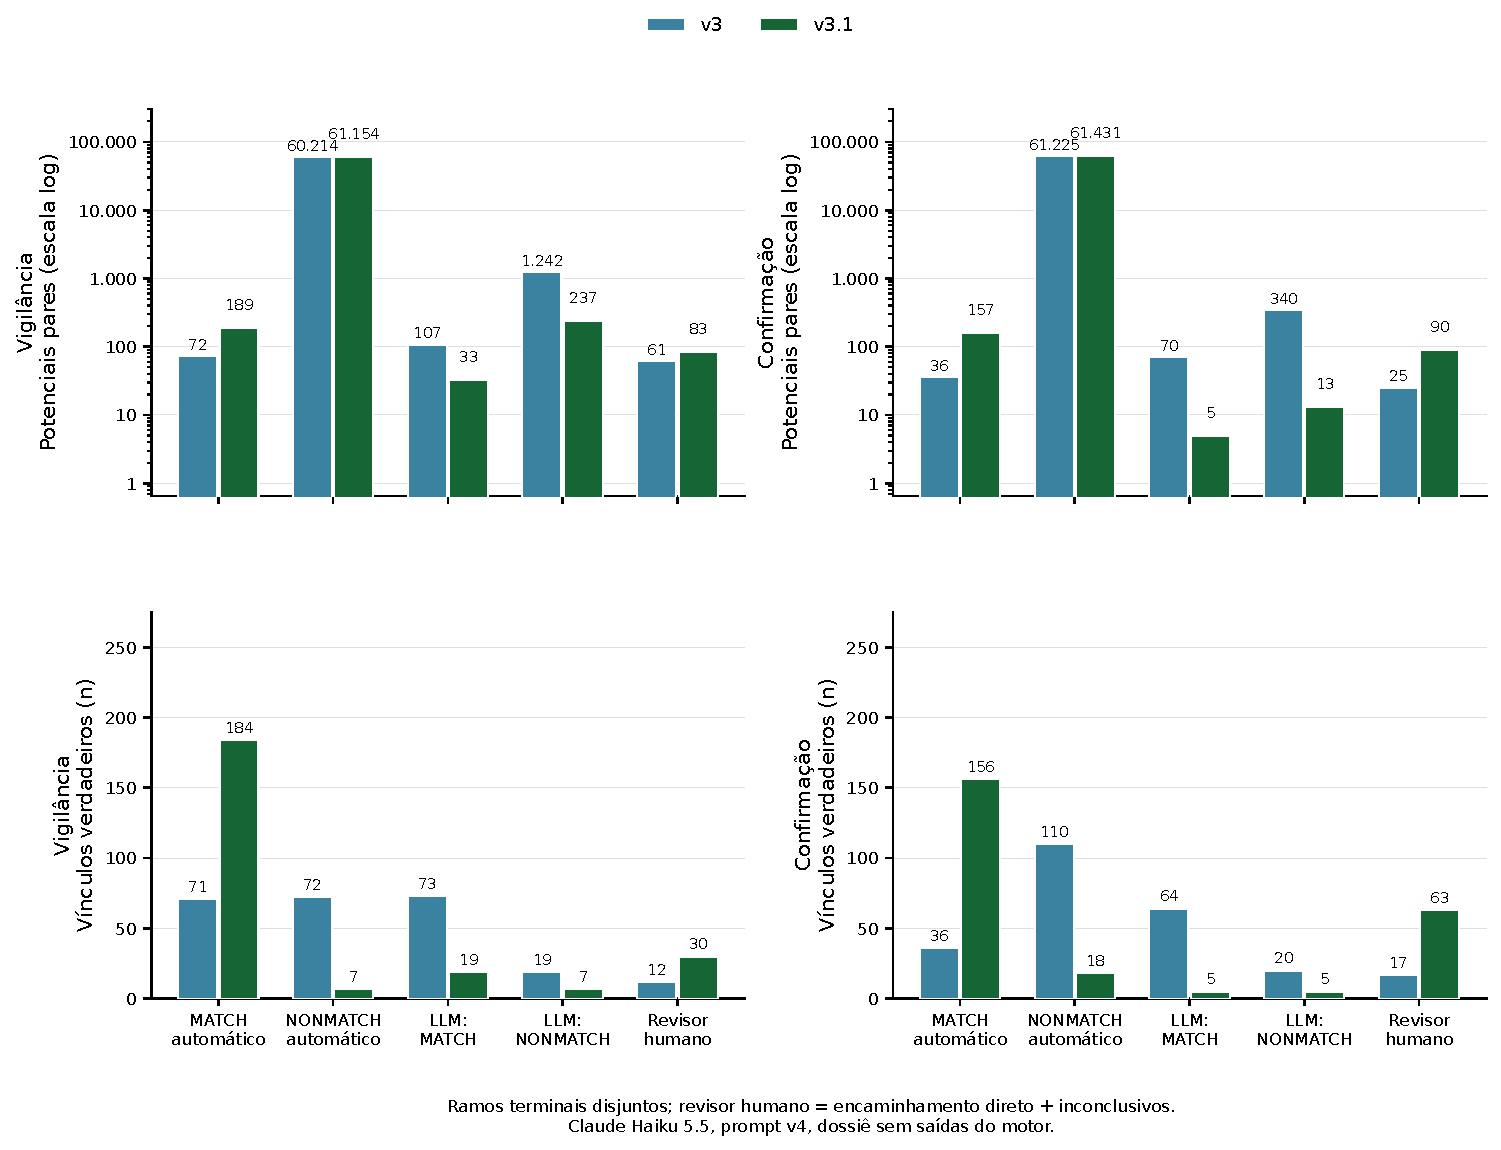
\includegraphics[width=\textwidth,height=0.75\textheight,keepaspectratio]{figures/fig_cap8_cascata_v31.pdf}
\caption{Cascata sobre a base inteira (comparação), com políticas v3 (três ações: vínculo, não vínculo e revisão LLM) e v3.1 (quatro ações, com revisão humana distinta da revisão LLM) nos modos vigilância e confirmação e Claude Haiku 5.5 com instruções v4 (versão sem solicitação das saídas do motor) e sem as saídas do motor. LLM designa modelo de linguagem de grande porte. Os ramos apresentam contagens de potenciais pares e vínculos segundo a referência operacional. Fonte: \texttt{data/funil\_gzcmd\_final.csv} e agregados correspondentes \cite{Jardim2026phdrepo}.}
\label{fig:cap8-cascata-v31}
\end{figure}

\subsection{Arranjo sequencial: resultado principal}\label{sec:e4-arranjo}

A Tabela~\ref{tab:cap8-referencia} situa a decisão principal frente à referência operacional e às comparações. A Tabela~\ref{tab:cap8-arranjo-corte} detalha os braços com registro interno anterior à S3 e o braço \textit{a posteriori}, exploratório, \textit{post hoc} e não registrado. Nos braços restritos, os 211 vínculos acima do corte são aceitos por construção e constituem o mínimo de aceitações desses braços. Os FP acima dele são zero pela definição de PAR, sem validação independente desse resultado.\footnote{S3 é a avaliação com os \textit{labels}.}

% Gerada por scripts/tabelas_arranjo_editorial.py; não editar manualmente.
\begin{table}[!ht]
\centering\footnotesize
\caption{Referência operacional, arranjo sequencial (resultado principal), cascatas sobre a base inteira (comparação) e cenários do Comparador de Registros (CdR), nos 61.696 potenciais pares e 247 vínculos. PAR~=~1 é definido pelo próprio corte do OpenRecLink (viés de verificação).}
\label{tab:cap8-referencia}
\resizebox{\linewidth}{!}{%
\begin{tabular}{llrrrrrr}
\toprule
Estratégia & Modo & Pares ao humano & Pares ao LLM & Sens. automática (\%) & FP automáticos & Vínculos perdidos & Sens. com humano (\%) \\
\midrule
\multicolumn{8}{l}{\textit{Referência operacional}} \\
OpenRecLink, corte isolado & ambos & 0 & 0 & 85,4 & 0 & 36 & n.a. \\
Corte + revisão clerical de origem & ambos & cenário $\geq 2.156$ & 0 & 85,4 & 0 & 0 & 100,0 \\
Corte + revisão humana integral (cenário) & ambos & 61.485 (teto) & 0 & 85,4 & 0 & 0 & 99,3 \\
\midrule
\multicolumn{8}{l}{\textit{Resultado principal}} \\
Arranjo sequencial P & vigilância & 96 & 344 & 87,0 & 21 & 13 & 94,4 \\
Arranjo sequencial P & confirmação & 17 & 41 & 88,7 & 4 & 27 & 89,0 \\
\midrule
\multicolumn{8}{l}{\textit{Comparação sobre a base inteira}} \\
Cascata v3.1 & vigilância & 111 & 347 & 78,5 & 34 & 15 & 93,2 \\
Cascata v3.1 & confirmação & 127 & 44 & 53,4 & 0 & 28 & 86,9 \\
Cascata v3 & vigilância & 61 & 1.410 & 58,3 & 35 & 91 & 62,9 \\
Cascata v3 & confirmação & 25 & 435 & 40,5 & 6 & 130 & 47,0 \\
\midrule
\multicolumn{8}{l}{\textit{Cenários hipotéticos do CdR}} \\
CdR, corte da nota em 9 & ambos & 0 & 0 & 37,7 & 2 & 154 & n.a. \\
CdR, decisão de limiar (nota $\geq 8$) & ambos & 0 & 0 & 51,4 & 70 & 120 & n.a. \\
CdR, revisão humana da área cinza da nota & ambos & 21.620 & 0 & 37,7 & 2 & 3 & 95,7 \\
\bottomrule
\end{tabular}}
\par\smallskip
\parbox{\linewidth}{\footnotesize (a) O corte aceita 211 vínculos; a revisão manual acrescenta 36. O volume examinado total e a ordem de revisão não foram registrados. Se a revisão tivesse seguido ordem decrescente do escore do OpenRecLink, o cenário exigiria pelo menos 2.156 potenciais pares, com limiar por passo, ou 2.522 com limiar global. A reconstrução é exploratória, \textit{post hoc} e não registrada, não carga histórica observada. (b) Os 100,0\% da linha corte + revisão manual decorrem da definição de PAR, não de acurácia observada. Zero FP acima do corte também decorre do \textit{label}. Em $[5,9)$ há 151 vínculos: 123 pelo corte e 28 pela revisão. Nessa faixa, o arranjo aceita 127 vínculos na vigilância e 127 na confirmação, incluindo 123 pelo corte em cada modo; a cascata sobre a base inteira aceita 113 e 65. (c) A revisão integral abaixo do corte é cenário de revisão de todos os 61.485 candidatos, não carga histórica medida. Sua sensibilidade é $(211+0{,}95\times36)/247$. (d) O arranjo corresponde ao braço P do registro interno versionado antes da avaliação com os \textit{labels} (S3), com emendas e suplemento. Seus FP estão abaixo do corte. Vínculos perdidos são apenas os classificados como não-vínculo, excluindo encaminhamentos pendentes. (e) A revisão da área cinza da nota do CdR é cenário com aceitação de notas $\geq9$ e descarte de notas $<5$, com sensibilidade $(93+0{,}95\times151)/247$. As células com humano, salvo a revisão clerical de origem incorporada ao \textit{label}, exibem o cenário de sensibilidade humana 0,95, não medida. Os três cenários, 0,95, 0,99 e 1,00, estão na Tabela~\ref{tab:cap8-sensibilidade-humana} e em \path{data/cenarios_sensibilidade_humana.csv}; a especificidade humana é perfeita por hipótese. O limiar 8 da nota é referência histórica do Estudo~3, não limiar escolhido para P. n.a.: não se aplica. Fontes: \path{data/carga_abaixo_corte.csv}, \path{data/referencia_comparador_pos_orl.csv}, \path{data/arranjo_corte_metricas.csv} e \path{data/funil_gzcmd_final_metricas.csv} \cite{Jardim2026phdrepo}.
}
\par\footnotesize P: arranjo principal, que preserva o corte do OpenRecLink e aplica a política com recalibração isotônica abaixo dele. PAR~=~2: vínculos recuperados na revisão clerical abaixo do corte. CdR: Comparador de Registros. Área cinza da nota: nota do CdR em $[5,9)$.
\end{table}


Na vigilância, o arranjo aceitou 215 dos 247 vínculos, 211 pelo corte e quatro pela política abaixo dele (87,0\%), frente aos 211 do corte isolado (85,4\%), proporção definida pela referência operacional. Os quatro vínculos adicionais acompanharam 21 FP e 13 vínculos perdidos por não-vínculo. Foram encaminhados 96 potenciais pares ao humano, incluindo 19 vínculos, e 344 ao LLM, com custo estimado de US\$~0,94. O fechamento é $215+13+19=247$. No cenário de sensibilidade humana $s=0{,}95$, a sensibilidade seria de 94,4\%, contra 99,3\% na revisão integral abaixo do corte; os cenários $s=0{,}99$ e $s=1{,}00$ constam da Tabela~\ref{tab:cap8-sensibilidade-humana}. O cenário hipotético de carga é apresentado na Seção~\ref{sec:padrao-ouro}. Todas as 25 aceitações abaixo do corte, quatro vínculos e 21 não vínculos, vieram do LLM. Nenhuma resultou das guardas ou da comparação automática de custos, conforme \path{data/arranjo_corte_s1_resumo.csv} e \path{data/arranjo_corte_metricas.csv}.

Na confirmação, o arranjo aceitou 219 vínculos, 211 pelo corte e oito pela política abaixo dele (88,7\%), com quatro FP e 27 vínculos perdidos. Foram 17 encaminhamentos humanos, incluindo um vínculo, e 41 ao LLM, a US\$~0,11. O fechamento é $219+27+1=247$, com sensibilidade projetada de 89,0\% após revisão humana no cenário $s=0{,}95$; os cenários $s=0{,}99$ e $s=1{,}00$ constam da Tabela~\ref{tab:cap8-sensibilidade-humana}. As 12 aceitações abaixo do corte, oito vínculos e quatro não vínculos, também vieram do LLM. As perdas foram de um vínculo pela guarda de nota $<5$, 22 por \texttt{AUTO\_NONMATCH} na comparação de custos e quatro por \texttt{NONMATCH} do LLM. Na vigilância, os respectivos mecanismos perderam um, seis e seis vínculos (\path{data/arranjo_corte_perdas_mecanismo.csv}). As 22 rejeições por custo ocorreram sob o perfil $C_{FP}=5C_{FN}$ da confirmação e sob a hipótese não medida $e_{FP,h}=0{,}05$: com $C_{FP}=100$, $\mathcal{L}_H(p)=6-4p$ e a revisão humana só supera o não vínculo para $p>0{,}25$, contra $p>0{,}05$ sem erro humano (cálculo da tese). Na base inteira, com $C_{LLM}=0{,}005$, essa hipótese reduz os encaminhamentos diretos de 229 para 121 e a sensibilidade esperada com humano de 92,3\% para 87,7\% (\path{data/varredura_custos_confirmacao.csv}), embora a avaliação trate a especificidade humana como perfeita. A varredura da Seção~\ref{sec:e4-varredura-custos} refere-se à base inteira; no arranjo não houve varredura de custos. A decomposição não isola o efeito causal da razão de custos em relação à calibração.

% Gerada por scripts/tabelas_arranjo_editorial.py; não editar manualmente.
\begingroup
\scriptsize
\setlength{\tabcolsep}{2pt}
\begin{longtable}{lrrrrrrrrr}
\caption[Arranjo sequencial: decisões, revisão e custo]{Arranjo sequencial OpenRecLink e GZ-CMD v3.1, Claude Haiku 5.5, instruções v4: decisões, revisão e custo. São 247 pares verdadeiros na base e 151 em $[5,9)$. PAR~=~1 é definido pelo corte; as classes PAR~=~1 e PAR~=~2 não comprovam incorporação, que depende das evidências usadas na referência. Predição fora da amostra não equivale a validação externa.}
\label{tab:cap8-arranjo-corte}\\
\toprule
Braço & $V_A$ & $S_A$ (\%) & FP automáticos (abaixo) & $V_N$ & $H$ ($V_H$) & LLM & Chamadas & US\$ & $S_H$ (5\%) \\
\midrule
\endfirsthead
\toprule
Braço & $V_A$ & $S_A$ (\%) & FP automáticos (abaixo) & $V_N$ & $H$ ($V_H$) & LLM & Chamadas & US\$ & $S_H$ (5\%) \\
\midrule
\endhead
\bottomrule
\endlastfoot
\multicolumn{10}{l}{\textbf{Vigilância: base inteira}} \\
(i) Corte & 211 & 85,4 & 0 (0) & 36 & 0 (0) & 0 & 0 & 0,0000 & 85,4 \\
Cascata sobre a base inteira & 194 & 78,5 & 34 (34) & 15 & 111 (38) & 347 & 747 & 0,9198 & 93,2 \\
B1 & 194 & 78,5 & 40 (40) & 15 & 115 (38) & 374 & 821 & 1,0178 & 93,2 \\
(ii) Humano integral & 211 & 85,4 & 0 (0) & 0 & 61.485 (teto; 36) & 0 & 0 & 0,0000 & 99,3 \\
\textit{A posteriori} (sem registro interno) & 221 & 89,5 & 34 (34) & 9 & 90 (17) & 330 & 710 & 0,8750 & 96,0 \\
ASR & 215 & 87,0 & 21 (21) & 13 & 96 (19) & 344 & 755 & 0,9380 & 94,4 \\
ASR-Platt & 217 & 87,9 & 3 (3) & 13 & 77 (17) & 110 & 239 & 0,3013 & 94,4 \\
A3 & 219 & 88,7 & 19 (19) & 14 & 100 (14) & 367 & 806 & 1,0107 & 94,0 \\
ASR-PAR2-faixa & 211 & 85,4 & 21 (21) & 12 & 116 (24) & 265 & 583 & 0,7252 & 94,7 \\
\midrule
\multicolumn{10}{l}{\textbf{Vigilância: faixa intermediária da nota final $[5,9)$}} \\
(i) Corte & 123 & 81,5 & 0 (0) & 28 & 0 (0) & 0 & 0 & 0,0000 & 81,5 \\
Cascata sobre a base inteira & 113 & 74,8 & 34 (34) & 12 & 97 (26) & 347 & 747 & 0,9198 & 91,2 \\
B1 & 113 & 74,8 & 40 (40) & 12 & 101 (26) & 374 & 821 & 1,0178 & 91,2 \\
(ii) Humano integral & 123 & 81,5 & 0 (0) & 0 & 21.497 (teto; 28) & 0 & 0 & 0,0000 & 99,1 \\
\textit{A posteriori} (sem registro interno) & 131 & 86,8 & 34 (34) & 8 & 83 (12) & 330 & 710 & 0,8750 & 94,3 \\
ASR & 127 & 84,1 & 21 (21) & 11 & 89 (13) & 342 & 751 & 0,9327 & 92,3 \\
ASR-Platt & 127 & 84,1 & 3 (3) & 12 & 71 (12) & 107 & 232 & 0,2928 & 91,7 \\
A3 & 129 & 85,4 & 19 (19) & 11 & 96 (11) & 362 & 796 & 0,9989 & 92,4 \\
ASR-PAR2-faixa & 123 & 81,5 & 21 (21) & 10 & 109 (18) & 263 & 579 & 0,7199 & 92,8 \\
\midrule
\multicolumn{10}{l}{\textbf{Confirmação: base inteira}} \\
(i) Corte & 211 & 85,4 & 0 (0) & 36 & 0 (0) & 0 & 0 & 0,0000 & 85,4 \\
Cascata sobre a base inteira & 132 & 53,4 & 0 (0) & 28 & 127 (87) & 44 & 95 & 0,1192 & 86,9 \\
B1 & 131 & 53,0 & 4 (4) & 30 & 131 (86) & 70 & 151 & 0,1848 & 86,1 \\
(ii) Humano integral & 211 & 85,4 & 0 (0) & 0 & 61.485 (teto; 36) & 0 & 0 & 0,0000 & 99,3 \\
\textit{A posteriori} (sem registro interno) & 219 & 88,7 & 0 (0) & 17 & 51 (11) & 25 & 53 & 0,0656 & 92,9 \\
ASR & 219 & 88,7 & 4 (4) & 27 & 17 (1) & 41 & 87 & 0,1052 & 89,0 \\
ASR-Platt & 219 & 88,7 & 3 (3) & 27 & 16 (1) & 25 & 54 & 0,0654 & 89,0 \\
A3 & 219 & 88,7 & 5 (5) & 23 & 22 (5) & 32 & 67 & 0,0783 & 90,6 \\
ASR-PAR2-faixa & 217 & 87,9 & 0 (0) & 26 & 22 (4) & 18 & 37 & 0,0441 & 89,4 \\
\midrule
\multicolumn{10}{l}{\textbf{Confirmação: faixa intermediária da nota final $[5,9)$}} \\
(i) Corte & 123 & 81,5 & 0 (0) & 28 & 0 (0) & 0 & 0 & 0,0000 & 81,5 \\
Cascata sobre a base inteira & 65 & 43,0 & 0 (0) & 20 & 106 (66) & 30 & 64 & 0,0793 & 84,6 \\
B1 & 64 & 42,4 & 4 (4) & 22 & 110 (65) & 56 & 120 & 0,1449 & 83,3 \\
(ii) Humano integral & 123 & 81,5 & 0 (0) & 0 & 21.497 (teto; 28) & 0 & 0 & 0,0000 & 99,1 \\
\textit{A posteriori} (sem registro interno) & 127 & 84,1 & 0 (0) & 13 & 51 (11) & 18 & 38 & 0,0471 & 91,0 \\
ASR & 127 & 84,1 & 4 (4) & 23 & 17 (1) & 32 & 68 & 0,0821 & 84,7 \\
ASR-Platt & 127 & 84,1 & 3 (3) & 23 & 16 (1) & 16 & 35 & 0,0423 & 84,7 \\
A3 & 127 & 84,1 & 5 (5) & 19 & 22 (5) & 26 & 54 & 0,0626 & 87,3 \\
ASR-PAR2-faixa & 125 & 82,8 & 0 (0) & 22 & 22 (4) & 9 & 18 & 0,0209 & 85,3 \\
\end{longtable}
\par\footnotesize ASR: arranjo sequencial do registro interno, que preserva o corte do OpenRecLink e aplica a política com recalibração isotônica abaixo dele. PAR~=~2: pares verdadeiros recuperados na revisão manual de origem abaixo do corte. B1: mantém a base inteira e a probabilidade original, substituindo apenas as proporções de erro do revisor. A3: restringe também o treinamento do classificador à região abaixo do corte. ASR-PAR2-faixa: estima a omissão do revisor somente nos pares verdadeiros PAR~=~2 e agrupa as faixas da nota final em $[5,9)$. ASR-Platt: análise de sensibilidade de ASR com \textit{Platt scaling} abaixo do corte. Braço \textit{a posteriori}: cascata sobre a base inteira aplicada abaixo do corte, sem recalibração. Viés de incorporação: uso, na construção da referência, das mesmas evidências avaliadas pelo método.

\noindent\parbox{\linewidth}{\footnotesize $V_A$: pares verdadeiros aceitos automaticamente, inclusive \texttt{MATCH} do modelo de linguagem (LLM); $V_N$: pares verdadeiros perdidos por \texttt{NONMATCH}; $H$: potenciais pares ao revisor humano, com pares verdadeiros $V_H$ entre parênteses. UNSURE do LLM segue ao humano uma única vez. LLM e humano se sobrepõem nesse encaminhamento, sem somar novamente sua carga humana. $S_A=V_A/n$; $S_H=(V_A+0{,}95V_H)/n$ exibe o cenário de sensibilidade humana 0,95, não resultado humano observado. Os três cenários, 0,95, 0,99 e 1,00, constam da Tabela~\ref{tab:cap8-sensibilidade-humana} e de \path{data/cenarios_sensibilidade_humana.csv}; a especificidade humana é perfeita por hipótese. Custos usam somente os registros de consumo dos potenciais pares selecionados por cada braço e faixa, com tarifas históricas por tokens, não faturas. O braço \textit{a posteriori} preserva o corte e aplica a cascata sobre a base inteira abaixo dele, sem recalibração. Fonte: \texttt{data/arranjo\_corte\_metricas.csv} e \texttt{data/arranjo\_corte\_par2.csv}.}
\begin{longtable}{lrrr}
\caption{Partição dos 36 pares verdadeiros PAR~=~2 abaixo do corte. Cada célula mostra a contagem e seu IC de Wilson de 95\%, em porcentagem. As ressalvas sobre a referência operacional e a dependência entre pares permanecem.}
\label{tab:cap8-arranjo-corte-par2}\\
\toprule
Braço & Aceitos (IC 95\%) & Humano (IC 95\%) & Perdidos (IC 95\%) \\
\midrule
\multicolumn{4}{l}{\textbf{Vigilância}} \\
(i) Corte & 0 [0,0; 9,6] & 0 [0,0; 9,6] & 36 [90,4; 100,0] \\
Cascata sobre a base inteira & 10 [15,8; 44,0] & 17 [32,0; 63,0] & 9 [13,8; 41,1] \\
B1 & 8 [11,7; 38,1] & 19 [37,0; 68,0] & 9 [13,8; 41,1] \\
(ii) Humano integral & 0 [0,0; 9,6] & 36 [90,4; 100,0] & 0 [0,0; 9,6] \\
\textit{A posteriori} (sem registro interno) & 10 [15,8; 44,0] & 17 [32,0; 63,0] & 9 [13,8; 41,1] \\
ASR & 4 [4,4; 25,3] & 19 [37,0; 68,0] & 13 [22,5; 52,4] \\
ASR-Platt & 6 [7,9; 31,9] & 17 [32,0; 63,0] & 13 [22,5; 52,4] \\
A3 & 8 [11,7; 38,1] & 14 [24,8; 55,1] & 14 [24,8; 55,1] \\
ASR-PAR2-faixa & 0 [0,0; 9,6] & 24 [50,3; 79,8] & 12 [20,2; 49,7] \\
\midrule
\multicolumn{4}{l}{\textbf{Confirmação}} \\
(i) Corte & 0 [0,0; 9,6] & 0 [0,0; 9,6] & 36 [90,4; 100,0] \\
Cascata sobre a base inteira & 8 [11,7; 38,1] & 11 [18,0; 46,9] & 17 [32,0; 63,0] \\
B1 & 8 [11,7; 38,1] & 11 [18,0; 46,9] & 17 [32,0; 63,0] \\
(ii) Humano integral & 0 [0,0; 9,6] & 36 [90,4; 100,0] & 0 [0,0; 9,6] \\
\textit{A posteriori} (sem registro interno) & 8 [11,7; 38,1] & 11 [18,0; 46,9] & 17 [32,0; 63,0] \\
ASR & 8 [11,7; 38,1] & 1 [0,5; 14,2] & 27 [58,9; 86,2] \\
ASR-Platt & 8 [11,7; 38,1] & 1 [0,5; 14,2] & 27 [58,9; 86,2] \\
A3 & 8 [11,7; 38,1] & 5 [6,1; 28,7] & 23 [47,6; 77,5] \\
ASR-PAR2-faixa & 6 [7,9; 31,9] & 4 [4,4; 25,3] & 26 [56,0; 84,2] \\
\bottomrule
\end{longtable}
\par\footnotesize ASR: arranjo sequencial do registro interno, que preserva o corte do OpenRecLink e aplica a política com recalibração isotônica abaixo dele. PAR~=~2: pares verdadeiros recuperados na revisão manual de origem abaixo do corte. B1: mantém a base inteira e a probabilidade original, substituindo apenas as proporções de erro do revisor. A3: restringe também o treinamento do classificador à região abaixo do corte. ASR-PAR2-faixa: estima a omissão do revisor somente nos pares verdadeiros PAR~=~2 e agrupa as faixas da nota final em $[5,9)$. ASR-Platt: análise de sensibilidade de ASR com \textit{Platt scaling} abaixo do corte. Braço \textit{a posteriori}: cascata sobre a base inteira aplicada abaixo do corte, sem recalibração. Viés de incorporação: uso, na construção da referência, das mesmas evidências avaliadas pelo método.

\endgroup


Entre os 36 vínculos PAR~=~2 (Tabela~\ref{tab:cap8-arranjo-corte-par2}), a vigilância aceitou quatro (11,1\%; IC 95\%: 4,4 a 25,3), encaminhou 19 ao humano (52,8\%; 37,0 a 68,0) e perdeu 13 (36,1\%; 22,5 a 52,4). Na confirmação, foram oito aceitos (22,2\%; 11,7 a 38,1), um ao humano (2,8\%; 0,5 a 14,2) e 27 perdidos (75,0\%; 58,9 a 86,2). Essas perdas medem o que o arranjo deixa de recuperar frente aos vínculos documentados no processo de \textit{linkage} de origem, em troca de 96 e 17 encaminhamentos humanos. As aceitações são aninhadas: P acrescenta exatamente quatro e oito vínculos ao corte; sobreposição de intervalos marginais não é teste dessa diferença.\footnote{P é o arranjo principal com calibração isotônica abaixo do corte.}

Na área cinza da nota, que contém 151 vínculos, o corte aceita 123. O arranjo aceitou 127 nos dois modos (84,1\%), incluindo quatro PAR~=~2. Na vigilância, foram 21 FP, 89 encaminhamentos humanos e 342 ao LLM; na confirmação, quatro FP, 17 ao humano e 32 ao LLM. A cascata sobre a base inteira aceitou 113 e 65 vínculos nessa faixa, abaixo dos 123 aceitos pelo corte. O acréscimo automático frente ao corte isolado é pequeno e não elimina a perda de 13 e 27 dos 36 vínculos PAR~=~2, no conjunto abaixo do corte.

Frente à cascata sobre a base inteira, o arranjo passou de 194 para 215 vínculos aceitos na vigilância, de 34 para 21 FP e de 111 para 96 encaminhamentos humanos. Na confirmação, passou de 132 para 219 aceitos, de zero para quatro FP e de 127 para 17 encaminhamentos. Os lotes LLM foram próximos: 344 contra 347 e 41 contra 44. A vantagem na aceitação total vem inteiramente dos 211 vínculos PAR~=~1 preservados por construção: a cascata sobre a base inteira não aceitou automaticamente 27 e 87 deles (\path{data/sensibilidade_gzcmd_por_par.csv}). Nos 36 vínculos PAR~=~2, o arranjo aceitou quatro contra dez na vigilância, encaminhou 19 contra 17 ao humano e perdeu 13 contra nove. Na confirmação, aceitou oito contra oito, encaminhou um contra 11 e perdeu 27 contra 17 (\path{data/arranjo_corte_par2.csv}). A ponte B1 aceitou 194 e 131, com 40 e quatro FP. O braço \textit{a posteriori} aceitou 221 e 219, com 34 e zero FP e 90 e 51 encaminhamentos humanos; na vigilância, aceitou mais, perdeu menos (nove contra 13) e encaminhou menos que P, mas teve mais FP; na confirmação, teve menos FP e perdas que P, ao custo de mais encaminhamentos. É exploratório, \textit{post hoc} e não registrado e não substitui P.\footnote{B1 é a ponte que mantém a probabilidade original e troca apenas as proporções do revisor.}

P foi dominado por P-Platt na avaliação original. P-Platt aceitou 217 vínculos na vigilância, com três FP, 77 encaminhamentos humanos e 110 ao LLM, a US\$~0,30; na confirmação, foram 219 aceitos, três FP, 16 ao humano e 25 ao LLM. Na vigilância, reduziu FP, encaminhamentos e custo frente a P, mantendo os mesmos 13 vínculos perdidos. A3 aceitou 219 nos dois modos, com 19 e cinco FP; P-PAR2-grey aceitou 211 e 217, com 21 e zero FP. A ponte B1 mostra que substituir apenas as proporções do revisor também altera decisões: não se deve atribuir toda diferença da cadeia à recalibração abaixo do corte. P permanece o resultado principal do registro interno. A dominância original não foi sustentada na análise de estabilidade descrita abaixo \cite{Jardim2026phdrepo}.\footnote{P-Platt é a análise de sensibilidade de P com \textit{Platt scaling} abaixo do corte.}

Cada braço soma apenas o consumo registrado dos potenciais pares selecionados, com tarifas históricas, sem representar fatura do provedor. As 24 respostas novas e as 69 do suplemento tiveram custo estimado conjunto de US\$~0,2448, soma de US\$~0,063 das respostas novas e US\$~0,1819 do suplemento, sem realimentar as proporções congeladas do revisor (\path{data/arranjo_corte_metadata.json}, campo \texttt{cost\_sources}, e \path{data/sprint3b/anthropic_sem_mo_v4_arranjo_corte_supl/execucao.json}).

\subsection{Estabilidade não confirmatória do arranjo}\label{sec:e4-robustez}

A dominância de P-Platt sobre P não foi sustentada nos dois modos (Tabela~\ref{tab:cap8-robustez-arranjo}): ocorreu em 7/20 réplicas do bloco numérico e 4/20 do bloco de partição na vigilância, e em 7/20 e 5/20 na confirmação. A dominância inversa foi 0/20 em todos os blocos. Na vigilância, a vantagem de P-Platt em FP foi estável: P menos P-Platt foi positivo em 20/20 nos dois blocos. Essa vantagem teve compensações. A mediana da diferença P menos P-Platt foi de $-1$ vínculo perdido no bloco numérico e $-2$ no bloco de partição, com mais 16,5 e 17 potenciais pares ao humano e mais 221 e 170,5 ao LLM, respectivamente. P-Platt perdeu, portanto, um a dois vínculos a mais em mediana, encaminhando menos pares para revisão (\path{data/robustez_arranjo_resumo.csv}).\footnote{P é o arranjo principal com calibração isotônica abaixo do corte; P-Platt é a análise de sensibilidade de P com \textit{Platt scaling} abaixo do corte.}

\begin{table}[!ht]
\centering
\caption{Estabilidade da dominância de P-Platt (análise de sensibilidade de P com \textit{Platt scaling} abaixo do corte) sobre P (arranjo principal com calibração isotônica abaixo do corte) entre réplicas, isto é, reexecuções com outra semente, número de processos paralelos ou partição.}
\label{tab:cap8-robustez-arranjo}
\begin{minipage}{\linewidth}
\centering
% Gerada por scripts/arranjo_robustez.py, fase C.
\begin{tabular}{lrrrl}
\toprule
Modo & Numérico & Partição & Inversa (num.; part.) & Classificação \\
\midrule
Vigilância & 7/20 & 4/20 & 0/20; 0/20 & não sustentada \\
Confirmação & 7/20 & 5/20 & 0/20; 0/20 & não sustentada \\
\bottomrule
\end{tabular}
\par\noindent\footnotesize Análise não confirmatória. P permanece o braço principal. Dominância fraca de P-Platt sobre P, com ao menos uma desigualdade estrita, nos vínculos aceitos, falsos positivos abaixo do corte, vínculos perdidos e potenciais pares ao revisor humano e ao modelo de linguagem. Os modos são avaliados separadamente. Fonte: \texttt{data/robustez\_arranjo\_resumo.csv}.
\par\footnotesize P: arranjo principal, que preserva o corte do OpenRecLink e aplica a política com recalibração isotônica abaixo dele. P-Platt: análise de sensibilidade de P com \textit{Platt scaling} abaixo do corte. Numérico e Partição: réplicas com dominância de P-Platt sobre P, em 20 reexecuções de cada bloco. Inversa: réplicas com dominância de P sobre P-Platt nos blocos numérico e de partição, respectivamente.

\end{minipage}
\end{table}

Na vigilância, as perdas de PAR~=~2 de P tiveram mediana 13, com mínimo 10 e máximo 16 no bloco numérico; no bloco de partição, mediana 14, mínimo 9 e máximo 21. P perdeu mais PAR~=~2 que o braço \textit{a posteriori} em 20/20 e 19/20 réplicas desses blocos; na confirmação, em 20/20 de ambos. O Jaccard do lote de encaminhamento ao revisor LLM em relação à partição original teve mediana 0,427 em P na vigilância no bloco de partição e 0,726 no bloco numérico. A variação de \textit{threads} e semente do classificador alterou a probabilidade de P em até 0,65 no bloco numérico; com outras partições, a diferença máxima chegou a 0,80 (\path{data/robustez_arranjo_resumo.csv}). No bloco de partição da vigilância, os FP de P variaram de 9 a 31. A réplica original é um ponto dessa distribuição, não seu resultado típico garantido. A instabilidade da seleção impede interpretar a avaliação pontual como escolha estável dos pares a revisar.

Os contadores de dominância não ponderam os desfechos. Aplicando os custos declarados de cada modo ($C_{FP}=10$ e $C_{FN}=50$ na vigilância; $C_{FP}=100$ e $C_{FN}=20$ na confirmação; $C_H=1$ e $C_{LLM}=0{,}005$ nos dois) às medianas de FP, perdidos e encaminhamentos, P-Platt tem perda menor que P nos quatro cenários: a diferença P menos P-Platt é de 144,1 e 94,4 nos blocos numérico e de partição da vigilância e de 101,6 e 143,0 na confirmação. A soma ponderada das medianas das diferenças pareadas dá 147,6, 47,9, 102,1 e 103,5, na mesma ordem (\path{data/robustez_perda_ponderada.csv}). São perdas aplicadas às medianas marginais, não a mediana da perda por réplica. A calibração isotônica de P também variou mais entre réplicas: no bloco numérico, a mediana da maior diferença de probabilidade em relação à réplica original foi de 0,46 em P, com máximo de 0,65, contra 0,17 em P-Platt, com máximo de 0,22; o Jaccard mediano do lote LLM na vigilância foi de 0,726 em P e de 0,819 em P-Platt. A isotônica em P é decisão do registro \texttt{8c16a41}, não resultado de comparação: na primeira partição externa, o conjunto de calibração tinha 32 vínculos PAR~=~2 entre 49.189 potenciais pares (\path{gzcmd/prereg_arranjo_corte.yaml}, diagnóstico da emenda 1). A estabilidade, portanto, não sustenta superioridade de P.

As 242 revisões novas da análise de estabilidade tiveram custo estimado de US\$~0,6255. Somadas aos US\$~0,2448 do arranjo inicial, totalizam US\$~0,8703 (\path{data/robustez_arranjo_metadata.json} e \path{data/arranjo_corte_metadata.json}). Com os US\$~0,2633 das chamadas do filtro LLM (\path{data/filtro_llm_metadata.json}), as execuções novas somam US\$~1,13 ($0{,}2448+0{,}6255+0{,}2633=1{,}1336$), sem incluir pessoal e infraestrutura nem os cerca de US\$~76 da avaliação do Claude Sonnet 5.5 (Seção~\ref{sec:e4-reruns}), que não integra o arranjo.

\subsection{Ordenação na mesma carga e curva de esforço}\label{sec:e4-mesma-carga}

As comparações desta seção são exploratórias, \textit{post hoc} e não registradas, salvo indicação do protocolo do filtro adiante. O1 ordena pelo escore do OpenRecLink; O2, pela nota do CdR; O3, pela probabilidade calibrada do classificador na base inteira; O4, pela probabilidade recalibrada de P. O3 e O4 utilizam o mesmo XGBoost avaliado fora da amostra e os mesmos \textit{labels} verificados. A Figura~\ref{fig:cap8-curva-esforco} e a Tabela~\ref{tab:cap8-mesma-carga} relacionam o orçamento à recuperação, sem presumir a ordem histórica de revisão. A recuperação dos encaminhamentos de P e das ordenações pressupõe revisor perfeito nos dois lados; não corresponde a acerto humano observado.\footnote{P é o arranjo principal com calibração isotônica abaixo do corte; CdR designa o Comparador de Registros.}

\begin{figure}[!htbp]
\centering
\resizebox{\linewidth}{!}{% Gerado por scripts/figura_curva_esforco.py; não editar.
\begin{pgfpicture}
\pgfsetlinewidth{0.35pt}
\pgfpathrectangle{\pgfpoint{0cm}{0cm}}{\pgfpoint{11.4cm}{3.1cm}}\pgfusepath{stroke}
\pgftext[right,at={\pgfpoint{-0.18000cm}{0.00000cm}}]{\scriptsize 0}
\pgftext[right,at={\pgfpoint{-0.18000cm}{0.77500cm}}]{\scriptsize 9}
\pgftext[right,at={\pgfpoint{-0.18000cm}{1.55000cm}}]{\scriptsize 18}
\pgftext[right,at={\pgfpoint{-0.18000cm}{2.32500cm}}]{\scriptsize 27}
\pgftext[right,at={\pgfpoint{-0.18000cm}{3.10000cm}}]{\scriptsize 36}
\pgftext[at={\pgfpoint{0.00000cm}{-0.23000cm}}]{\scriptsize 1}
\pgftext[at={\pgfpoint{3.35122cm}{-0.23000cm}}]{\scriptsize 10}
\pgftext[at={\pgfpoint{6.70244cm}{-0.23000cm}}]{\scriptsize 100}
\pgftext[at={\pgfpoint{10.05366cm}{-0.23000cm}}]{\scriptsize 1.000}
\pgftext[at={\pgfpoint{11.40000cm}{-0.23000cm}}]{\scriptsize 2.522}
\pgftext[at={\pgfpoint{5.70000cm}{-0.60000cm}}]{\scriptsize Revisões humanas (escala logarítmica)}
\pgftext[left,at={\pgfpoint{0.00000cm}{3.37000cm}}]{\scriptsize PAR=2 recuperados, revisor perfeito}
\color{gray}
\pgfsetdash{}{0pt}
\pgfsetlinewidth{0.9pt}
\pgfpathmoveto{\pgfpoint{0.00000cm}{0.00000cm}}
\pgfpathlineto{\pgfpoint{1.00882cm}{0.00000cm}}
\pgfpathlineto{\pgfpoint{1.00882cm}{0.08611cm}}
\pgfpathlineto{\pgfpoint{2.01764cm}{0.08611cm}}
\pgfpathlineto{\pgfpoint{2.01764cm}{0.17222cm}}
\pgfpathlineto{\pgfpoint{3.84093cm}{0.17222cm}}
\pgfpathlineto{\pgfpoint{3.84093cm}{0.25833cm}}
\pgfpathlineto{\pgfpoint{4.90082cm}{0.25833cm}}
\pgfpathlineto{\pgfpoint{4.90082cm}{0.34444cm}}
\pgfpathlineto{\pgfpoint{5.33201cm}{0.34444cm}}
\pgfpathlineto{\pgfpoint{5.33201cm}{0.43056cm}}
\pgfpathlineto{\pgfpoint{5.36886cm}{0.43056cm}}
\pgfpathlineto{\pgfpoint{5.36886cm}{0.51667cm}}
\pgfpathlineto{\pgfpoint{5.47411cm}{0.51667cm}}
\pgfpathlineto{\pgfpoint{5.47411cm}{0.60278cm}}
\pgfpathlineto{\pgfpoint{5.57227cm}{0.60278cm}}
\pgfpathlineto{\pgfpoint{5.57227cm}{0.68889cm}}
\pgfpathlineto{\pgfpoint{5.72245cm}{0.68889cm}}
\pgfpathlineto{\pgfpoint{5.72245cm}{0.77500cm}}
\pgfpathlineto{\pgfpoint{5.75071cm}{0.77500cm}}
\pgfpathlineto{\pgfpoint{5.75071cm}{0.86111cm}}
\pgfpathlineto{\pgfpoint{5.80563cm}{0.86111cm}}
\pgfpathlineto{\pgfpoint{5.80563cm}{0.94722cm}}
\pgfpathlineto{\pgfpoint{5.88432cm}{0.94722cm}}
\pgfpathlineto{\pgfpoint{5.88432cm}{1.03333cm}}
\pgfpathlineto{\pgfpoint{6.02999cm}{1.03333cm}}
\pgfpathlineto{\pgfpoint{6.02999cm}{1.11944cm}}
\pgfpathlineto{\pgfpoint{6.05291cm}{1.11944cm}}
\pgfpathlineto{\pgfpoint{6.05291cm}{1.20556cm}}
\pgfpathlineto{\pgfpoint{6.07547cm}{1.20556cm}}
\pgfpathlineto{\pgfpoint{6.07547cm}{1.29167cm}}
\pgfpathlineto{\pgfpoint{6.09769cm}{1.29167cm}}
\pgfpathlineto{\pgfpoint{6.09769cm}{1.37778cm}}
\pgfpathlineto{\pgfpoint{6.11958cm}{1.37778cm}}
\pgfpathlineto{\pgfpoint{6.11958cm}{1.46389cm}}
\pgfpathlineto{\pgfpoint{6.14114cm}{1.46389cm}}
\pgfpathlineto{\pgfpoint{6.14114cm}{1.55000cm}}
\pgfpathlineto{\pgfpoint{6.22433cm}{1.55000cm}}
\pgfpathlineto{\pgfpoint{6.22433cm}{1.63611cm}}
\pgfpathlineto{\pgfpoint{7.65941cm}{1.63611cm}}
\pgfpathlineto{\pgfpoint{7.65941cm}{1.72222cm}}
\pgfpathlineto{\pgfpoint{8.55047cm}{1.72222cm}}
\pgfpathlineto{\pgfpoint{8.55047cm}{1.80833cm}}
\pgfpathlineto{\pgfpoint{8.99148cm}{1.80833cm}}
\pgfpathlineto{\pgfpoint{8.99148cm}{1.89444cm}}
\pgfpathlineto{\pgfpoint{9.04775cm}{1.89444cm}}
\pgfpathlineto{\pgfpoint{9.04775cm}{1.98056cm}}
\pgfpathlineto{\pgfpoint{9.33426cm}{1.98056cm}}
\pgfpathlineto{\pgfpoint{9.33426cm}{2.06667cm}}
\pgfpathlineto{\pgfpoint{9.39042cm}{2.06667cm}}
\pgfpathlineto{\pgfpoint{9.39042cm}{2.15278cm}}
\pgfpathlineto{\pgfpoint{10.04490cm}{2.15278cm}}
\pgfpathlineto{\pgfpoint{10.04490cm}{2.23889cm}}
\pgfpathlineto{\pgfpoint{10.04637cm}{2.23889cm}}
\pgfpathlineto{\pgfpoint{10.04637cm}{2.32500cm}}
\pgfpathlineto{\pgfpoint{10.04929cm}{2.32500cm}}
\pgfpathlineto{\pgfpoint{10.04929cm}{2.41111cm}}
\pgfpathlineto{\pgfpoint{10.13297cm}{2.41111cm}}
\pgfpathlineto{\pgfpoint{10.13297cm}{2.49722cm}}
\pgfpathlineto{\pgfpoint{10.13847cm}{2.49722cm}}
\pgfpathlineto{\pgfpoint{10.13847cm}{2.58333cm}}
\pgfpathlineto{\pgfpoint{10.26213cm}{2.58333cm}}
\pgfpathlineto{\pgfpoint{10.26213cm}{2.66944cm}}
\pgfpathlineto{\pgfpoint{11.38550cm}{2.66944cm}}
\pgfpathlineto{\pgfpoint{11.38550cm}{2.75556cm}}
\pgfpathlineto{\pgfpoint{11.38725cm}{2.75556cm}}
\pgfpathlineto{\pgfpoint{11.38725cm}{2.84167cm}}
\pgfpathlineto{\pgfpoint{11.39190cm}{2.84167cm}}
\pgfpathlineto{\pgfpoint{11.39190cm}{2.92778cm}}
\pgfpathlineto{\pgfpoint{11.39711cm}{2.92778cm}}
\pgfpathlineto{\pgfpoint{11.39711cm}{3.01389cm}}
\pgfpathlineto{\pgfpoint{11.39942cm}{3.01389cm}}
\pgfpathlineto{\pgfpoint{11.39942cm}{3.10000cm}}
\pgfpathlineto{\pgfpoint{11.40000cm}{3.10000cm}}
\pgfusepath{stroke}
\color{orange}
\pgfsetdash{{4pt}{2pt}}{0pt}
\pgfsetlinewidth{0.9pt}
\pgfpathmoveto{\pgfpoint{0.00000cm}{0.08611cm}}
\pgfpathlineto{\pgfpoint{1.00882cm}{0.08611cm}}
\pgfpathlineto{\pgfpoint{1.00882cm}{0.17222cm}}
\pgfpathlineto{\pgfpoint{1.59894cm}{0.17222cm}}
\pgfpathlineto{\pgfpoint{1.59894cm}{0.25833cm}}
\pgfpathlineto{\pgfpoint{2.01764cm}{0.25833cm}}
\pgfpathlineto{\pgfpoint{2.01764cm}{0.34444cm}}
\pgfpathlineto{\pgfpoint{2.60776cm}{0.34444cm}}
\pgfpathlineto{\pgfpoint{2.60776cm}{0.43056cm}}
\pgfpathlineto{\pgfpoint{3.02645cm}{0.43056cm}}
\pgfpathlineto{\pgfpoint{3.02645cm}{0.51667cm}}
\pgfpathlineto{\pgfpoint{3.19788cm}{0.51667cm}}
\pgfpathlineto{\pgfpoint{3.19788cm}{0.60278cm}}
\pgfpathlineto{\pgfpoint{3.35122cm}{0.60278cm}}
\pgfpathlineto{\pgfpoint{3.35122cm}{0.68889cm}}
\pgfpathlineto{\pgfpoint{3.48994cm}{0.68889cm}}
\pgfpathlineto{\pgfpoint{3.48994cm}{0.77500cm}}
\pgfpathlineto{\pgfpoint{4.62539cm}{0.77500cm}}
\pgfpathlineto{\pgfpoint{4.62539cm}{0.86111cm}}
\pgfpathlineto{\pgfpoint{6.30302cm}{0.86111cm}}
\pgfpathlineto{\pgfpoint{6.30302cm}{0.94722cm}}
\pgfpathlineto{\pgfpoint{6.32205cm}{0.94722cm}}
\pgfpathlineto{\pgfpoint{6.32205cm}{1.03333cm}}
\pgfpathlineto{\pgfpoint{7.17121cm}{1.03333cm}}
\pgfpathlineto{\pgfpoint{7.17121cm}{1.11944cm}}
\pgfpathlineto{\pgfpoint{8.74175cm}{1.11944cm}}
\pgfpathlineto{\pgfpoint{8.74175cm}{1.20556cm}}
\pgfpathlineto{\pgfpoint{8.75246cm}{1.20556cm}}
\pgfpathlineto{\pgfpoint{8.75246cm}{1.29167cm}}
\pgfpathlineto{\pgfpoint{9.30777cm}{1.29167cm}}
\pgfpathlineto{\pgfpoint{9.30777cm}{1.37778cm}}
\pgfpathlineto{\pgfpoint{9.32468cm}{1.37778cm}}
\pgfpathlineto{\pgfpoint{9.32468cm}{1.46389cm}}
\pgfpathlineto{\pgfpoint{10.60644cm}{1.46389cm}}
\pgfpathlineto{\pgfpoint{10.60644cm}{1.55000cm}}
\pgfpathlineto{\pgfpoint{10.70180cm}{1.55000cm}}
\pgfpathlineto{\pgfpoint{10.70180cm}{1.63611cm}}
\pgfpathlineto{\pgfpoint{11.21830cm}{1.63611cm}}
\pgfpathlineto{\pgfpoint{11.21830cm}{1.72222cm}}
\pgfpathlineto{\pgfpoint{11.40000cm}{1.72222cm}}
\pgfusepath{stroke}
\color{blue}
\pgfsetdash{{1pt}{1.7pt}}{0pt}
\pgfsetlinewidth{0.9pt}
\pgfpathmoveto{\pgfpoint{0.00000cm}{0.08611cm}}
\pgfpathlineto{\pgfpoint{1.00882cm}{0.08611cm}}
\pgfpathlineto{\pgfpoint{1.00882cm}{0.17222cm}}
\pgfpathlineto{\pgfpoint{1.59894cm}{0.17222cm}}
\pgfpathlineto{\pgfpoint{1.59894cm}{0.25833cm}}
\pgfpathlineto{\pgfpoint{2.60776cm}{0.25833cm}}
\pgfpathlineto{\pgfpoint{2.60776cm}{0.34444cm}}
\pgfpathlineto{\pgfpoint{3.19788cm}{0.34444cm}}
\pgfpathlineto{\pgfpoint{3.19788cm}{0.43056cm}}
\pgfpathlineto{\pgfpoint{3.35122cm}{0.43056cm}}
\pgfpathlineto{\pgfpoint{3.35122cm}{0.51667cm}}
\pgfpathlineto{\pgfpoint{4.74189cm}{0.51667cm}}
\pgfpathlineto{\pgfpoint{4.74189cm}{0.60278cm}}
\pgfpathlineto{\pgfpoint{4.79682cm}{0.60278cm}}
\pgfpathlineto{\pgfpoint{4.79682cm}{0.68889cm}}
\pgfpathlineto{\pgfpoint{4.90082cm}{0.68889cm}}
\pgfpathlineto{\pgfpoint{4.90082cm}{0.77500cm}}
\pgfpathlineto{\pgfpoint{5.04409cm}{0.77500cm}}
\pgfpathlineto{\pgfpoint{5.04409cm}{0.86111cm}}
\pgfpathlineto{\pgfpoint{5.13232cm}{0.86111cm}}
\pgfpathlineto{\pgfpoint{5.13232cm}{0.94722cm}}
\pgfpathlineto{\pgfpoint{5.33201cm}{0.94722cm}}
\pgfpathlineto{\pgfpoint{5.33201cm}{1.03333cm}}
\pgfpathlineto{\pgfpoint{5.50757cm}{1.03333cm}}
\pgfpathlineto{\pgfpoint{5.50757cm}{1.11944cm}}
\pgfpathlineto{\pgfpoint{5.66422cm}{1.11944cm}}
\pgfpathlineto{\pgfpoint{5.66422cm}{1.20556cm}}
\pgfpathlineto{\pgfpoint{5.69362cm}{1.20556cm}}
\pgfpathlineto{\pgfpoint{5.69362cm}{1.29167cm}}
\pgfpathlineto{\pgfpoint{5.77843cm}{1.29167cm}}
\pgfpathlineto{\pgfpoint{5.77843cm}{1.37778cm}}
\pgfpathlineto{\pgfpoint{5.80563cm}{1.37778cm}}
\pgfpathlineto{\pgfpoint{5.80563cm}{1.46389cm}}
\pgfpathlineto{\pgfpoint{5.83234cm}{1.46389cm}}
\pgfpathlineto{\pgfpoint{5.83234cm}{1.55000cm}}
\pgfpathlineto{\pgfpoint{5.85856cm}{1.55000cm}}
\pgfpathlineto{\pgfpoint{5.85856cm}{1.63611cm}}
\pgfpathlineto{\pgfpoint{5.88432cm}{1.63611cm}}
\pgfpathlineto{\pgfpoint{5.88432cm}{1.72222cm}}
\pgfpathlineto{\pgfpoint{6.07547cm}{1.72222cm}}
\pgfpathlineto{\pgfpoint{6.07547cm}{1.80833cm}}
\pgfpathlineto{\pgfpoint{6.18333cm}{1.80833cm}}
\pgfpathlineto{\pgfpoint{6.18333cm}{1.89444cm}}
\pgfpathlineto{\pgfpoint{7.02721cm}{1.89444cm}}
\pgfpathlineto{\pgfpoint{7.02721cm}{1.98056cm}}
\pgfpathlineto{\pgfpoint{7.78918cm}{1.98056cm}}
\pgfpathlineto{\pgfpoint{7.78918cm}{2.06667cm}}
\pgfpathlineto{\pgfpoint{8.52157cm}{2.06667cm}}
\pgfpathlineto{\pgfpoint{8.52157cm}{2.15278cm}}
\pgfpathlineto{\pgfpoint{8.58681cm}{2.15278cm}}
\pgfpathlineto{\pgfpoint{8.58681cm}{2.23889cm}}
\pgfpathlineto{\pgfpoint{9.00051cm}{2.23889cm}}
\pgfpathlineto{\pgfpoint{9.00051cm}{2.32500cm}}
\pgfpathlineto{\pgfpoint{9.07367cm}{2.32500cm}}
\pgfpathlineto{\pgfpoint{9.07367cm}{2.41111cm}}
\pgfpathlineto{\pgfpoint{9.29312cm}{2.41111cm}}
\pgfpathlineto{\pgfpoint{9.29312cm}{2.49722cm}}
\pgfpathlineto{\pgfpoint{9.33902cm}{2.49722cm}}
\pgfpathlineto{\pgfpoint{9.33902cm}{2.58333cm}}
\pgfpathlineto{\pgfpoint{9.42221cm}{2.58333cm}}
\pgfpathlineto{\pgfpoint{9.42221cm}{2.66944cm}}
\pgfpathlineto{\pgfpoint{9.92755cm}{2.66944cm}}
\pgfpathlineto{\pgfpoint{9.92755cm}{2.75556cm}}
\pgfpathlineto{\pgfpoint{9.99122cm}{2.75556cm}}
\pgfpathlineto{\pgfpoint{9.99122cm}{2.84167cm}}
\pgfpathlineto{\pgfpoint{11.40000cm}{2.84167cm}}
\pgfusepath{stroke}
\color{teal}
\pgfsetdash{{4pt}{1.5pt}{1pt}{1.5pt}}{0pt}
\pgfsetlinewidth{0.9pt}
\pgfpathmoveto{\pgfpoint{0.00000cm}{0.08611cm}}
\pgfpathlineto{\pgfpoint{1.00882cm}{0.08611cm}}
\pgfpathlineto{\pgfpoint{1.00882cm}{0.17222cm}}
\pgfpathlineto{\pgfpoint{2.34240cm}{0.17222cm}}
\pgfpathlineto{\pgfpoint{2.34240cm}{0.25833cm}}
\pgfpathlineto{\pgfpoint{2.60776cm}{0.25833cm}}
\pgfpathlineto{\pgfpoint{2.60776cm}{0.34444cm}}
\pgfpathlineto{\pgfpoint{2.83211cm}{0.34444cm}}
\pgfpathlineto{\pgfpoint{2.83211cm}{0.43056cm}}
\pgfpathlineto{\pgfpoint{4.20670cm}{0.43056cm}}
\pgfpathlineto{\pgfpoint{4.20670cm}{0.51667cm}}
\pgfpathlineto{\pgfpoint{4.56345cm}{0.51667cm}}
\pgfpathlineto{\pgfpoint{4.56345cm}{0.60278cm}}
\pgfpathlineto{\pgfpoint{4.74189cm}{0.60278cm}}
\pgfpathlineto{\pgfpoint{4.74189cm}{0.68889cm}}
\pgfpathlineto{\pgfpoint{4.79682cm}{0.68889cm}}
\pgfpathlineto{\pgfpoint{4.79682cm}{0.77500cm}}
\pgfpathlineto{\pgfpoint{4.84975cm}{0.77500cm}}
\pgfpathlineto{\pgfpoint{4.84975cm}{0.86111cm}}
\pgfpathlineto{\pgfpoint{5.29420cm}{0.86111cm}}
\pgfpathlineto{\pgfpoint{5.29420cm}{0.94722cm}}
\pgfpathlineto{\pgfpoint{5.36886cm}{0.94722cm}}
\pgfpathlineto{\pgfpoint{5.36886cm}{1.03333cm}}
\pgfpathlineto{\pgfpoint{5.47411cm}{1.03333cm}}
\pgfpathlineto{\pgfpoint{5.47411cm}{1.11944cm}}
\pgfpathlineto{\pgfpoint{5.50757cm}{1.11944cm}}
\pgfpathlineto{\pgfpoint{5.50757cm}{1.20556cm}}
\pgfpathlineto{\pgfpoint{5.63421cm}{1.20556cm}}
\pgfpathlineto{\pgfpoint{5.63421cm}{1.29167cm}}
\pgfpathlineto{\pgfpoint{5.93452cm}{1.29167cm}}
\pgfpathlineto{\pgfpoint{5.93452cm}{1.37778cm}}
\pgfpathlineto{\pgfpoint{6.00670cm}{1.37778cm}}
\pgfpathlineto{\pgfpoint{6.00670cm}{1.46389cm}}
\pgfpathlineto{\pgfpoint{6.05291cm}{1.46389cm}}
\pgfpathlineto{\pgfpoint{6.05291cm}{1.55000cm}}
\pgfpathlineto{\pgfpoint{6.11958cm}{1.55000cm}}
\pgfpathlineto{\pgfpoint{6.11958cm}{1.63611cm}}
\pgfpathlineto{\pgfpoint{6.20398cm}{1.63611cm}}
\pgfpathlineto{\pgfpoint{6.20398cm}{1.72222cm}}
\pgfpathlineto{\pgfpoint{6.22433cm}{1.72222cm}}
\pgfpathlineto{\pgfpoint{6.22433cm}{1.80833cm}}
\pgfpathlineto{\pgfpoint{6.32205cm}{1.80833cm}}
\pgfpathlineto{\pgfpoint{6.32205cm}{1.89444cm}}
\pgfpathlineto{\pgfpoint{6.78725cm}{1.89444cm}}
\pgfpathlineto{\pgfpoint{6.78725cm}{1.98056cm}}
\pgfpathlineto{\pgfpoint{7.67441cm}{1.98056cm}}
\pgfpathlineto{\pgfpoint{7.67441cm}{2.06667cm}}
\pgfpathlineto{\pgfpoint{8.10426cm}{2.06667cm}}
\pgfpathlineto{\pgfpoint{8.10426cm}{2.15278cm}}
\pgfpathlineto{\pgfpoint{8.22161cm}{2.15278cm}}
\pgfpathlineto{\pgfpoint{8.22161cm}{2.23889cm}}
\pgfpathlineto{\pgfpoint{8.43568cm}{2.23889cm}}
\pgfpathlineto{\pgfpoint{8.43568cm}{2.32500cm}}
\pgfpathlineto{\pgfpoint{8.87851cm}{2.32500cm}}
\pgfpathlineto{\pgfpoint{8.87851cm}{2.41111cm}}
\pgfpathlineto{\pgfpoint{8.92980cm}{2.41111cm}}
\pgfpathlineto{\pgfpoint{8.92980cm}{2.49722cm}}
\pgfpathlineto{\pgfpoint{9.24826cm}{2.49722cm}}
\pgfpathlineto{\pgfpoint{9.24826cm}{2.58333cm}}
\pgfpathlineto{\pgfpoint{9.31987cm}{2.58333cm}}
\pgfpathlineto{\pgfpoint{9.31987cm}{2.66944cm}}
\pgfpathlineto{\pgfpoint{10.67830cm}{2.66944cm}}
\pgfpathlineto{\pgfpoint{10.67830cm}{2.75556cm}}
\pgfpathlineto{\pgfpoint{10.83363cm}{2.75556cm}}
\pgfpathlineto{\pgfpoint{10.83363cm}{2.84167cm}}
\pgfpathlineto{\pgfpoint{11.40000cm}{2.84167cm}}
\pgfusepath{stroke}
\color{red}
\pgfsetdash{}{0pt}
\pgfpathcircle{\pgfpoint{6.64303cm}{1.98056cm}}{2pt}\pgfusepath{fill}
\pgftext[left,at={\pgfpoint{6.74303cm}{2.28056cm}}]{\scriptsize P vig.: (96, 23), 21 FP, +344 LLM}
\color{red}
\pgfsetdash{}{0pt}
\pgfpathcircle{\pgfpoint{4.12351cm}{0.77500cm}}{2pt}\pgfusepath{fill}
\pgftext[left,at={\pgfpoint{4.22351cm}{0.47500cm}}]{\scriptsize P conf.: (17, 9), 4 FP, +41 LLM}
\color{gray}
\pgfsetdash{}{0pt}
\pgfpathmoveto{\pgfpoint{0.00cm}{-1.00cm}}
\pgfpathlineto{\pgfpoint{0.45cm}{-1.00cm}}\pgfusepath{stroke}
\pgftext[left,at={\pgfpoint{0.55000cm}{-1.00000cm}}]{\scriptsize O1: escore OpenRecLink}
\color{orange}
\pgfsetdash{{4pt}{2pt}}{0pt}
\pgfpathmoveto{\pgfpoint{5.90cm}{-1.00cm}}
\pgfpathlineto{\pgfpoint{6.35cm}{-1.00cm}}\pgfusepath{stroke}
\pgftext[left,at={\pgfpoint{6.45000cm}{-1.00000cm}}]{\scriptsize O2: nota do CdR}
\color{blue}
\pgfsetdash{{1pt}{1.7pt}}{0pt}
\pgfpathmoveto{\pgfpoint{0.00cm}{-1.38cm}}
\pgfpathlineto{\pgfpoint{0.45cm}{-1.38cm}}\pgfusepath{stroke}
\pgftext[left,at={\pgfpoint{0.55000cm}{-1.38000cm}}]{\scriptsize O3: probabilidade calibrada (OOF)}
\color{teal}
\pgfsetdash{{4pt}{1.5pt}{1pt}{1.5pt}}{0pt}
\pgfpathmoveto{\pgfpoint{5.90cm}{-1.38cm}}
\pgfpathlineto{\pgfpoint{6.35cm}{-1.38cm}}\pgfusepath{stroke}
\pgftext[left,at={\pgfpoint{6.45000cm}{-1.38000cm}}]{\scriptsize O4: probabilidade recalibrada de P}
\color{black}
\pgfsetdash{}{0pt}
\pgftext[at={\pgfpoint{5.70000cm}{-1.80000cm}}]{\scriptsize Eixo x limitado a 2.522 revisões}
\color{black}
\end{pgfpicture}
}
\caption{Curva de esforço e recuperação abaixo do corte. O1 ordena pelo escore do OpenRecLink; O2, pela nota do Comparador de Registros; O3, pela probabilidade calibrada do classificador na base inteira; O4, pela probabilidade recalibrada abaixo do corte. P é o arranjo principal com calibração isotônica abaixo do corte. Ordenações e pontos de P pressupõem revisor perfeito (todo vínculo revisado é recuperado, sem falso positivo humano); P inclui o custo adicional do modelo de linguagem de grande porte (LLM). A comparação do encaminhamento das decisões de vínculo ao humano é apresentada no texto e na tabela. Fonte: \protect\path{data/comparador_mesma_carga.csv} e \protect\path{data/comparador_mesma_carga_curva.csv}.}
\label{fig:cap8-curva-esforco}
\end{figure}

A inspeção de pares com seus pesos e a escolha de limiares por revisão clerical já são descritas por \citeonline{Sariyar2010recordlinkage}. A contribuição aqui é a curva aplicada à escolha conjunta da fila e da parada nesta avaliação, não a invenção da ordenação por peso.

\begin{table}[!htbp]
\centering\small
\caption{Ordenações abaixo do corte na mesma carga humana de P. Recuperação de PAR~=~2 sob revisor perfeito; análise exploratória, \textit{post hoc}, não registrada.}
\label{tab:cap8-mesma-carga}
\begin{tabular}{llrrrr}
\toprule
Modo & Ordem & Revisões & PAR=2 & Com erro 5\% & $k$ para igualar P \\
\midrule
Vigilância & O1 & 96 & 19 & 18{,}05 & 501 \\
Vigilância & O2 & 96 & 12 & 11{,}40 & 4.163 \\
Vigilância & O3 & 96 & 22 & 20{,}90 & 125 \\
Vigilância & O4 & 96 & 22 & 20{,}90 & 106 \\
Confirmação & O1 & 17 & 3 & 2{,}85 & 51 \\
Confirmação & O2 & 17 & 9 & 8{,}55 & 11 \\
Confirmação & O3 & 17 & 6 & 5{,}70 & 29 \\
Confirmação & O4 & 17 & 5 & 4{,}75 & 27 \\
\bottomrule
\end{tabular}
\par\smallskip\parbox{\linewidth}{\footnotesize O1: SCORE; O2: nota do CdR; O3: \texttt{p\_cal\_ml}; O4: probabilidade recalibrada. A curva completa está em \path{data/comparador_mesma_carga_curva.csv}; os pontos e as projeções vêm de \path{data/comparador_mesma_carga.csv}.}
\end{table}


Na vigilância, as 96 revisões originais de P recuperariam 23 PAR~=~2, incluindo quatro aceitos pelo LLM, contra 22 de O3. P teve 21 FP em 344 pares avaliados pelo LLM, com 755 chamadas, pois cada par pode exigir mais de um agente. Encaminhando também os 25 \texttt{MATCH} ao humano, P usa 121 revisões para os mesmos 23 vínculos; O3 recupera 22 com 121 e iguala P com 125. Na confirmação, são 29 revisões e nove recuperados nos dois casos (\path{data/comparador_p_match_humano.csv} e \path{data/arranjo_corte_metricas.csv}). Na mesma carga humana, a política com LLM recupera no máximo um vínculo adicional frente a O3; uma diferença de um vínculo em 36 não sustenta superioridade. A comparação de custo de revisão e FP é exploratória sob revisor perfeito, com conta explícita em \path{data/custos_equivalentes_exploratorios.csv} e na Discussão. Sob a mesma hipótese de revisor, o resultado difere entre os modos. Na vigilância, entre as estratégias O1 a O4 e P, nenhuma ordenação domina: O3 recupera 22 com 96 revisões; P recupera 23 com as mesmas 96 revisões, mais 344 pares no LLM e 21 FP; O3 iguala P com 125; O2 recupera 12 com 96 e só alcança 23 com 4.163 revisões. Essa restrição não se estende à fusão: F3 (fusão por posição recíproca de O3, O1 e O3 com MACD) recupera 25 PAR~=~2 com 96 revisões, sem LLM e sob revisor perfeito (\path{data/fusao_filas.csv}). Na confirmação, a ordenação pela nota do CdR (O2) domina fracamente P: recupera os mesmos nove vínculos com 11 revisões, sem FP e sem LLM, contra 17 revisões, 41 pares no LLM e quatro FP de P; com o orçamento total de 58 avaliações (K2, soma das avaliações humanas e LLM), O3 recuperaria 20, contra nove de P (\path{data/comparador_mesma_carga.csv} e \path{data/esforco_arranjo.csv}).

A escolha da fila depende do orçamento, não de uma mudança da ordenação entre modos: O1 a O4 são as mesmas filas, avaliadas em cargas distintas. O1 ordena pelo escore do OpenRecLink; O2, pela nota final do CdR; O3, pela probabilidade calibrada fora da amostra do classificador; O4, pela probabilidade recalibrada de P. O4 iguala os recuperáveis de P com 106 revisões na vigilância e 27 na confirmação, contra 125 e 29 de O3. Com 17 revisões na confirmação, O2 recupera 9 e O3 recupera 6 (\path{data/comparador_mesma_carga.csv}). O2 recupera 9 PAR~=~2 com 11 revisões, enquanto O3 requer 29; O2 empata com O3 ou o supera até cerca de 30 revisões. O3 fica à frente de O1 até cerca de 2.500 revisões, mas O1 alcança os 36 vínculos com 2.521 e O3 com 23.443 (\path{data/comparador_mesma_carga.csv} e \path{data/comparador_mesma_carga_curva.csv}). Se a revisão histórica tivesse seguido o escore do OpenRecLink, os PAR~=~2 verificados tenderiam a se concentrar no topo dessa ordem, favorecendo O1; essa ordem não foi documentada. O3 e O4 também foram treinadas sobre a mesma referência seletivamente verificada. A hipótese gerada de concentração dos vínculos pela ordenação requer validação em dados novos, sem escolher retrospectivamente uma fila favorável.

Na sensibilidade exploratória \textit{post hoc}, acrescentaram-se a O3 as Medidas Contínuas de Diferença de Datas (MACD), atributos derivados do nascimento. Para recuperar 9, 23 e 36 PAR~=~2, O3 com MACD exigiu, respectivamente, 46, 118 e 3.040 revisões, contra 29, 125 e 23.443 de O3 original e 51, 501 e 2.521 de O1. A precisão média (AP) abaixo do corte caiu de 0,283 para 0,261, enquanto a área sob a curva ROC (AUC) aumentou de 0,985 para 0,994 (\path{data/sensibilidade_o3_macd.csv}). A inclusão encurtou a cauda, mas piorou o topo; não modifica o calibrador de P nem a hipótese fixada.

Outra sensibilidade exploratória \textit{post hoc} fixou, antes do cálculo, intercalações de filas, fusão recíproca de posições (RRF, \textit{reciprocal rank fusion}) com constante 60 e filas adaptativas por amostragem de Thompson, com janela de 200 avaliações por braço ou sem janela, em 200 repetições (Tabela~\ref{tab:cap8-fusao-posthoc}). O uso de bandidos de múltiplos braços com aprendizado ativo tem precedente na construção de coleções de avaliação \cite{Rahman2019bandits}. F1 e F2 intercalam as filas O3 e O1 (F2 inclui O3 com MACD, Medidas Contínuas de Diferença de Datas de nascimento); F3 e F4 as combinam por posição recíproca, com e sem essa fila adicional, respectivamente. F2, F3 e F4 superaram O1 e O3 nas metas de 9, 23 e 36 PAR~=~2; F1 não superou O3 na meta de nove vínculos. As duas adaptativas, sem conhecimento prévio dos desfechos e usando apenas respostas já observadas, superaram ambas as filas individuais em média. Avaliaram-se as seis variantes, sem selecionar a melhor. São os mesmos 36 PAR~=~2, sob revisor perfeito e com possível viés de verificação favorável a O1 na cauda; a fixação anterior ao cálculo não constitui pré-registro.\footnote{$k$ é o número de candidatos no prefixo da fila, salvo a constante de fusão RRF explicitamente indicada.}

O \textit{bootstrap} agrupado por óbito, com 2.000 réplicas, manteve o IC 95\% da diferença F4 (fusão de O1 e O3) menos O1 abaixo de zero nas metas nominais de nove e 36 vínculos, mas não na de 23; nenhum dos intervalos de F4 menos O3 ficou inteiramente abaixo de zero (Tabela~\ref{tab:cap8-fusao-robustez}). A reamostragem é condicional às probabilidades fora da amostra e à referência fixas, sem incorporar incerteza de treinamento, erro da revisão ou seleção \textit{post hoc}; a regra híbrida das metas muda o estimando quando a réplica contém menos de 36 PAR~=~2. Dentro da faixa de 2.522 candidatos que contém os 36 PAR~=~2, recalcular as filas e a fusão reduz a cauda de O3 de 23.443 para 1.330 revisões e a de F4 de 1.387 para 840, enquanto O1 permanece em 2.521 (\path{data/fusao_filas.csv} e \path{data/fusao_robustez_faixa.csv}). Parte do ganho na cauda vem de priorizar a faixa em que a revisão de origem se concentrou; a vantagem não pode ser atribuída apenas à ordenação interna.

\begin{table}[!htbp]
\centering
\caption{Sensibilidade exploratória \textit{post hoc} da fusão: diferenças de revisões no \textit{bootstrap} e esforço dentro da faixa operacional. Valores negativos favorecem F4.}
\label{tab:cap8-fusao-robustez}
\small
\begin{tabular}{lrrr}
\toprule
Comparação & Meta & Mediana & IC 95\% \\
\midrule
F4 menos O1 & 9 & $-38$ & $-61$ a $-18$ \\
F4 menos O1 & 23 & $-274$ & $-995$ a $+40$ \\
F4 menos O1 & 36 & $-1.203$ & $-2.049$ a $-63$ \\
F4 menos O3 & 9 & $-17$ & $-44$ a $0$ \\
F4 menos O3 & 23 & $-25$ & $-402$ a $+59$ \\
F4 menos O3 & 36 & $-1.928$ & $-24.718$ a $+440$ \\
\midrule
\multicolumn{4}{l}{Revisões na faixa de 2.522 candidatos e 36 PAR~=~2} \\
Fila & Meta 9 & Meta 23 & Meta 36 \\
\midrule
O1 & 51 & 501 & 2.521 \\
O3 & 12 & 47 & 1.330 \\
F4 & 10 & 87 & 840 \\
F3 & 10 & 38 & 493 \\
\bottomrule
\end{tabular}
\par\footnotesize Fonte: \path{data/fusao_robustez_bootstrap.csv} e \path{data/fusao_robustez_faixa.csv}. Medianas e limites arredondados ao inteiro mais próximo. Reamostragem agrupada por óbito (2.000 réplicas), sem reajuste do classificador, com probabilidades fora da amostra e referência fixas. Metas de 9, 23 e 36 quando há pelo menos 36 PAR~=~2; nas demais réplicas, teto de 25\%, 64\% e 100\% do total, mudando o estimando. Filas e fusão recalculadas dentro da faixa.
\end{table}


O topo da F4 (fusão de O1 e O3) não dependeu do desempate nos cenários avaliados: em 200 desempates aleatórios, a mediana e os percentis 2,5 e 97,5 foram de 16 PAR~=~2 entre os 17 primeiros, intervalo de sensibilidade e não IC inferencial (\path{data/fusao_robustez_topo.json}). Isso não elimina o viés da referência. Recomenda-se a fusão como ordenação da fila de revisão no lugar da ordenação pelo escore do OpenRecLink, a validar em coorte nova com referência cega; sua vantagem sobre a probabilidade calibrada não foi demonstrada.

Em análise exploratória \textit{post hoc}, acrescentaram-se atributos de contexto por óbito e por registro candidato: número de candidatos, posição pela nota final, diferenças para a melhor e a segunda nota e indicador de melhor candidato, calculados sem \textit{labels} no universo completo. C designa O3 com contexto; CM acrescenta também as Medidas Contínuas de Diferença de Datas (MACD), mantendo hiperparâmetros e validação fora da amostra por REFREC. As contagens de revisões são apresentadas na Tabela~\ref{tab:cap8-contexto-posthoc}. As curvas completas das ordenações, da fusão de filas e do contexto por óbito estão depositadas no Zenodo em acesso aberto \cite{Jardim2026curvas}. Os identificadores servem somente ao agrupamento, mas COMPREC pode atravessar partições por REFREC; não se demonstrou generalização a bases novas (\path{data/contexto_obito_metadata.json}).

\begin{table}[!htbp]
\centering
\caption{Revisões para recuperação dos vínculos abaixo do corte, sob revisor perfeito, na análise exploratória \textit{post hoc} de contexto. O1 ordena pelo escore do OpenRecLink; O3, pela probabilidade calibrada fora da amostra; F4 é a fusão recíproca de O1 e O3 com constante 60; C acrescenta contexto a O3 (número e posição dos candidatos e diferenças entre notas); CM inclui também MACD, Medidas Contínuas de Diferença de Datas de nascimento.}
\label{tab:cap8-contexto-posthoc}
\begin{tabular}{lrrr}
\toprule
Fila & Para 9 & Para 23 & Para 36 PAR~=~2 \\
\midrule
O1 & 51 & 501 & 2.521 \\
O3 & 29 & 125 & 23.443 \\
F4 & 10 & 112 & 1.387 \\
C & 20 & 75 & 9.801 \\
CM & 14 & 74 & 1.298 \\
\bottomrule
\end{tabular}
\par\footnotesize Fonte: \path{data/contexto_obito.csv}.
\end{table}

No \textit{bootstrap} agrupado por óbito, a diferença CM menos O1 teve IC 95\% inteiramente abaixo de zero somente na meta nominal de 36: mediana de $-1.296$ revisões e intervalo de $-2.414$ a $-409$, arredondado a revisões inteiras. Contra O3 e F4 (fusão de O1 e O3), nenhum intervalo ficou inteiramente abaixo de zero; F4 foi melhor na meta de nove vínculos, com dez revisões contra 14 de CM na coorte original. O procedimento mantém probabilidades e referência fixas e a mesma regra híbrida de metas, sem incorporar a incerteza do treinamento (\path{data/contexto_robustez_bootstrap.csv}; \path{data/contexto_obito.csv}). Na faixa de escore que contém os 36 PAR~=~2, CM alcança a recuperação integral com 416 revisões, contra 840 de F4, 1.330 de O3 e 2.521 de O1 (\path{data/contexto_robustez_faixa.csv}). CM é candidata promissora para a cauda, sem vantagem demonstrada sobre F4; a recomendação permanece F4, a validar em coorte nova.

\begin{table}[!htbp]
\centering
\caption{Sensibilidade exploratória \textit{post hoc} da fusão de filas, sob revisor perfeito (recuperação de todo vínculo revisado, sem falso positivo humano). O1 ordena pelo escore do OpenRecLink; O3, pela probabilidade calibrada na base inteira; MACD designa a variante de O3 acrescida de Medidas Contínuas de Diferença de Datas de nascimento. F1 e F2 intercalam filas; F3 e F4 usam fusão recíproca de posições (RRF), com constante 60. A1 e A2 usam amostragem de Thompson; apresentam-se médias e percentis 10 a 90 entre repetições, não intervalos de confiança.}
\label{tab:cap8-fusao-posthoc}
\small
\resizebox{\linewidth}{!}{%
\begin{tabular}{lrrr}
\toprule
Fila & Revisões para 9 & Para 23 & Para 36 PAR~=~2 \\
\midrule
F1 (intercala O3/O1) & 49 & 114 & 1.787 \\
F2 (intercala O3/O1/MACD) & 21 & 112 & 1.999 \\
F3 (RRF de O3/O1/MACD) & 12 & 64 & 1.777 \\
F4 (RRF de O3/O1) & 10 & 112 & 1.387 \\
A1 (janela 200) & 26,61 [20,00; 33,00] & 96,38 [85,00; 114,00] & 1.829,48 [1.787,80; 1.872,20] \\
A2 (sem janela) & 26,61 [20,00; 33,00] & 96,38 [85,00; 114,00] & 1.705,85 [1.548,00; 2.022,60] \\
\bottomrule
\end{tabular}}
\par\footnotesize Fonte: \path{data/fusao_filas.csv}. Médias arredondadas a duas casas decimais a partir do CSV; 200 repetições de cada política adaptativa.
\end{table}

Sob a hipótese de trabalho de disponibilidade da nota e dos subescores do CdR à revisora, a verificação também pode favorecer O2 a O4, inclusive a ordenação por probabilidade da hipótese gerada. Sua direção dominante não é identificável. Os 36 PAR~=~2 estão entre os 2.522 candidatos com escore $\geq-5{,}6485$, padrão compatível com revisão restrita a uma faixa do escore; arredondar o limiar a três casas e aplicá-lo literalmente excluiria o bloco com escore $-5{,}64846$, selecionando 2.495 candidatos e 31 PAR~=~2 (\path{data/fusao_robustez_faixa.csv} e \path{data/fusao_robustez_metadata.json}). Os candidatos abaixo dessa faixa podem ter PAR~=~0 sem exame. Essa possibilidade e a que favoreceria O1 impedem atribuir direção única ao viés.

\begin{table}[!htbp]
\centering\scriptsize
\caption{Esforço hipotético com 20 minutos por par. Economia frente ao cenário de 2.156 revisões; horas são ordem de grandeza, não medida.}
\label{tab:cap8-esforco}
\setlength{\tabcolsep}{3pt}
\begin{tabular}{lllrrrrrr}
\toprule
Modo & Braço & Carga & Rev. & PAR=2 & Horas & h poupadas & h/perdido & h/FP \\
\midrule
Vig. & P & K1 & 96 & 23 & 32{,}00 & 686{,}67 & 2{,}46 & 1{,}52 \\
Vig. & O3 & K1 & 96 & 22 & 32{,}00 & 686{,}67 & 2{,}29 & n.a. \\
Vig. & P & K2 & 96 & 23 & 32{,}00 & 686{,}67 & 2{,}46 & 1{,}52 \\
Vig. & O3 & K2 & 440 & 26 & 146{,}67 & 572{,}00 & 14{,}67 & n.a. \\
Conf. & P & K1 & 17 & 9 & 5{,}67 & 713{,}00 & 0{,}21 & 1{,}42 \\
Conf. & O3 & K1 & 17 & 6 & 5{,}67 & 713{,}00 & 0{,}19 & n.a. \\
Conf. & P & K2 & 17 & 9 & 5{,}67 & 713{,}00 & 0{,}21 & 1{,}42 \\
Conf. & O3 & K2 & 58 & 20 & 19{,}33 & 699{,}33 & 1{,}21 & n.a. \\
\bottomrule
\end{tabular}
\par\smallskip\parbox{\linewidth}{\footnotesize K1: mesma carga humana; K2: total humano e LLM de P convertido em orçamento humano para O3. n.a.: denominador FP zero. Recuperação pressupõe revisor perfeito; cenários com erro humano e razões de horas poupadas por erro constam de \path{data/esforco_arranjo.csv}. Análise exploratória, \textit{post hoc}, não registrada.}
\end{table}


A Tabela~\ref{tab:cap8-esforco} converte revisões em ordem de grandeza temporal sob o parâmetro de 20 minutos por par, hipótese de planejamento. Na vigilância, para recuperar os mesmos 23 vínculos de P, O1 requer 501 revisões humanas, contra 96 de P, acrescidas de 344 pares avaliados pelo LLM, e 125 de O3 (\path{data/comparador_mesma_carga.csv}). A diferença de 405 revisões frente a O1 corresponderia a 135 horas sob essa hipótese (cálculo da tese). O cenário de 2.156 revisões recupera 36 vínculos e tem meta diferente; as horas poupadas por vínculo perdido de 52,82 e 49,05, respectivamente para P e O3, pertencem a esse cenário (\path{data/esforco_arranjo.csv}). K2 é orçamento misto hipotético: os 344 pares LLM de P não são 344 revisões humanas; somente em uma alternativa O3 se atribui ao humano o número total de avaliações. A equivalência de tempo entre essas tarefas não foi medida e não é presumida. Os cenários de carga e de horas referem-se aos óbitos de 2019 a 2022, não a um ciclo anual da vigilância, e não foram comparados ao volume de trabalho da vigilância do óbito no município (Capítulo~\ref{cap:dados}).

As análises de carga, VPP do LLM, mecanismos de perda e a referência ``corte + revisão clerical de origem'' têm o caráter exploratório definido nesta seção.\footnote{Artefatos \texttt{carga\_abaixo\_corte}, \texttt{vpp\_llm} e \texttt{perdas\_mecanismo} produzidos após a S3, conforme o histórico em \path{gzcmd/M_arranjo_corte_desvios.md}.} Na vigilância, 17 dos 21 FP estão acima do limiar global hipotético e 11 acima do limiar por passo; na confirmação, os quatro estão acima de ambos (\path{data/fp_arranjo_por_regiao.csv}). A posição no escore não comprova que a revisão clerical de origem examinou o potencial par.\footnote{S3 é a avaliação com os \textit{labels}.}

\subsection{Subamostragem no treinamento}\label{sec:e4-subamostragem}

\begin{table}[!htbp]
\centering\footnotesize
\caption{Subamostragem no treinamento: análise exploratória, posterior à avaliação principal. Ordenação isotônica abaixo do corte.}
\label{tab:cap8-subamostragem}
\setlength{\tabcolsep}{3pt}
\begin{tabular}{>{\raggedright\arraybackslash}p{0.19\linewidth}>{\raggedleft\arraybackslash}p{0.15\linewidth}>{\raggedleft\arraybackslash}p{0.11\linewidth}>{\raggedleft\arraybackslash}p{0.11\linewidth}>{\raggedleft\arraybackslash}p{0.16\linewidth}>{\raggedleft\arraybackslash}p{0.16\linewidth}}
\toprule
Pos.:neg. & \shortstack[r]{PAR=2 no\\topo 96} & Brier & ECE & \shortstack[r]{Sens. topo 96\\passo 11 (\%)} & \shortstack[r]{Sens. topo 96\\sexo M (\%)} \\
\midrule
Sem subamostragem & 22 & 0{,}000629 & 0{,}000588 & 64{,}0 & 57{,}7 \\
1:1 & 13{,}0 [8; 17] & 0{,}000999 & 0{,}001161 & 38{,}0 & 25{,}0 \\
1:5 & 18{,}5 [16; 21] & 0{,}000806 & 0{,}000811 & 54{,}0 & 46{,}2 \\
1:20 & 21{,}0 [18; 22] & 0{,}000698 & 0{,}000685 & 64{,}0 & 53{,}8 \\
1:50 & 22{,}5 [20; 24] & 0{,}000648 & 0{,}000623 & 66{,}0 & 59{,}6 \\
\bottomrule
\end{tabular}
\par\smallskip\parbox{\linewidth}{\footnotesize Medianas entre sementes; colchetes indicam mínimo e máximo, não IC. A linha Sem subamostragem é o treino sem subamostragem, executado uma vez. A avaliação mantém a prevalência original. Sens. topo 96: sensibilidade no topo 96 da ordenação, no grupo indicado. Métricas das outras variantes e grupos: \path{data/subamostragem_treino_resumo.csv}.}
\par\footnotesize A ordenação usa a probabilidade calibrada do classificador. A linha Sem subamostragem corresponde ao treino sem subamostragem, não à referência operacional de pares verdadeiros.
\end{table}


A análise exploratória da Tabela~\ref{tab:cap8-subamostragem} mantém a prevalência de avaliação e subamostra somente os negativos no treinamento. No topo de 96, as razões positivos:negativos 1:1 e 1:5 degradam o topo da fila, reduzindo a mediana de 22 para 13 e 18,5 PAR~=~2. As razões 1:20 e 1:50 são indistinguíveis do treino sem subamostragem: com 1:50, a mediana é de 22,5 no topo 96 e de 24 no topo 125, contra 22 e 23; o $k$ mínimo para 23 vínculos é 96, contra 125; e o AP é de 0,300, contra 0,283. O treino sem subamostragem tem uma execução, e cada razão, dez sementes, de modo que não há distribuição do treino sem subamostragem com a qual comparar essas medianas. Brier e ECE medianos da isotônica pioram em todas as proporções. Com 1:1, a sensibilidade nos três passos e no sexo masculino cai entre 25 e 33 pontos percentuais; no feminino, a queda é de 10 pontos. A correção analítica de prevalência segue a equação (9) de \citeonline{DalPozzolo2015calibrating}, $p'=\beta p_s/(\beta p_s-p_s+1)$, onde $\beta$ é a retenção dos negativos; a probabilidade bruta ponderada do XGBoost não é garantidamente a posterior amostrada, e corrigir novamente a isotônica, já ajustada à prevalência original, é apenas diagnóstico de dupla correção. Os resultados não sustentam uma razão que melhore de forma estável o topo e a calibração, nem a preferência pela prevalência original frente a 1:20 ou 1:50; sustentam evitar 1:1 e 1:5 (\path{data/subamostragem_treino_resumo.csv} e \path{gzcmd/subamostragem_relatorio.md}).\footnote{$k$ é o número de candidatos no prefixo da fila, salvo a constante de fusão RRF explicitamente indicada.}

\subsection{LLM como filtro antes da revisão humana}\label{sec:e4-filtro}

\begin{table}[!htbp]
\centering\scriptsize
\caption{Filtro LLM de \texttt{NONMATCH} antes do revisor humano: análise exploratória. $k$ é a fila submetida ao LLM, não a carga humana $H$.}
\label{tab:cap8-filtro-llm}
\resizebox{\linewidth}{!}{\begin{tabular}{lrrrrrl}
\toprule
Modo & $k$ & $H$ & PAR=2 recup. & PAR=2 descart. & O3, mesmo $H$ & VPN (\%; IC 95\%) \\
\midrule
Vig. & 17 & 5 & 4 & 2 & 3 & 83{,}3 [55{,}2; 95{,}3] \\
Vig. & 29 & 7 & 6 & 3 & 4 & 86{,}4 [66{,}7; 95{,}3] \\
Vig. & 58 & 17 & 11 & 9 & 6 & 78{,}0 [63{,}3; 88{,}0] \\
Vig. & 96 & 22 & 13 & 9 & 6 & 87{,}8 [78{,}5; 93{,}5] \\
Vig. & 121 & 26 & 13 & 9 & 7 & 90{,}5 [83{,}0; 94{,}9] \\
Vig. & 125 & 26 & 13 & 10 & 7 & 89{,}9 [82{,}4; 94{,}4] \\
Conf. & 17 & 5 & 4 & 2 & 3 & 83{,}3 [55{,}2; 95{,}3] \\
Conf. & 29 & 7 & 6 & 3 & 4 & 86{,}4 [66{,}7; 95{,}3] \\
Conf. & 58 & 15 & 11 & 9 & 6 & 79{,}1 [64{,}8; 88{,}6] \\
Conf. & 96 & 18 & 13 & 9 & 6 & 88{,}5 [79{,}5; 93{,}8] \\
Conf. & 121 & 22 & 13 & 9 & 6 & 90{,}9 [83{,}6; 95{,}1] \\
Conf. & 125 & 22 & 13 & 10 & 6 & 90{,}3 [83{,}0; 94{,}6] \\
\bottomrule
\end{tabular}}
\par\smallskip\parbox{\linewidth}{\footnotesize Recuperação pressupõe revisor perfeito após o filtro. \texttt{MATCH} e UNSURE vão ao humano. Somente orçamentos com cobertura completa; topo 440 incompleto, não interpolado. Fontes: \path{data/filtro_llm.csv} e \path{data/filtro_llm_cobertura.csv}.}
\par\footnotesize PAR~=~2: pares verdadeiros recuperados na revisão manual de origem abaixo do corte. \texttt{NONMATCH}: decisão de não aceitar como vínculo; \texttt{MATCH}: vínculo; UNSURE: inconclusivo. O3, mesmo $H$: ordenação pela probabilidade calibrada com o mesmo número de revisões humanas após o filtro. O topo de 440 pares não teve todas as respostas.
\end{table}


O filtro descarta \texttt{NONMATCH} e encaminha \texttt{MATCH} e \texttt{UNSURE} ao humano, sem aceitar vínculos sozinho. A avaliação é exploratória, com protocolo fixado antes dos desfechos, mas respostas de datas diferentes, não validação prospectiva. Sob revisor perfeito, na vigilância, $k=96$ pares ao LLM resultam em $H=22$ revisões humanas e 74 decisões de \texttt{NONMATCH} pelo LLM, com 13 PAR~=~2 recuperados contra seis de O3 na mesma carga, e VPN de 87,8\% (IC 95\%: 78,5 a 93,5), frente a 77,1\% de não-vínculos entre os 96 primeiros da fila (74 de 96). Nesse $k$, o filtro descarta nove dos 22 PAR~=~2 do topo: sua sensibilidade é de 59,1\% (13/22; IC de Wilson de 95\%: 38,7 a 76,7, cálculo da tese sobre \path{data/filtro_llm.csv}). Entre os 74 descartados, nove eram vínculos (12,2\%), proporção superior ao limiar $C_H/C_{FN}=0{,}02$; sob as hipóteses da Proposição~\ref{prop:duas-acoes-orcamento}, revisá-los teria menor perda esperada. A vantagem sobre O3 existe somente com o orçamento humano fixo de $H=22$ nessa execução (vigilância e confirmação são aqui duas execuções do mesmo filtro). Na unidade de custo da tese, sob revisor perfeito, o filtro em $k=96$ custa $22+96\times0{,}005+23\times50=1.172{,}5$, contra $96+14\times50=796$ de O3 com 96 revisões (conta da tese sobre \path{data/filtro_llm.csv} e \path{data/custos_equivalentes_exploratorios.csv}). No topo 125, o filtro descarta dez dos 23 PAR~=~2 (Tabela~\ref{tab:cap8-filtro-llm}). A coincidência da recuperação entre modos decorre da mesma fila e de decisões coincidentes para todos os 23 PAR~=~2; das 125 decisões, seis diferem, todas em não vínculos, não por reutilização acidental de um único arquivo. Isso altera $H$ e o VPN, não os vínculos recuperados. $k$ não é carga humana, e o topo 440 tem cobertura incompleta e não fundamenta recuperação projetada (\path{data/filtro_llm.csv}, \path{data/filtro_llm_cobertura.csv}, \path{data/filtro_llm_concordancia_modos.csv} e \path{gzcmd/Cenarios_sensibilidade_humana.md}).\footnote{O3 ordena pela probabilidade calibrada do classificador na base inteira; $k$ é o número de candidatos no prefixo da fila, salvo a constante de fusão RRF explicitamente indicada.}

O protocolo do filtro classificou o resultado como ``ajuda'' nos dois lotes, pelo ganho de recuperação na mesma carga humana (\path{gzcmd/protocolo_filtro_llm.yaml}; \path{data/filtro_llm_metadata.json}). A comparação posterior de perda ponderada, de 1.172,5 contra 796, usa outro critério e outro orçamento; não substitui esse veredito registrado. Como as instruções não informam o modo e a fila é comum, ``vigilância'' e ``confirmação'' identificam aqui réplicas estocásticas com respostas de fontes e datas diferentes, não intervenções distintas. No topo 125, 119 decisões coincidem e seis diferem, todas entre não vínculos; em $k=96$, as cargas humanas são 22 e 18 (\path{data/filtro_llm_concordancia_modos.csv}; \path{data/filtro_llm.csv}). O valor $H=22$ pertence a uma réplica, não é propriedade invariável do filtro.

\subsection{Cenários exploratórios de sensibilidade humana e cobertura}\label{sec:e4-sensibilidade-humana}

\begin{table}[!htbp]
\centering\scriptsize
\caption{Sensibilidade total em três cenários de sensibilidade humana $s$, não medida, com especificidade humana perfeita.}
\label{tab:cap8-sensibilidade-humana}
\resizebox{\linewidth}{!}{\begin{tabular}{llrrrrr}
\toprule
Modo & Estratégia & $k$ & Humano & $s=0{,}95$ & $s=0{,}99$ & $s=1{,}00$ \\
\midrule
Vig. & Integral & 61.485 & 61.485 & 99{,}27 & 99{,}85 & 100{,}00 \\
Vig. & ASR & 96 & 96 & 94{,}35 & 94{,}66 & 94{,}74 \\
Vig. & ASR, \texttt{MATCH} ao humano & 121 & 121 & 94{,}27 & 94{,}64 & 94{,}74 \\
Vig. & O3 & 96 & 96 & 93{,}89 & 94{,}24 & 94{,}33 \\
Vig. & O3 & 125 & 125 & 94{,}27 & 94{,}64 & 94{,}74 \\
Vig. & O3 & 440 & 440 & 95{,}43 & 95{,}85 & 95{,}95 \\
Vig. & Filtro & 96 & 22 & 90{,}43 & 90{,}64 & 90{,}69 \\
Vig. & Filtro & 125 & 26 & 90{,}43 & 90{,}64 & 90{,}69 \\
Conf. & Integral & 61.485 & 61.485 & 99{,}27 & 99{,}85 & 100{,}00 \\
Conf. & ASR & 17 & 17 & 89{,}05 & 89{,}06 & 89{,}07 \\
Conf. & ASR, \texttt{MATCH} ao humano & 29 & 29 & 88{,}89 & 89{,}03 & 89{,}07 \\
Conf. & Filtro & 96 & 18 & 90{,}43 & 90{,}64 & 90{,}69 \\
Conf. & Filtro & 125 & 22 & 90{,}43 & 90{,}64 & 90{,}69 \\
Conf. & O3 & 17 & 17 & 87{,}73 & 87{,}83 & 87{,}85 \\
Conf. & O3 & 29 & 29 & 88{,}89 & 89{,}03 & 89{,}07 \\
Conf. & O3 & 58 & 58 & 93{,}12 & 93{,}44 & 93{,}52 \\
\bottomrule
\end{tabular}}
\par\smallskip\parbox{\linewidth}{\footnotesize Percentuais sobre os pares verdadeiros da referência. $k$ do filtro é fila LLM, não humano. Não se modelam FP humanos. O3 na confirmação usa as cargas 17, 29 e 58, com contagens de \path{data/comparador_mesma_carga_curva.csv} e a fórmula $(211+sV_H)/247$, cálculo da tese na camada editorial. Demais cenários, amplitude e comparações de ordem em \path{data/cenarios_sensibilidade_humana.csv}, \path{data/cenarios_sensibilidade_humana_amplitude.csv} e \path{data/cenarios_sensibilidade_humana_ordem.csv}.}
\end{table}


A Tabela~\ref{tab:cap8-sensibilidade-humana} varia $s$ entre 0,95, 0,99 e 1,00, calculando $(V_A+sV_H)/247$: soma dos vínculos aceitos com a parcela dos encaminhados recuperada sob a sensibilidade humana hipotética $s$, dividida pelo total de vínculos. A sensibilidade humana real não foi medida; o erro de 5\% é parâmetro da configuração histórica, não estimativa empírica. A especificidade humana é tratada como perfeita, e FP humanos não são modelados, embora a política adote $e_{FP,h}=0{,}05$ (Seção~\ref{sec:e4-politica-v31}); os FP automáticos de P não desaparecem ao variar $s$. A amplitude máxima da sensibilidade total é de 0,73 ponto percentual na revisão integral e de 0,53 nas estratégias de carga reduzida. Esses limites decorrem da construção, não de achado empírico: na revisão integral, os 36 PAR~=~2 chegam ao humano, e a amplitude é $(1-0{,}95)\times36/247$. Não há inversão de ordem entre estratégias com a mesma carga humana; em comparações com cargas diferentes, alguns empates aparecem somente em $s=1$. As perdas são de cobertura, não de erro humano: os vínculos não recuperados não chegam ao revisor, incluindo os descartados pelo filtro (\path{data/cenarios_sensibilidade_humana.csv}, \path{data/cenarios_sensibilidade_humana_amplitude.csv} e \path{data/cenarios_sensibilidade_humana_ordem.csv}).\footnote{P é o arranjo principal com calibração isotônica abaixo do corte.}

\subsection{Custos do arranjo e da cascata sobre a base inteira}
\label{sec:e4-custo-computacional}

O custo monetário estimado do LLM passou de US\$~3,79 para US\$~0,92 na vigilância e de US\$~1,16 para US\$~0,12 na confirmação, na comparação entre v3 e v3.1 com o mesmo revisor de referência. Esses valores foram obtidos pela aplicação da tarifa ao consumo registrado, conforme \texttt{data/funil\_gzcmd\_custos\_usd.csv}, e não incluem custo de pessoal, processamento local ou uma fatura integral do provedor. A unidade de utilidade da política, expressa em revisões humanas equivalentes, não se confunde com esses valores em dólares. A Tabela~\ref{tab:cap8-custo-computacional} preserva a telemetria das execuções históricas, distinta dos custos estimados e das novas execuções sem as saídas do motor \cite{Jardim2026phdrepo}.

\begin{table}[!ht]
\centering
\caption{Latência e duração observadas das execuções de vigilância com dossiê completo (incluindo as saídas decisórias do motor) e instruções v3 (versão histórica que solicita essas saídas).}
\label{tab:cap8-custo-computacional}
\resizebox{\textwidth}{!}{%
\begin{tabular}{lrrrrr}
\hline
Revisor & Pares & Mediana (s) & p90 (s) & Lote (s) & Trabalhadores \\
\hline
Kimi K2.5 & 1.410 & 9,7 & 19,2 & 1.066,8 & 15 \\
DeepSeek V4.1 Flash & 1.410 & 5,5 & 6,2 & 799,8 & 10 \\
Claude Haiku 5.5 & 1.410 & 17,5 & 27,5 & 3.496,6 & 8 \\
\hline
\end{tabular}%
}
\end{table}

A latência por par da revisão assistida não se confunde com a duração paralela do lote. Na execução histórica com Kimi K2.5, a mediana foi de 9,7\,s e o percentil 90 de 19,2\,s; os 1.410 pares demandaram 1.066,8\,s (17,8 minutos) com 15 trabalhadores. A média por par foi de 11,3\,s. Esses valores foram calculados dos campos \texttt{total\_latency\_s}, \texttt{total\_elapsed\_s} e \texttt{workers} do JSON persistido, por \path{scripts/latencias_revisores_exp2.py}, com saída em \path{data/exp2_latencias_revisores.csv} \cite{Jardim2026phdrepo}.

As diferenças de concorrência e de provedor impedem atribuir a duração dos lotes somente ao modelo. As latências históricas de dossiê completo não foram utilizadas para prever a duração do novo lote da v3.1, nem foram atribuídos tempos medidos ao processamento local sem telemetria correspondente.

No arranjo, os lotes LLM foram de 344 potenciais pares na vigilância e 41 na confirmação, a US\$~0,94 e US\$~0,11; na cascata v3.1 sobre a base inteira, foram 347 e 44. A referência hipotética de carga corresponde ao cenário da Seção~\ref{sec:padrao-ouro} e permanece distinta da contagem total de candidatos abaixo do corte, sem medição no serviço. A revisão dos 21.620 potenciais pares da área cinza da nota e o corte da nota em 9 permanecem cenários do CdR (Tabela~\ref{tab:cap8-referencia}). Não houve submissão de todos os potenciais pares ao LLM, e a duração do lote depende das condições de implantação.\footnote{CdR designa o Comparador de Registros.}

A carga destinada ao profissional do serviço no arranjo inclui revisão humana direta e inconclusivos do LLM: 60 e 36 potenciais pares na vigilância, respectivamente, e 16 e um na confirmação. A divisão resulta das ações DEFERRED em \path{data/arranjo_corte_s1_resumo.csv} e dos totais humanos em \path{data/arranjo_corte_metricas.csv}. Na cascata sobre a base inteira, a divisão é de 80 e 31 e de 121 e seis (\path{data/funil_gzcmd_final_metricas.csv}). Os inconclusivos são contados uma única vez na carga humana; encaminhamento não constitui acerto observado.

\section{Discussão}\label{sec:e4-discussao}

O braço P, resultado principal com registro interno, preservou os 211 vínculos do corte e acrescentou quatro na vigilância e oito na confirmação, com 21 e quatro FP, respectivamente. Frente à referência operacional, deixou de recuperar 13 e 27 dos 36 vínculos PAR~=~2 e encaminhou 96 e 17 potenciais pares ao humano, cujas decisões não foram observadas (Seção~\ref{sec:e4-arranjo}). Todo o ganho automático de P sobre o corte veio do LLM como aceitador: na vigilância, as 25 aceitações abaixo do corte incluem quatro vínculos e 21 FP, sem aceitações pelas guardas ou pela comparação automática de custos (\path{data/arranjo_corte_s1_resumo.csv}). A comparação com a cascata deve ser lida à luz dos 211 PAR~=~1 preservados por construção. P permanece principal pela regra registrada de calibração isotônica padrão, com Platt somente quando faltassem positivos para esse ajuste, não por superioridade empírica (Seção~\ref{sec:e4-robustez}) \cite{Jardim2026phdrepo}.\footnote{P é o arranjo principal com calibração isotônica abaixo do corte.}

Como critério prospectivo de falsificação, propõe-se avaliar a hipótese de concentração dos vínculos em outra coorte ou período, não utilizados para fixar os cortes que definem os 211 PAR~=~1 nem as regras, com ordenação e orçamento humano definidos antes de examinar os novos desfechos e referência cega independente. A comparação primária é entre a ordenação pela probabilidade calibrada do classificador (O3) e a ordenação pelo escore do OpenRecLink (O1); a ordenação pela probabilidade recalibrada de P (O4) é secundária. A hipótese seria refutada se O3 não atingisse a recuperação obtida por P com pelo menos 25\% menos revisões que O1, pelo limite inferior do intervalo de 95\% entre partições predefinidas, em cada uma das duas metas, os 23 PAR~=~2 da vigilância e os nove da confirmação nesta coorte. A margem foi fixada com os dados de desenvolvimento à vista, nos quais as reduções foram de 75,0\% (125 contra 501 revisões) e 43,1\% (29 contra 51), e corresponde a um quarto do tempo de revisão para a mesma recuperação; é escolha prospectiva de relevância, não resultado estimado. A ordenação pela nota final do CdR (O2) não integra a hipótese: alcança a meta da confirmação com 11 revisões e requer 4.163 para a da vigilância. A interpretação de que as quatro ações não acrescentam ganho material seria refutada se P recuperasse, na mesma carga humana, mais vínculos que O3 por diferença superior à amplitude entre réplicas de partição predefinidas. Essa cláusula torna a margem efetiva dependente dos dados novos; com as amplitudes atuais, de 9 a 21 perdas na vigilância e de 21 a 29 na confirmação, equivaleria a 12 e 8 dos 36 vínculos (33,3 e 22,2 pontos percentuais), protegendo a interpretação de ausência de ganho mais que a hipótese de concentração. Nenhuma dessas avaliações foi realizada. Os dados atuais são referência de desenvolvimento: P apresenta aceitos/FP/perdidos/humano/LLM de 215/21/13/96/344 na vigilância e 219/4/27/17/41 na confirmação; P supera O3 por um vínculo na carga 96 da vigilância e por três na carga 17 da confirmação, diferenças menores que a amplitude entre réplicas (\path{data/comparador_mesma_carga.csv}; \path{data/robustez_arranjo_resumo.csv}). Para a coorte nova, o registro da v4 candidata em \path{gzcmd/M_v4_candidata.md}, vinculado aos hashes de \path{data/v4_candidata_registro.json}, fixa F4 e CM como filas secundárias e exclui LLM como evidência, dossiê v5 e encaminhamento conformal, mantendo referência cega por amostragem estratificada \cite{Lam2026clerical}; o método de parada com garantia de recuperação permanece pendente de escolha antes da coorte \cite{Callaghan2020stopping,Lewis2021certifying,DiNunzio2026stopping}.\footnote{CdR designa o Comparador de Registros; $k$ é o número de candidatos no prefixo da fila, salvo a constante de fusão RRF explicitamente indicada; F4 é a fusão por posição recíproca de O1 e O3; CM é a fila com atributos de contexto por óbito e MACD (Medidas Contínuas de Diferença de Datas).}

Nos cenários de sensibilidade humana de 0,95, 0,99 e 1,00, as perdas são de cobertura, não de erro humano: os vínculos não recuperados não chegam ao revisor (Seção~\ref{sec:e4-sensibilidade-humana}). Esses cenários integram as análises exploratórias \textit{post hoc}. Sob as hipóteses da proposição de duas ações (Proposição~\ref{prop:duas-acoes-orcamento}), o ótimo é dar ao revisor humano o topo da fila, até o orçamento e enquanto a revisão compensar seu custo. A escolha da ordenação e da parada depende da curva de esforço, sem restringir a recomendação a O3, e do modo: na confirmação, O2 alcança a recuperação de P com menos revisões. Se a ordenação usar probabilidade aprendida, a subamostragem 1:1 e 1:5 degradou o topo da fila, enquanto 1:20 e 1:50 foram indistinguíveis do treinamento na prevalência original, comparação limitada por uma única execução da referência. Essa escolha empírica permanece exploratória. O uso do LLM somente como filtro de \texttt{NONMATCH}, sem aceitação independente, é uma hipótese condicionada ao orçamento: em $k=96$, o filtro descartou nove dos 22 PAR~=~2 do topo e só supera O3 com a carga humana fixada em 22 revisões, pois com orçamento livre e os custos da política revisar os 96 pares custa menos. Permanece hipótese exploratória sob revisor perfeito, a validar em dados novos, não uma descrição do funcionamento de P (Seções~\ref{sec:e4-mesma-carga}, \ref{sec:e4-subamostragem} e~\ref{sec:e4-filtro}).

A propagação exploratória \textit{post hoc} pelo identificador de pessoa do Sinan recuperou dois dos 36 PAR~=~2 sem propagar PAR~=~0, não alcançou os FP de P e não altera as conclusões sobre as perdas (\path{data/propagacao_pessoa.csv}).

Sob revisor perfeito, probabilidade calibrada e custos constantes, com as ações revisor humano e não vínculo compensa revisar quando $p\geq C_H/C_{FN}$; a regra ótima é revisar os maiores $p$ até o orçamento, de modo que a ordenação com parada por orçamento coincide, sob essas hipóteses, com a regra de duas ações; a coincidência não é evidência a favor da política de quatro ações (Proposição~\ref{prop:duas-acoes-orcamento}, Seção~\ref{sec:apendice-formalizacao}). Na aplicação, $p$ estima a probabilidade de PAR~=~1 ou 2; a otimalidade é relativa à referência operacional, não à identidade das pessoas. O resultado teórico pressupõe a probabilidade condicional correta: O1 e O2 não são probabilidades, e, com $p$ estimado, a proposição justifica apenas a ordem, não o limiar. A hipótese de trabalho é que a falha abaixo do corte está nas entradas, não no critério: as proporções do LLM estimadas em pares mais fáceis previram 9,06 FP contra 21 observados, e a recalibração foi ajustada na prevalência de 36 vínculos entre 61.485 candidatos (\path{data/arranjo_corte_vpp_llm.csv} e \path{data/arranjo_corte_metricas.csv}). Os dados não isolam essa hipótese causalmente, não separam cada componente nem eximem o critério decisório de avaliação empírica.

A decomposição por PAR distingue a preservação dos vínculos definidos pelo corte do ganho abaixo dele. P não reproduz 13 e 27 dos 36 vínculos recuperados pela revisão clerical de origem; aceita 25 e 12 potenciais pares abaixo do corte, dos quais 21 e 4 foram rejeitados ou não examinados nessa revisão e 4 e 8 são PAR~=~2 (\path{data/arranjo_corte_vpp_llm.csv}). Na comparação exploratória sob revisor perfeito, a vigilância recupera os mesmos 23 PAR~=~2 com P ou com O3 em 125 revisões. Em revisões humanas equivalentes, com os custos de cada modo ($C_{FP}=10$ e $C_{FN}=50$ na vigilância; $C_{FP}=100$ e $C_{FN}=20$ na confirmação; $C_H=1$ e $C_{LLM}=0{,}005$ nos dois), a conta de revisão e FP de P na vigilância é $96+344\times0{,}005+21\times10=307{,}72$, contra $125$ de O3; P com \texttt{MATCH} ao humano requer $121+344\times0{,}005=122{,}72$, com FP zero por hipótese. Somadas as perdas por FN, a perda é de 957,72 em P, 775 em O3 com 125 revisões, 772,72 em P com \texttt{MATCH} ao humano e 1.296 em O2 com as mesmas 96 revisões de P, nas quais O2 recupera 12 vínculos. Na confirmação, é de 957,2 em P, 569 em O3 com 29 revisões, 569,2 em P com \texttt{MATCH} ao humano e 551 em O2 com 11 revisões (\path{data/custos_equivalentes_exploratorios.csv}). Os termos são unidades da política, não despesas observadas, e a conta toma o FP humano como zero, embora a política adote $e_{FP,h}=0{,}05$. Como sensibilidade, aplicar 5\% de erro humano aos não-vínculos e aos vínculos encaminhados eleva, na vigilância, o subtotal de revisão e FP somado aos erros humanos esperados para cerca de 393,7 em P, 233,5 em O3 com 125 revisões e 229,2 em P com \texttt{MATCH} ao humano (cálculo da tese sobre os mesmos artefatos), sem alterar a ordem entre eles. É nesse sentido restrito, exploratório e sob revisor perfeito, que o LLM como aceitador não se paga frente a O3; encaminhar suas aceitações ao humano muda a conta e não demonstra superioridade. A comparação de P com \texttt{MATCH} ao humano revela ganho de no máximo um vínculo na mesma carga, ao custo de 344 pares avaliados pelo LLM na vigilância. A hipótese de filtro é distinta (Seções~\ref{sec:e4-mesma-carga} e~\ref{sec:e4-filtro}). A comparação não remove os vieses da referência operacional nem demonstra ganho prospectivo \cite{Jardim2026phdrepo}.

A contribuição do pós-processamento ao comparador depende de distinguir ordenação, calibração e decisão. Aplicar \textit{Platt scaling} à nota final apenas modifica sua escala, sem acrescentar informação discriminativa, com correlação de Spearman praticamente 1. O classificador multivariado com calibração isotônica OOF, ao utilizar conjuntamente as comparações de campos, elevou a AUC na área cinza da nota de 0,873 para 0,995, com precisão média de 0,862 (Seção~\ref{sec:e4-classificador-oof}). Esse contraste sustenta o uso supervisionado da informação já disponível no extrato, não a interpretação de que uma transformação da nota teria recuperado informação ausente. A discriminação elevada tampouco dispensa a avaliação da escala probabilística, da qual dependem as perdas atribuídas a cada ação \cite{Jardim2026phdrepo}.

Na cascata sobre a base inteira, as sensibilidades projetadas com expectativas por faixa para os potenciais pares fora do lote histórico, de 80,1\% e 52,7\%, corresponderam a 78,5\% e 53,4\% observados (\path{data/funil_gzcmd_final_metricas.csv}). Essa proximidade é consistência interna parcial, não validação prospectiva: as proporções foram reestimadas com 1.774 e 459 decisões agrupadas, na vigilância e na confirmação, inclusive as coortes complementares, não com amostras de potenciais pares independentes (\path{gzcmd/error_rates_by_band_v4.yaml}). As análises da Seção~\ref{sec:e4-cascata} delimitam a reutilização, com sobreposição residual no \textit{leave-out}. No arranjo, não realimentar as proporções com respostas novas tampouco torna a avaliação prospectiva, pois a maioria das decisões do LLM reutiliza as coortes que estimaram as proporções do revisor por validação cruzada. A comparação v3/v3.1 modifica conjuntamente classificação, guardas e política, sem isolar a contribuição causal de cada componente \cite{Jardim2026phdrepo}.\footnote{v3.1 identifica a política de quatro ações, com revisão humana distinta da revisão LLM; v3 identifica a política histórica de três ações ou, nas instruções do LLM, a versão que solicita as saídas do motor.}

A apresentação das saídas do motor foi associada a mudanças de decisão nas análises da revisão assistida, mas não se distinguiu ancoragem de abstenção generalizada. A comparação das famílias Kimi, DeepSeek e Claude Haiku identificou erros compartilhados sob o dossiê completo; a retirada conjunta das saídas eliminou as rejeições explícitas nos vínculos selecionados, embora parte deles permanecesse inconclusiva. A ausência de \texttt{NONMATCH} também nas 1.845 revisões completas do DeepSeek V4.1 Flash com v4, sem \texttt{model\_outputs}, limita a interpretação da ablação dos 18 casos (Seção~\ref{sec:e4-ablacao-dossie}). As instruções v3 solicitavam uso de \texttt{p\_cal}, e a nota permaneceu nos dossiês posteriores; não se demonstrou revisão independente do motor. Avaliar dossiês compatíveis com as instruções e reservar inconclusivos ao revisor humano permanece uma necessidade de validação, não efeito causal estabelecido \cite{Jardim2026phdrepo}.\footnote{v4 identifica as instruções do LLM sem solicitação das saídas do motor.}

Claude Haiku 5.5 com instruções v4 e sem as saídas do motor foi adotado como referência por apresentar decisões de vínculo e não-vínculo e proporção de inconclusivos operacionalmente menor, sem que essa escolha implique superioridade geral entre modelos. DeepSeek V4.1 Flash, nessa condição, não produziu nenhuma decisão de não-vínculo nas duas coortes e, na vigilância, acumulou 268 falsos positivos e 1.053 inconclusivos. Levanto Sage 2, sem as saídas do motor, produziu 164 falsos positivos e 446 inconclusivos na vigilância. Esses perfis não sustentam seu uso como substitutos independentes do revisor de referência na política avaliada, ainda que a ausência de falsos negativos explícitos do DeepSeek possa sugerir sensibilidade elevada quando se omite a abstenção. As proporções utilizadas na v3.1 provêm exclusivamente do Claude Haiku 5.5 com instruções v4, sem agrupamento entre modelos. O perfil do DeepSeek V4.1 Flash foi obtido com raciocínio desligado e \texttt{top\_k}=1, configuração que pode ter contribuído para ele, e o do Levanto Sage 2 pode refletir a serialização do dossiê e o formato de escolha do modelo, além de sua capacidade \cite{Jardim2026phdrepo}.

Na cascata v3.1 sobre a base inteira, Claude Sonnet 5.5, vinte vezes mais caro por \textit{token}, recuperou de dois a quatro vínculos a mais que Claude Haiku 5.5, com mais inconclusivos e encaminhamentos humanos. Esse contraste não constitui resultado do arranjo e não permite atribuir o limite da revisão apenas ao tamanho do modelo \cite{Jardim2026phdrepo}.

No arranjo P, o VPP do LLM abaixo do corte foi de 16,0\% na vigilância: quatro vínculos em 25 aceitações (IC 95\%: 6,4 a 34,7). As proporções congeladas previam cerca de 9,06 FP entre os não vínculos encaminhados ao LLM; observaram-se 21. Na confirmação, o VPP foi de 66,7\% (oito em 12); em P-Platt, na vigilância, 57,1\% (quatro em sete), conforme \path{data/arranjo_corte_vpp_llm.csv}. Os FP são discordâncias com a referência; dez dos 21 situam-se abaixo do limiar por passo, em região cuja revisão não está documentada; se algum for vínculo não verificado, o VPP de 16,0\% está subestimado (\path{data/fp_arranjo_por_regiao.csv}). A discordância abaixo do corte foi maior que a prevista pelas proporções transferidas das coortes originais. A redução de FP de P-Platt, portanto, não demonstra melhora intrínseca do revisor: muda o lote selecionado. Essas proporções, estimadas em coortes que incluem pares mais fáceis, não foram validadas prospectivamente para a região de aplicação.\footnote{P-Platt é a análise de sensibilidade de P com \textit{Platt scaling} abaixo do corte.}

A relação com o modelo de Fellegi e Sunter permanece condicionada às hipóteses da formalização (Corolário~\ref{prop:fs-as-special-case}): posterior perfeitamente calibrada, revisor perfeito e custos compatíveis permitem reproduzir limiares clássicos, mas não garantem equivalência sob revisão falível ou probabilidades aproximadas. A política v3.1 explicita essas dependências e permite examinar suas consequências, sem converter preferências de custo em parâmetros epidemiológicos medidos. O controle de falsos vínculos na confirmação requer ainda distinguir a especificidade observada da fração esperada de erros entre os vínculos automáticos, alvo da política por restrição da Seção~\ref{sec:e4-np-confirmacao} \cite{Fellegi1969theory,Jardim2026phdrepo}.

\subsection{A referência operacional como fonte de erro}\label{sec:e4-vies-referencia}

PAR~=~0 reúne potenciais pares rejeitados e não examinados, sem distinção no extrato, e a revisão de origem foi conduzida por revisora única. A concentração dos PAR~=~2 em uma faixa de escore torna plausível o viés de verificação, sem identificar a ordem efetivamente seguida nem a direção dominante do erro (Seção~\ref{sec:padrao-ouro}). Na análise quantitativa de viés, exploratória \textit{post hoc}, variaram-se independentemente as frações de FP de P reclassificados como vínculos abaixo e acima do limiar por passo e a fração de PAR~=~2 retirada uniformemente como não vínculo; os cenários não estimam a frequência real desses erros nem corrigem a referência como se fosse verdade conhecida (\path{data/vies_referencia.csv}).

\begin{table}[!htbp]
\centering
\caption{Pontos de virada das conclusões sob erro hipotético da referência operacional, análise exploratória \textit{post hoc}.}
\label{tab:cap8-vies-referencia}
\small
\begin{tabular}{p{0.25\linewidth}p{0.65\linewidth}}
\toprule
Conclusão & Sensibilidade ao erro da referência \\
\midrule
C1: VPP do LLM inferior a 50\% na vigilância & Igualdade em 40,5\% dos FP reclassificados uniformemente como vínculos, sem retirada de PAR~=~2; primeira virada na grade: 50\%. \\
C2: 13 e 27 perdas & Primeira mudança na grade com 5\% dos PAR~=~2 retirados; com 20\%, perdas esperadas de 10,4 e 21,6. \\
C3: margem de 25\% de O3 frente a O1, meta nominal de 64\% & Sem virada pela mediana nos 100 cenários da vigilância; P97,5 cruza zero em um cenário. \\
C4: F4 exige menos revisões que O1, metas nominais de 25\% e 100\% & Sem virada na grade, nos dois modos. \\
\bottomrule
\end{tabular}
\par\footnotesize Fonte: \path{data/vies_referencia_viradas.csv} e \path{data/vies_referencia.csv}. C1 contínua: $(0{,}5\times25-4)/21$, solução algébrica, não prevalência estimada de erro. C2: $13\times0{,}8$ e $27\times0{,}8$, sob retirada uniforme. Para C3 e C4, as metas são recalculadas após a mudança da referência; mantêm-se as filas, sem retreinamento. Medianas e percentis descrevem 1.000 sorteios por cenário, não intervalos de confiança inferenciais. C1 não é critério de segurança para aceitação autônoma.
\end{table}


O diagnóstico de VPP inferior a 50\% na vigilância é frágil à reclassificação de cerca de 40\% dos FP: dez estão abaixo do limiar por passo, sem registro de revisão, mas sua posição não comprova vínculo. Retirar 20\% dos PAR~=~2 como falsos reduz proporcionalmente as perdas esperadas de 13 e 27 para 10,4 e 21,6, sem eliminá-las. A margem de 25\% de O3 frente a O1 na meta de 23 dos 36 PAR~=~2 (64\%) permanece pela mediana em todos os cenários da vigilância, embora um cruze zero no percentil 97,5; a vantagem de F4 (fusão por posição recíproca de O1 e O3) frente a O1 nas metas nominais de 25\% e 100\% não apresenta virada na grade (Tabela~\ref{tab:cap8-vies-referencia}). Esses resultados descrevem perturbações da referência com filas fixas, não testes de significância ou validação externa.

O teste de identificadores fortes foi inconclusivo: nenhum grupo de FP, PAR~=~2 ou PAR~=~0 amostrado apresentou concordância máxima simultânea nos sete subescores de nome, nome da mãe e nascimento examinados (\path{data/vies_referencia_identificadores.csv}). A convergência dos quatro modelos nos mesmos FP é indício fraco contra a interpretação de simples insuficiência do modelo menor, pois todos leem os mesmos campos e podem reproduzir o mesmo erro (Seção~\ref{sec:e4-tamanho-modelo}). O GZ-CMD pode estar melhor do que a referência mostra se os FP forem vínculos não verificados, ou pior se houver vínculos entre os PAR~=~0 descartados; PAR~=~2 incorretos também podem inflar as perdas atribuídas à política. A restrição à aceitação autônoma pelo LLM é uma posição de precaução diante do VPP observado e da incerteza da referência, não demonstração de que toda discordância seja erro do modelo. Não foi possível realizar revisão cega independente antes da defesa; ela integra o protocolo da coorte nova, com amostra estratificada, dois revisores e arbitragem, cobrindo FP de P, PAR~=~2 perdidos e PAR~=~0 por faixa de escore \cite{Lam2026clerical}.

\subsection{Revisão por modelo de linguagem: alcance e limites do revisor complementar}\label{sec:e4-discussao-llm}

A restrição do LLM aos potenciais pares de maior incerteza, combinada com atualização bayesiana, aproxima o desenho de \citeonline{Ather2026llmlinkage}, da Statistics Canada, da revisão complementar examinada aqui. A avaliação de relevância por juiz LLM requer cautela quanto à circularidade e aos sinais que favorecem determinados sistemas \cite{Alaofi2026llmrelevance,Gienapp2026relevance}; neste dossiê, O3 (ordenação pela probabilidade calibrada do classificador) e o LLM leem os mesmos subescores, de modo que concordância entre eles não estabelece referência independente.

Na análise exploratória \textit{post hoc} da resposta de Claude Haiku 5.5 como evidência bayesiana, estimaram-se razões de verossimilhança fora da amostra para atualizar O3. Com aceitação hipotética pela probabilidade posterior $\geq0{,}5$, o VPP na vigilância passou de 28,9\% (13 vínculos em 45 aceitações) com a probabilidade original para 42,3\% (11 vínculos em 26 aceitações) com a posterior. O VPP foi de 16,0\% quando o LLM aceita sozinho na referência histórica, comparação sem cobertura idêntica. A atualização não produziu melhora uniforme da fila: a fusão com a posterior exigiu 1.425 revisões para os 36 vínculos, contra 1.387 de F4 (fusão de O1 e O3). A cobertura foi seletiva, com resposta para 58,3\% dos PAR~=~2 da vigilância; há \textit{checkpoints} ausentes e a reutilização das probabilidades fora da amostra não constitui validação aninhada integral da atualização, impedindo sua incorporação à recomendação (\path{data/llm_evidencia.csv}; \path{data/llm_evidencia_metadata.json}).

A ordenação de custos depende de $C_{LLM}$. Na vigilância, P com \texttt{MATCH} ao humano custa $121+344c+13\times50$, enquanto O3 com 125 revisões custa $125+13\times50$. A vantagem de P nessa conta inverte-se quando $c>4/344\simeq0{,}0116$. Com $c=0{,}0146$, coerente com os 17,5 segundos históricos do Haiku, o subtotal de revisão é 126,0, acima dos 125 de O3 (cálculo da tese sobre \path{data/custos_equivalentes_exploratorios.csv}). Não se reexecutou a política nesse ponto: a conta mantém suas decisões. A ausência de varredura de $C_{FP}/C_{FN}$ impede afirmar que as conclusões se mantenham para outras preferências do serviço.\footnote{P é o arranjo principal com calibração isotônica abaixo do corte.}

Os resultados históricos da revisão assistida por LLM (Seção~\ref{sec:e4-llm-inicial}) não equivalem aos resultados com Claude Haiku 5.5, instruções v4 e dossiê sem as saídas do motor. No arranjo, os lotes foram de 344 e 41 potenciais pares, com sensibilidades automáticas da cadeia de 87,0\% e 88,7\% e perdas de 13 e 27 vínculos. Na cascata sobre a base inteira, comparação, foram 347 e 44, com sensibilidades de 78,5\% e 53,4\%. A diferença de aceitação total decorre dos 211 PAR~=~1 preservados pelo arranjo por construção, não de melhor recuperação abaixo do corte. Esses valores descrevem decisões da cadeia, não desempenho isolado do modelo \cite{Jardim2026phdrepo}.

O dossiê histórico contém subescores numéricos de similaridade, probabilidades e indicadores derivados, sem os campos textuais originais. A retirada das saídas decisórias do motor distingue o dossiê final e decorre da investigação de ancoragem, não da inclusão de dados identificáveis. A ablação pareada e as novas execuções apresentadas neste capítulo indicam que rejeições compartilhadas não devem ser atribuídas apenas à ausência de texto: a própria apresentação da decisão prévia pode condicionar o julgamento do revisor. Arquiteturas de \textit{entity matching} como DeepMatcher e DITTO utilizam representações textuais, mas não foram avaliadas como alternativas nessa cascata \cite{Mudgal2018deepmatcher,Li2020ditto,Jardim2026phdrepo}.

O consenso entre agentes não estabelece independência do motor nem repetibilidade. Claude Haiku 5.5 é estocástico, e as mudanças de dossiê e instruções impedem atribuir diferenças apenas ao modelo. O custo estimado foi de US\$~0,94 e US\$~0,11 no arranjo, contra US\$~0,92 e US\$~0,12 na cascata sobre a base inteira, sem pessoal ou infraestrutura. Os 96 e 17 encaminhamentos humanos do arranjo e os 111 e 127 da comparação constituem trabalho pendente, não acertos observados \cite{Jardim2026phdrepo}.

A latência, o custo por \textit{token} e o comportamento decisório dependem das versões dos modelos e das condições de acesso ao provedor. Recomenda-se reavaliação periódica dos LLM em eventual validação multicêntrica ou implantação, incluindo novas gerações e mantendo avaliação independente da referência operacional e das saídas do motor; a escolha atual não garante desempenho futuro \cite{Jardim2026phdrepo}.

\subsection{Tamanho do modelo como revisor}\label{sec:e4-tamanho-modelo}

Claude Haiku 5.5, Claude Sonnet 5.5, Claude Opus 5.5 e Claude Fable 5.1 foram comparados em análise exploratória \textit{post hoc}, com os mesmos dossiês e instruções v4, sem saídas do motor (Tabela~\ref{tab:cap8-tamanho-modelo}). Os estratos da vigilância são designados V1 a V4, distintos das etapas S1 a S3 do protocolo: V1 reúne as 25 aceitações históricas do Haiku; V2, os 13 PAR~=~2 não aceitos por ele; V3, os 24 PAR~=~0 com decisões discordantes entre Haiku e Sonnet; e V4, a amostra de 88 dos 282 potenciais pares restantes da vigilância. Entre as aceitações de V1, os VPP foram de 16,0\%, 19,0\%, 19,0\% e 18,2\%, respectivamente, com cobertura incompleta do Sonnet, sem demonstração de ganho pelo tamanho. Em V2, o Sonnet recuperou um entre sete resultados disponíveis, o Opus nenhum e o Fable um; a confirmação apresentou VPP de 66,7\% para Haiku e Sonnet e 72,7\% para Opus e Fable, novamente com cobertura incompleta do Sonnet (\path{data/probe_frontier_agregado.csv}).

\begin{table}[!htbp]
\centering
\caption{Comparação exploratória \textit{post hoc} de quatro modelos como revisores, relativa à referência PAR.}
\label{tab:cap8-tamanho-modelo}
\small
\resizebox{\linewidth}{!}{%
\begin{tabular}{lrrrrrr}
\toprule
Modelo & V1: $n$ & MATCH & FP & VPP (\%) & V2: $n$ & Recuperados/descartados/UNSURE \\
\midrule
Claude Haiku 5.5 & 25 & 25 & 21 & 16,0 & 13 & 0/6/7 \\
Claude Sonnet 5.5 & 21 & 21 & 17 & 19,0 & 7 & 1/2/4 \\
Claude Opus 5.5 & 25 & 21 & 17 & 19,0 & 13 & 0/8/5 \\
Claude Fable 5.1 & 25 & 22 & 18 & 18,2 & 13 & 1/9/3 \\
\bottomrule
\end{tabular}}
\medskip
\resizebox{\linewidth}{!}{%
\begin{tabular}{lrrrrr}
\toprule
Modelo & Confirmação: $n$ & VPP (\%) & $\kappa$ réplica V/C & US\$/par probe & US\$/par histórico \\
\midrule
Claude Haiku 5.5 & 41 & 66,7 & 0,829/1,000 & 0,0014 & 0,0027 \\
Claude Sonnet 5.5 & 33 & 66,7 & ND/ND & ND & 0,0360 \\
Claude Opus 5.5 & 41 & 72,7 & 0,871/0,945 & 0,0371 & ND \\
Claude Fable 5.1 & 41 & 72,7 & 0,818/0,900 & 0,1082 & ND \\
\bottomrule
\end{tabular}}
\par\footnotesize Fonte: \path{data/probe_frontier_agregado.csv}, \path{data/probe_frontier_custos.csv} e \path{data/probe_frontier_metadata.json}. V1: 25 aceitações históricas do Haiku na vigilância; V2: 13 PAR~=~2 não aceitos por ele; V3: 24 PAR~=~0 com decisões discordantes entre Haiku e Sonnet; V4: amostra de 88 dos 282 potenciais pares restantes da vigilância. $n$ indica resultados disponíveis, não tamanho original do estrato; ausências não são UNSURE. Haiku e Sonnet: passada histórica; Opus e Fable: passada principal. $\kappa$ entre a passada de referência e uma réplica, nos casos completos comuns: vigilância/confirmação (V/C), com 137/38 pares para Haiku e 62/41 para Opus e Fable; sem réplica Sonnet. ND: não disponível. Custos estimados por decisão final válida, incluindo pilotos, falhas e réplicas no numerador e contando novamente as decisões de réplicas no denominador; Haiku probe por lote, Opus/Fable por lote e acesso direto, históricos por acesso direto. Não são comparação controlada de tarifas nem fatura.
\par\footnotesize PAR é a classificação da referência operacional: 1, vínculo aceito pelo corte; 2, vínculo recuperado na revisão clerical abaixo do corte; 0, demais potenciais pares.
\end{table}


Na coorte original completa, distinta do subconjunto desse exame, Haiku e Sonnet tiveram 1.410 potenciais pares em comum na vigilância e 435 na confirmação, com concordância de 87,0\% e 85,5\% e $\kappa$ de 0,555 e 0,659, respectivamente (\path{data/probe_haiku_sonnet_coorte.csv}). As diferenças entre modelos coexistem com variação entre réplicas: na vigilância, o Haiku passou de 21 para 19 aceitações em V1 nos 21 casos completos da réplica, enquanto Opus e Fable variaram de 21 para 20 e de 22 para 21 nos 25 pares; a amplitude observada é comparável às diferenças entre modelos, sem teste formal dessa equivalência (\path{data/probe_frontier_agregado.csv}).

O teto de informação do dossiê é uma explicação plausível, não um mecanismo isolado experimentalmente: o revisor recebe 14 dos 29 subescores, e os modelos compartilham erros nos mesmos potenciais pares (Tabela~\ref{tab:dossie-campos}). A tarefa é estreita e estruturada, sem os casos de texto livre em que se poderia esperar vantagem dos modelos maiores, hipótese de transferência e não resultado desta comparação \cite{Ather2026llmlinkage}. A referência limita a mensuração: um modelo que identificasse vínculo verdadeiro entre os PAR~=~0 seria penalizado, possibilidade não quantificada (Seção~\ref{sec:e4-vies-referencia}). Em V2 (vínculos PAR~=~2 não aceitos pelo Haiku), Opus e Fable produziram, respectivamente, oito e nove descartes, contra seis do Haiku, observação descritiva de maior cautela nos PAR~=~2 difíceis, sem aumento uniforme dos inconclusivos. A variação entre réplicas impede atribuir pequenas diferenças apenas à capacidade do modelo.

Em exame exploratório \textit{post hoc} posterior, o dossiê ampliado v5 acrescentou os 15 subescores omitidos e contexto por óbito, mantendo as MACD já presentes, com Claude Haiku 5.5 nos mesmos potenciais pares. O critério de utilidade pré-registrado exigia retirar pelo menos cinco dos 21 FP de V1 (aceitações do Haiku), recuperar pelo menos três PAR~=~2 adicionais de V2 (vínculos não aceitos pelo Haiku) ou atingir VPP de 35,0\% em V1. Nenhuma condição foi atingida: três FP tiveram decisão completa diferente de \texttt{MATCH}, todos para \texttt{UNSURE}, recuperaram-se dois PAR~=~2 adicionais e o VPP de V1 foi de 22,2\% (quatro vínculos em 18 aceitações). Surgiram dois FP novos em V3 (PAR~=~0 com decisões discordantes entre Haiku e Sonnet), e o VPP da confirmação permaneceu igual ao v4. Ausências não contam como correções: 25 respostas truncadas na passada principal corresponderam a 20 pares sem decisão completa, incluindo seis dos 13 de V2. O lote de vigilância foi cancelado por prazo do crédito, mas suas 299 respostas tardias bem-sucedidas foram utilizadas e não repetidas; o custo por consumo, incluindo piloto e truncadas, foi de US\$~0,31989855. Claude Opus 5.5 não foi executado, conforme a regra de acionamento. A explicação pelo teto de informação não foi confirmada nem refutada: acrescentar campos não bastou nas condições observadas, com perdas seletivas de resposta e sem isolamento da variação estocástica (\path{data/probe_dossie_v5_agregado.csv}; \path{data/probe_dossie_v5_metadata.json}).

Nas condições avaliadas, o modelo de menor custo é suficiente como revisor complementar, sem demonstração de equivalência formal ou segurança para aceitação autônoma; melhorar a referência permanece hipótese de ganho a avaliar, e a ampliação do dossiê não atingiu a utilidade pré-registrada. Os pares foram escolhidos após os resultados; há apenas uma réplica por modelo disponível, sem réplica do Sonnet, com os mesmos dossiês e instruções e raciocínio adaptativo padrão da API, não desligável no Opus 5.5 e no Fable 5.1. Na réplica do Haiku, 17 respostas truncadas afetaram 16 pares, e as comparações utilizam casos completos, sujeitos à seleção por ausência (\path{data/probe_frontier_custos.csv} e \path{data/probe_frontier_agregado.csv}). Os custos por par da Tabela~\ref{tab:cap8-tamanho-modelo} distinguem os transportes e as execuções históricas; não isolam o efeito do tamanho sobre a despesa.

\subsection{Limitações}\label{sec:e4-limitacoes}

O revisor recebeu somente 14 dos 29 subescores, sem a penalidade por nome comum da mãe, inversões de data e UF, enquanto as instruções solicitavam evidência ausente (Tabela~\ref{tab:dossie-campos}). Os agentes A e B diferem por uma frase de papel e compartilham modelo e dossiê; não constituem revisores independentes. A instrução adicional em lote é em inglês, no protocolo majoritariamente em português, sem avaliação desse efeito. Não houve exercício de auditoria das justificativas nem validação de \texttt{evidence\_summary}; o registro de decisões permite rastreamento, não demonstra auditabilidade da política (Apêndice~\ref{sec:apendice-prompts}).

A dependência de API inclui cota e descontinuação: Kimi K3 não completou a coorte por esgotamento de cota. Os aliases dos modelos não garantem o mesmo comportamento em outra data, e não há snapshot imutável preservado para uma reprodução futura. As latências medidas são da v3 com dossiê completo, não do Haiku v4 sem saídas do motor. O executor pode reenviar respostas truncadas ou com JSON inválido; as 755 chamadas de P na vigilância incluem agentes, arbitragem e tentativas, não 755 observações independentes (\path{scripts/run_exp2_anthropic.py}; \path{data/arranjo_corte_metricas.csv}). A fragilidade numérica observada entre \textit{threads}, sementes e partições é risco de implantação: um ambiente fixado é necessário, mas não demonstra estabilidade em outra máquina (Seção~\ref{sec:e4-robustez}).\footnote{P é o arranjo principal com calibração isotônica abaixo do corte.}

O corte define PAR~=~1, com viés de verificação: zero FP acima dele decorre da construção da referência, não de classificação independente. A concordância do LLM com a revisora única pode incluir concordância com seus erros, produzindo circularidade que a comparação contra PAR não quantifica (Seção~\ref{sec:padrao-ouro}). A seleção também é instável entre partições (Seção~\ref{sec:e4-robustez}). O filtro temporal histórico pode excluir notificações de diagnóstico \textit{post mortem}; essa possibilidade não foi examinada, e a ausência de perdas observadas não valida sua segurança em outras coortes \cite{Jardim2026phdrepo}.

A reprodução da S1 exige o checkout original do Windows com os bytes históricos do pré-registro: um checkout novo recupera o blob LF, não os finais de linha mistos cujo hash foi registrado (\path{gzcmd/S10_eol_prereg.md}). O depósito Zenodo com acesso restrito reúne os resultados históricos sobre a base inteira e da v3.1, não o arranjo atual nem suas análises posteriores; os CSVs agregados versionados no repositório documentam esses resultados, mas não substituem os insumos privados necessários à reprodução integral (Seção~\ref{sec:dados-acesso-etica}) \cite{Jardim2026phdrepo,Jardim2026zenodoGzcmd301}.\footnote{S1 é a simulação sem chamadas à API.}

O uso do CdR documentado na fonte de origem refere-se ao passo aberto, não aos passos exportados nesta tese; nesses passos, a precedência do CdR à revisão e a disponibilidade da nota e dos subescores à revisora são hipótese de trabalho, sem documentação, assim como as fontes consultadas durante a revisão (Seção~\ref{sec:padrao-ouro}). A revisão histórica foi feita por revisora única, sem classificação independente, e não foram registrados ordem ou critério de parada. Se a revisão histórica tivesse seguido o escore do OpenRecLink, os vínculos verificados tenderiam a se concentrar no topo dessa ordem, favorecendo O1; essa ordem não tem fonte, e O3 e O4 também usam os mesmos \textit{labels} verificados; sob a hipótese de trabalho de nota e subescores do CdR disponíveis à revisora, a verificação pode ter sido orientada pelas evidências que alimentam O2 a O4, com viés de verificação e de incorporação na direção da hipótese gerada, de magnitude não estimada. A direção dominante não é identificável. Os 36 PAR~=~2 situam-se entre os 2.522 candidatos com escore $\geq-5{,}6485$, padrão compatível com revisão restrita a uma faixa do escore, caso em que os candidatos abaixo dela podem ter PAR~=~0 sem exame (\path{data/fusao_robustez_faixa.csv} e \path{data/fusao_robustez_metadata.json}). A precisão desse limiar e os cenários de erro da referência são discutidos nas Seções~\ref{sec:e4-mesma-carga} e~\ref{sec:e4-vies-referencia}; os cenários de carga não corrigem essa limitação nem identificam vínculos nunca verificados. A análise de estabilidade descreve a estabilidade interna entre réplicas, não generalização \cite{Oliveira2026obitoTBpulmonar,Jardim2026phdrepo}.\footnote{O1 ordena pelo escore do OpenRecLink; O2 ordena pela nota do Comparador de Registros; O3 ordena pela probabilidade calibrada do classificador na base inteira; O4 ordena pela probabilidade recalibrada abaixo do corte; CdR designa o Comparador de Registros.}

O enquadramento sequencial foi escolhido depois da análise \textit{a posteriori}. O registro não protegeu essa escolha (Seção~\ref{sec:e4-arranjo-metodo}). As comparações da Seção~\ref{sec:e4-arranjo} e a análise de estabilidade (Tabela~\ref{tab:cap8-robustez-arranjo}), não confirmatória, não justificam promover as análises alternativas a resultado principal sem novo registro \cite{Jardim2026phdrepo}.

A avaliação do GZ-CMD manteve o universo de potenciais pares já condicionado pelas decisões de origem nos passos anteriores (Seção~\ref{sec:base-pares}). Não se reconstituiu a geração de candidatos sob decisões alternativas da política.

As perdas são contadas por potencial par; não se verificou quantos óbitos distintos representam nem se esses óbitos mantêm outro vínculo aceito, de modo que o número de óbitos que ficariam sem notificação associada não foi estimado. Preservar o corte não equivale a recuperar todos os vínculos reais. As perdas por PAR são apresentadas na Tabela~\ref{tab:cap8-arranjo-corte-par2}; não se deve interpretar o total aceito como recuperação integral abaixo do corte.

A calibração por âncoras preservou a capacidade de ordenação, mas não demonstrou calibração absoluta na área cinza da nota. Os experimentos de calibração por âncoras e de ajuste Beta por momentos (Seções~\ref{sec:e4-validacao-ancoras} e~\ref{sec:e4-calibracao-beta}) documentaram sobreconfiança e insuficiência dos momentos extremos. A ampliação da família para Beta não satisfez os critérios de calibração. O alvo interno estimado por Fellegi e Sunter foi de aproximadamente 100 vínculos esperados, contra 151 observados, de modo que impor esse total não corrigiria o viés. Trata-se de limitação da seleção de âncoras, dos alvos e das famílias examinadas, não de impossibilidade geral do método. Na confirmação por restrição na base inteira, o limite de falsos vínculos esperados de 0,2\% ou menos foi inviável, com mínimo atingível de 0,61\%, com as probabilidades isotônicas e as guardas mantidas, mesmo sem falso positivo observado nas guardas. Essa inviabilidade não é prova isolada de sobreconfiança da isotônica nem seria resolvida pela substituição automática por âncoras \cite{Jardim2026phdrepo}.

As sensibilidades humanas de 0,95, 0,99 e 1,00 são cenários, sem concordância medida entre revisores (Tabela~\ref{tab:cap8-sensibilidade-humana}). Os intervalos da partição dos 36 PAR~=~2 na Tabela~\ref{tab:cap8-arranjo-corte-par2} são descritivos, sem ajuste por dependência entre potenciais pares. O particionamento agrupou REFREC, mas não COMPREC simultaneamente. A reutilização das coortes e o alcance das chamadas novas são descritos na Seção~\ref{sec:e4-arranjo-metodo}; a avaliação não é prospectiva. As proporções do revisor têm denominadores mínimos: $e_{FN}=1{,}0$ em \texttt{grey\_low} em quatro \textit{folds} na vigilância, e, na confirmação, as proporções de P-PAR2-grey correspondem às frações irredutíveis $1/2$, $1/3$ e $2/3$. Delas se inferem denominadores mínimos de dois ou três PAR~=~2, não denominadores efetivos documentados (\path{data/arranjo_corte_s1_metadata.json}, campo \texttt{sensitivity\_PAR2\_grey\_rates}); as proporções por faixa constam de \path{data/arranjo_corte_taxas_crossfit.csv}. O VPP de 16,0\% do LLM na vigilância e o excesso de FP sobre a previsão indicam falha de transferência dessas proporções para a região abaixo do corte \cite{Jardim2026phdrepo}.

Claude Haiku 5.5 é estocástico, e a concordância de 13 das 18 decisões entre controle e execução original da ablação não autoriza pressupor repetibilidade integral. A comparação da execução de fevereiro com as reavaliações de novembro também está confundida por mudanças de modelo, versão do dossiê, instruções e momento da execução, conforme cada contraste. Mesmo na comparação pareada do Claude Haiku 5.5, a retirada das saídas do motor e a adoção de v4 ocorreram conjuntamente, impedindo atribuir a diferença apenas ao novo texto de instruções. A ablação pareada oferece evidência mais delimitada sobre ancoragem, mas seu subconjunto foi selecionado por erros prévios e não estima o efeito sobre falsos positivos na coorte completa \cite{Jardim2026phdrepo}.

Na análise de estabilidade, as respostas do LLM ficaram fixas: cada par recebeu uma resposta, reutilizada entre réplicas, de modo que a estocasticidade do revisor não entra na variação medida (Seção~\ref{sec:e4-arranjo-metodo}). Os dossiês pseudonimizados foram enviados a provedores externos, sob as condições da Seção~\ref{sec:dados-acesso-etica}. Dez modelos foram avaliados em lotes das mesmas coortes (Kimi K2.5, GPT-4o, DeepSeek V3.2, Qwen3-VL-30B, GLM-5, DeepSeek V4.1 Flash, Claude Haiku 5.5, Kimi K3, Levanto Sage 2 e Claude Sonnet 5.5), e as instruções v4 foram desenhadas depois dos resultados da v3. A escolha de Claude Haiku 5.5 com v4 como revisor de referência é, portanto, seleção \textit{post hoc}, e seu desempenho nessas coortes tende a superestimar o desempenho em dados novos, efeito de maldição do vencedor que esta avaliação não corrige.

Os custos da política são expressos em revisões humanas equivalentes, não em despesas observadas. A razão temporal adotada e os custos relativos de erro precisam ser discutidos com o profissional do serviço; as estimativas em dólares cobrem apenas o consumo LLM selecionado e não incluem pessoal ou infraestrutura. A avaliação restringiu-se a uma coorte municipal, sem validação externa dos parâmetros, das guardas ou do revisor; as métricas da cascata são condicionais aos potenciais pares gerados, como na limitação da blocagem \cite{Jardim2026phdrepo}.

A reprodução é limitada pela indisponibilidade, no histórico versionado, do código cujos resumos criptográficos foram declarados no registro inicial. O suplemento autorizou chamadas adicionais apesar da proibição inicial de chamadas de sensibilidade, e sua declaração de ausência de mudança de parâmetros não elimina esse desvio. A reprodução numérica posterior foi descrita por concordância dentro da tolerância declarada, com partições idênticas, não por identidade de todos os bytes. A especificidade, prevista mas omitida na apresentação inicial, foi de 99,97\% e 99,99\% em P (\path{data/equidade_arranjo_global.csv}). Os detalhes de versões, tolerâncias, testes e execução permanecem em \path{gzcmd/M_arranjo_corte_desvios.md}.

Na análise de estabilidade, o treinamento foi executado antes da aprovação da verificação de integridade do código; a validação da identidade dos dossiês ficou restrita à rotina adicional de execução, e a leitura das respostas congeladas não verificava integralmente seu vocabulário e completude. Essas limitações de controle não foram corrigidas retroativamente nos instrumentos históricos e estão documentadas em \path{gzcmd/M_robustez_arranjo_desvios.md}.

O GZ-CMD, depois do corte do OpenRecLink, organiza a revisão abaixo dele como decisão e documenta os vínculos que não recupera. Os resultados, limites e perspectivas são retomados no Capítulo~\ref{cap:conclusao}.

\end{chapter}
